% count/count.tex

\QuickQuizChapter{chp:Counting}{Counting}
%
\Epigraph{As easy as 1, 2, 3!}{\emph{Unknown}}

카운팅은 아마도 컴퓨터가 할 수 있는 가장 간단하고 가장 자연스런 일 중 하나일
것입니다.
하지만, 거대한 공유 메모리 멀티 프로세서에서 효율적이고 확장성 있게 카운팅을
하는 것은 꽤 어려운 일이 될 수 있습니다.
더우기, 카운팅의 간단함은 정교한 데이터 구조나 복잡한 동기화 도구에 의한 혼란
없이 기본적인 동시성 문제만을 바라볼 수 있게 합니다.
그래서 카운팅은 병렬 프로그래밍으로의 훌륭한 소개 역할을 합니다.

이 챕터는 간단하고 빠르고 확장성 있는 카운팅 알고리즘들 여럿을 다룹니다.
하지만 먼저, 당신이 얼마나 동시적 카운팅에 대해 알고 있는지 알아보죠.
\iffalse

Counting is perhaps the simplest and most natural thing a computer can do.
However, counting efficiently and scalably on a large
shared-memory multiprocessor can be quite challenging.
Furthermore, the simplicity of the underlying concept of counting
allows us to explore the fundamental issues of concurrency without
the distractions
of elaborate data structures or complex synchronization primitives.
Counting therefore provides an excellent introduction to
parallel programming.

This chapter covers a number of special cases for which there are simple,
fast, and scalable counting algorithms.
But first, let us find out how much you already know about concurrent
counting.
\fi

\QuickQuiz{}
	대체 왜 효과적이고 확장성 있는 카운팅이 어려운가요?
	무엇보다, 컴퓨터들은 카운팅, 더하기, 빼기, 그 외에도 여러가지를 위한
	전용 하드웨어도 가지고 있는데, 그걸 못하나요???
	\iffalse

	Why on earth should efficient and scalable counting be hard?
	After all, computers have special hardware for the sole purpose
	of doing counting,
	addition, subtraction, and lots more besides, don't they???
	\fi
\QuickQuizAnswer{
	예컨대 공유된 카운터에 대한 어토믹 오퍼레이션과 같은 기본적인 카운팅
	알고리즘들은 Section~\ref{sec:count:Why Isn't Concurrent Counting Trivial?}
	에서 이야기하듯 느리고 확장성이 나쁘거나 정확도가 떨어지기 때문입니다.
	\iffalse

	Because the straightforward counting algorithms, for example,
	atomic operations on a shared counter, either are slow and scale
	badly, or are inaccurate, as will be seen in
	Section~\ref{sec:count:Why Isn't Concurrent Counting Trivial?}.
	\fi
} \QuickQuizEnd

\QuickQuiz{}
	{ \bfseries 네트워크 패킷 카운팅 문제. }
	당신이 송수신된 네트워크 패킷의 갯수 (또는 전체 용량) 에 대한 통계를
	구해야 한다고 생각해 봅시다.
	패킷들은 시스템의 어떤 CPU 를 통해서든 송신 / 수신될 수 있을 겁니다.
	더 나아가서 이 커다란 기계가 초당 백만개의 패킷을 다룰 수 있고, 그
	갯수를 매 5초마다 읽어내야 하는 시스템 모니터링 패키지가 있다고 가정해
	봅시다.
	당신이라면 이 통계 카운터를 어떻게 구현하시겠어요?
	\iffalse

	{ \bfseries Network-packet counting problem. }
	Suppose that you need to collect statistics on the number
	of networking packets (or total number of bytes) transmitted
	and/or received.
	Packets might be transmitted or received by any CPU on
	the system.
	Suppose further that this large machine is capable of
	handling a million packets per second, and that there
	is a systems-monitoring package that reads out the count
	every five seconds.
	How would you implement this statistical counter?
	\fi
\QuickQuizAnswer{
	힌트: 카운터의 업데이트는 엄청 빨라야 합니다만, 카운터는 500만번의
	업데이트마다 한번만 읽히기 때문에, 카운터를 읽어내는 행동은 꽤 느려도
	될 겁니다.
	또한, 일반적으로 읽어지는 값은 완전히 정교하진 않아도
	될겁니다---어쨌든, 카운터는 1밀리세컨드당 1000번 업데이트되기 때문에,
	우린 ``진짜 값''에서 수천정도는 오차값을 가질 수밖에 없을 겁니다.
	``진짜 값'' 이란게 이 문맥에서 뭘 의미하던지요.
	하지만, 읽혀지는 값은 어느정도는 절대적인 오차를 유지해야 할겁니다.
	예를 들어, 카운트가 수백만 정도일 때 1\,\% 오차는 문제없지만, 조단위가
	된다면 문제가 있겠죠.
	Section~\ref{sec:count:Statistical Counters} 를 참고하세요.
	\iffalse

	Hint: The act of updating the counter must be blazingly
	fast, but because the counter is read out only about once
	in five million updates, the act of reading out the counter can be
	quite slow.
	In addition, the value read out normally need not be all that
	accurate---after all, since the counter is updated a thousand
	times per millisecond, we should be able to work with a value
	that is within a few thousand counts of the ``true value'',
	whatever ``true value'' might mean in this context.
	However, the value read out should maintain roughly the same
	absolute error over time.
	For example, a 1\,\% error might be just fine when the count
	is on the order of a million or so, but might be absolutely
	unacceptable once the count reaches a trillion.
	See Section~\ref{sec:count:Statistical Counters}.
	\fi
} \QuickQuizEnd

\QuickQuizLabel{\QcountQstatcnt}

\QuickQuiz{}
	{ \bfseries 대략적 구조체 할당 한계 문제. }
	할당된 구조체의 갯수가 어떤 한계(한 10,000 정도)를 넘어가면 추가 할당을
	막기 위해 할당된 구조체의 갯수를 유지해야 한다고 생각해 봅시다.
	또, 이 구조체들은 할당되고 나서 곧바로 해제되고, 한계치를 넘기는 일은
	매우 드물고, ``대략적인'' 한계치 설정이 가능하다고 생각해 봅시다.
	\iffalse

	{ \bfseries Approximate structure-allocation limit problem. }
	Suppose that you need to maintain a count of the number of
	structures allocated in order to fail any allocations
	once the number of structures in use exceeds a limit
	(say, 10,000).
	Suppose further that these structures are short-lived,
	that the limit is rarely exceeded, and that a ``sloppy''
	approximate limit is acceptable.
	\fi
\QuickQuizAnswer{
	힌트: 카운터의 업데이트 동작은 여기서도 매우 빨라야 합니다만, 카운터는
	값이 증가될 때마다 읽혀야 합니다.
	하지만, 읽혀지는 값은 그 값이 한계치 아래인지 위인지를 대략적으로는
	구분해 내야 한다는 점을 \emph{제외하고는} 정교하지 않아도 됩니다.
	\iffalse

	Hint: The act of updating the counter must again be blazingly
	fast, but the counter is read out each time that the
	counter is increased.
	However, the value read out need not be accurate
	\emph{except} that it must distinguish approximately
	between values below the limit and values greater than or
	equal to the limit.
	See Section~\ref{sec:count:Approximate Limit Counters}.
	\fi
} \QuickQuizEnd

\QuickQuizLabel{\QcountQapproxcnt}

\QuickQuiz{}
	{ \bfseries 정교한 구조체 할당 한계 문제. }
	할당된 구조체의 갯수가 어떤 정확한 한계(여기서도, 한 10,000 정도)를
	넘어가면 추가 할당을 막기 위해 할당된 구조체의 갯수를 유지해야 한다고
	생각해 봅시다.
	이 구조체들은 할당되고 얼마 안되 해제되고, 그 한계는 드물게 초과되며,
	거의 항상 최소 한개의 구조체는 사용중이 됩니다. 또한 예를 들어, 하나의
	구조체도 사용되지 않고 있다면 해제 할 수 있는 어떤 메모리를 위해
	카운터가 0이 되는 시점을 정확히 알 필요가 있습니다.
	\iffalse

	{ \bfseries Exact structure-allocation limit problem. }
	Suppose that you need to maintain a count of the number of
	structures allocated in order to fail any allocations
	once the number of structures in use exceeds an exact limit
	(again, say 10,000).
	Suppose further that these structures are short-lived,
	and that the limit is rarely exceeded, that there is almost
	always at least one structure in use, and suppose further
	still that it is necessary to know exactly when this counter reaches
	zero, for example, in order to free up some memory
	that is not required unless there is at least one structure
	in use.
	\fi
\QuickQuizAnswer{
	힌트: 카운터의 업데이트 동작은 역시 엄청 빨라야 합니다만, 카운터의 값이
	증가될 때마다 그 값 역시 읽혀야 합니다.
	하지만, 그 값은 한계치 경계를 넘어서는지와 0인지를 분명하게 체크해야
	한다는 점을 \emph{제외하고는} 정교할 필요가 없습니다.
	Section~\ref{sec:count:Exact Limit Counters} 를 참고하세요.
	\iffalse

	Hint: The act of updating the counter must once again be blazingly
	fast, but the counter is read out each time that the
	counter is increased.
	However, the value read out need not be accurate
	\emph{except} that it absolutely must distinguish perfectly
	between values between the limit and zero on the one hand,
	and values that either are less than or equal to zero or
	are greater than or equal to the limit on the other hand.
	See Section~\ref{sec:count:Exact Limit Counters}.
	\fi
} \QuickQuizEnd

\QuickQuizLabel{\QcountQexactcnt}

\QuickQuiz{}
	{ \bfseries 제거될 수 있는 I/O 디바이스 접속 카운트 문제. }
	매우 빈번하게 사용되는 제거 가능한 대용량 디바이스에 대해 사용자에게
	해당 디바이스를 제거해도 안전한지 알려주기 위해 그 참조 횟수를 관리해야
	한다고 가정해 봅시다.
	이 디바이스는 사용자가 디바이스를 제거하고 싶을 때 그 의사를 알려주며,
	시스템은 사용자에게 언제 디바이스를 제거해도 안전한지 알려주는 일반적
	디바이스 제거 절차를 따릅니다.
	\iffalse

	{ \bfseries Removable I/O device access-count problem. }
	Suppose that you need to maintain a reference count on a
	heavily used removable mass-storage device, so that you
	can tell the user when it is safe to remove the device.
	This device follows the usual removal procedure where
	the user indicates a desire to remove the device, and
	the system tells the user when it is safe to do so.
	\fi
\QuickQuizAnswer{
	힌트: 여기서도 카운터의 업데이트 동작은 I/O 오퍼레이션이 느려지지 않게
	매우 빠르고 확장성 있어야 합니다. 하지만 카운터는 사용자가 디바이스를
	제거하고자 할 때에만 읽혀지기 때문에, 카운터의 읽기 동작은 매우 느려도
	됩니다.
	또한, 사용자가 디바이스를 제거하고자 하는 의사를 밝히지 않았다면 그
	카운터는 읽혀질 필요가 아예 없습니다.
	또한, 그 값은 디바이스가 제거를 위한 절차 중일 때로 한정해서 0인지 0이
	아닌지만 분명히 구분할 수 있어야 한다는 점을 \emph{제외하고는} 정교할
	필요가 없습니다.
	하지만, 한번 0이라는 값을 읽었다면, 차후에 다른 쓰레드가 제거중인 해당
	디바이스에 접근을 하거나 하는 일을 막기 위해 해당 값을 0으로 유지해야
	합니다.
	Section~\ref{sec:count:Applying Specialized Parallel Counters} 를
	참고하세요.
	\iffalse

	Hint: Yet again, the act of updating the counter must be blazingly
	fast and scalable in order to avoid slowing down I/O operations,
	but because the counter is read out only when the
	user wishes to remove the device, the counter read-out
	operation can be extremely slow.
	Furthermore, there is no need to be able to read out
	the counter at all unless the user has already indicated
	a desire to remove the device.
	In addition, the value read out need not be accurate
	\emph{except} that it absolutely must distinguish perfectly
	between non-zero and zero values, and even then only when
	the device is in the process of being removed.
	However, once it has read out a zero value, it must act
	to keep the value at zero until it has taken some action
	to prevent subsequent threads from gaining access to the
	device being removed.
	See Section~\ref{sec:count:Applying Specialized Parallel Counters}.
	\fi
} \QuickQuizEnd

\QuickQuizLabel{\QcountQIOcnt}

이 챕터의 뒷부분은 이 문제들에 대한 답을 만들어 볼겁니다.
Section~\ref{sec:count:Why Isn't Concurrent Counting Trivial?}
에서는 왜 멀티코어 시스템에서의 카운팅이 간단하지 않은지 다루고,
Section~\ref{sec:count:Statistical Counters}
에서는 네트워크 패킷 카운팅 문제를 푸는 방법들을 봅니다.
Section~\ref{sec:count:Approximate Limit Counters}
에서는 대략적 구조체 할당 한계 문제,
Section~\ref{sec:count:Exact Limit Counters}
에서는 정교한 구조체 할당 한계 문제를 풀어봅니다.
Section~\ref{sec:count:Applying Specialized Parallel Counters}
에서는 다양한 앞의 섹션에서 소개된 특정 병렬 카운터들을 어떻게 사용할지 생각해
봅니다.
마지막으로, Section~\ref{sec:count:Parallel Counting Discussion}
에서는 성능 측정과 함께 이 챕터를 마무리 합니다.

Section~\ref{sec:count:Why Isn't Concurrent Counting Trivial?}와
Section~\ref{sec:count:Statistical Counters} 는 소개적인 내용들을 담고 있고,
이외의 섹션들은 좀 더 전문적인 학생들에게 적당할 겁니다.
\iffalse

The remainder of this chapter will develop answers to these questions.
Section~\ref{sec:count:Why Isn't Concurrent Counting Trivial?}
asks why counting on multicore systems isn't trivial, and
Section~\ref{sec:count:Statistical Counters}
looks into ways of solving the network-packet counting problem.
Section~\ref{sec:count:Approximate Limit Counters}
investigates the approximate structure-allocation limit problem, while
Section~\ref{sec:count:Exact Limit Counters}
takes on the exact structure-allocation limit problem.
Section~\ref{sec:count:Applying Specialized Parallel Counters}
discusses how to use the various specialized parallel counters
introduced in the preceding sections.
Finally, Section~\ref{sec:count:Parallel Counting Discussion}
concludes the chapter with performance measurements.

Sections~\ref{sec:count:Why Isn't Concurrent Counting Trivial?}
and~\ref{sec:count:Statistical Counters}
contain introductory material, while the remaining sections
are more appropriate for advanced students.
\fi

\section{Why Isn't Concurrent Counting Trivial?}
\label{sec:count:Why Isn't Concurrent Counting Trivial?}

\begin{listing}[bp]
{ \scriptsize
\begin{verbbox}
  1 long counter = 0;
  2 
  3 void inc_count(void)
  4 {
  5   counter++;
  6 }
  7 
  8 long read_count(void)
  9 {
 10   return counter;
 11 }
\end{verbbox}
}
\centering
\theverbbox
\caption{Just Count!}
\label{lst:count:Just Count!}
\end{listing}

일단 간단한, 예를 들어,
Listing~\ref{lst:count:Just Count!} (\path{count_nonatomic.c})
에 나온 것과 같이 직관적인 알고리즘부터 보도록 하죠.
여기서, 우리는 라인~1 에서 카운터를 정의하고, 라인~5 에서 그 값을 증가시키며,
라인~10 에서 그 값을 읽어옵니다.
이보다 간단할 수는 없겠죠?

이 방법은 당신이 대부분의 경우 읽기만을 하고 값의 증가는 아주 가끔만 한다면
매우 빠르다는 장점을 가지고, 또한 작은 시스템에서는 훌륭한 성능을 보일 겁니다.
\iffalse

Let's start with something simple, for example, the straightforward
use of arithmetic shown in
Listing~\ref{lst:count:Just Count!} (\path{count_nonatomic.c}).
Here, we have a counter on line~1, we increment it on line~5, and we
read out its value on line~10.
What could be simpler?

This approach has the additional advantage of being blazingly fast if
you are doing lots of reading and almost no incrementing, and on small
systems, the performance is excellent.
\fi

다만 여기에는 한가지 커다란 문제가 있습니다: 이 방법은 카운트를 놓칠 수
있습니다.
제 듀얼 코어 랩탑에서 짧은 시간동안 \co{inc_count()} 를 100,014,000 번 수행했을
때, 카운터의 마지막 값은 52,909,118 이었습니다.
컴퓨팅에서는 대략적인 값도 충분한 경우도 있지만 그렇다 해도 50\,\% 이상의
정밀도는 거의 항상 필요합니다.
\iffalse

There is just one large fly in the ointment: this approach can lose
counts.
On my dual-core laptop, a short run invoked \co{inc_count()}
100,014,000 times, but the final value of the counter was only
52,909,118.
Although approximate values do have their place in computing,
accuracies far greater than 50\,\% are almost always necessary.
\fi

\QuickQuiz{}
	하지만 \co{++} 연산자는 x86 의 add-to-memory 명령어를 만들지 않나요?
	그리고 CPU 캐시는 그걸 어토믹하게 수행하지 않나요?
	\iffalse

	But doesn't the \co{++} operator produce an x86 add-to-memory
	instruction?
	And won't the CPU cache cause this to be atomic?
	\fi
\QuickQuizAnswer{
	\co{++} 연산자는 어토믹할 수\emph{도 있지만}, 그래야만 한다는 규칙은
	없습니다.
	그리고 실제로, \GCC\ 는 값을 레지스터에 읽어오고, 레지스터의 값을
	증가시킨 후, 메모리에 그 값을 저장하는, 분명 어토믹하지 않은 방법을
	종종 택합니다.
	\iffalse

	Although the \co{++} operator \emph{could} be atomic, there
	is no requirement that it be so.
	And indeed, \GCC\ often
	chooses to load the value to a register, increment
	the register, then store the value to memory, which is
	decidedly non-atomic.
	\fi
} \QuickQuizEnd

\QuickQuiz{}
	실패 횟수의 8-figure 정확도는 당신이 진짜로 이 테스트를 한 것을
	보여주는군요.
	왜 이런 사소한 프로그램을, 특히나 버그가 이렇게 쉽게 직관적으로
	보이는데도 굳이 테스트 해야 하나요?
	\iffalse

	The 8-figure accuracy on the number of failures indicates
	that you really did test this.
	Why would it be necessary to test such a trivial program,
	especially when the bug is easily seen by inspection?
	\fi
\QuickQuizAnswer{
	사소한 병렬 프로그램 일부만이 아니라, 순차적 프로그램에도
	마찬가지라고 저는 생각합니다.

	프로그램이 얼마나 작거나 간단한지와는 상관 없이, 여러분이 테스트 해보지
	않았다면, 그건 동작하지 않는 것입니다.
	그리고 설령 테스트 해봤다 해도, 머피의 법칙에 의하면 여전히 숨어있는
	버그가 몇개는 있을 수 있을 수 있습니다.
	\iffalse

	Not only are there very few
	trivial parallel programs, and most days I am
	not so sure that there are many trivial sequential programs, either.

	No matter how small or simple the program, if you haven't tested
	it, it does not work.
	And even if you have tested it, Murphy's Law says that there will
	be at least a few bugs still lurking.
	\fi

	또한, 정확성의 증명은 분명 그 의미를 갖지만, 여기 사용된
	\path{counttorture.h} 테스트를 포홤해 테스트를 대체하는 일은 결코 없을
	겁니다.
	무엇보다, 증명은 그것이 바닥에 깔고 있는 가정에 국한됩니다.
	게다가, 증명은 프로그램만큼이나 버그를 가지고 있기 쉽습니다!
	\iffalse

	Furthermore, while proofs of correctness certainly do have their
	place, they never will replace testing, including the
	\path{counttorture.h} test setup used here.
	After all, proofs are only as good as the assumptions that they
	are based on.
	Furthermore, proofs can have bugs just as easily as programs can!
	\fi
} \QuickQuizEnd

\begin{listing}[tbp]
{ \scriptsize
\begin{verbbox}
  1 atomic_t counter = ATOMIC_INIT(0);
  2 
  3 void inc_count(void)
  4 {
  5   atomic_inc(&counter);
  6 }
  7 
  8 long read_count(void)
  9 {
 10   return atomic_read(&counter);
 11 }
\end{verbbox}
}
\centering
\theverbbox
\caption{Just Count Atomically!}
\label{lst:count:Just Count Atomically!}
\end{listing}

\begin{figure}[tb]
\centering
\resizebox{2.5in}{!}{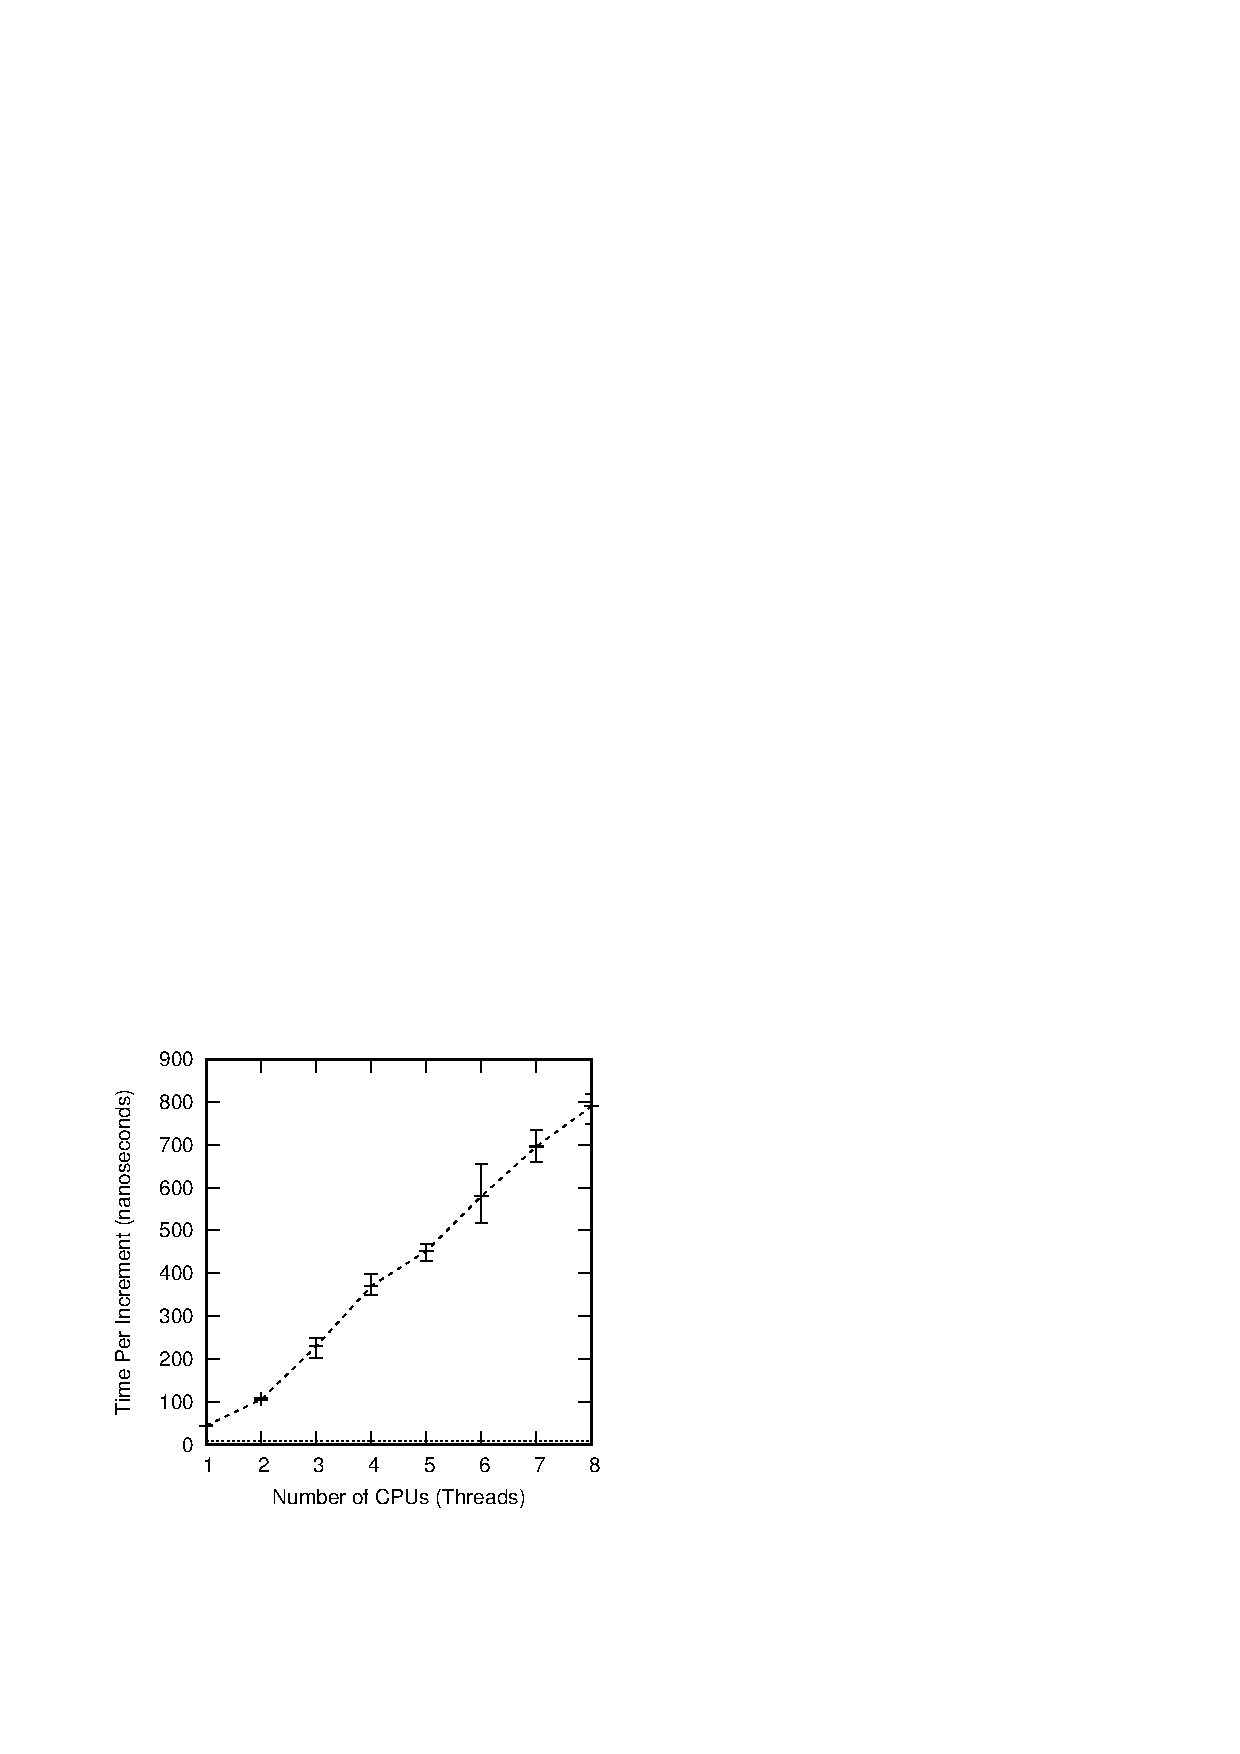
\includegraphics{CodeSamples/count/atomic}}
\caption{Atomic Increment Scalability on Nehalem}
\label{fig:count:Atomic Increment Scalability on Nehalem}
\end{figure}

정확하게 카운트를 하는 직관적 방법은
Listing~\ref{lst:count:Just Count Atomically!} (\path{count_atomic.c})
에 나온 것처럼 어토믹 오퍼레이션을 사용하는 것입니다.
라인~1 은 어토믹 변수를 정의하고, 라인~5 에서 어토믹하게 값을 증가시키고,
라인~10 에서 읽어냅니다.
이건 어토믹하기 때문에, 완벽한 카운트를 유지합니다.
하지만, 느립니다: Intel Core Duo 랩탑에서 이것은 어토믹하지 않은 방법에 비해
싱글쓰레드에서 여섯배, 그리고 두 쓰레드를 사용했을 때엔 \emph{열 배}
느립니다.\footnote{
	흥미롭게도, 어토믹하지 않게 카운터를 증가시키는 두개의 쓰레드는
	어토믹하게 카운터를 증가시키는 두개의 쓰레드보다 더 빨리 그 값을
	증가시킵니다.
	물론, 당신의 목표가 단순히 카운터를 더 빨리 증가시키는 거라면, 그냥
	카운터에 큰 값을 넣으면 되겠습니다.
	그러나, 거대한 성능과 확장성을 위해선 정확성을 주의깊게 완화한
	알고리즘의 역할도 있을 수
	있습니다~\cite{Andrews91textbook,Arcangeli03,DavidUngar2011unsync}.}
\iffalse

The straightforward way to count accurately is to use atomic operations,
as shown in
Listing~\ref{lst:count:Just Count Atomically!} (\path{count_atomic.c}).
Line~1 defines an atomic variable, line~5 atomically increments it, and
line~10 reads it out.
Because this is atomic, it keeps perfect count.
However, it is slower: on a Intel Core Duo laptop, it is about
six times slower than non-atomic increment
when a single thread is incrementing, and more than \emph{ten times}
slower if two threads are incrementing.\footnote{
	Interestingly enough, a pair of threads non-atomically incrementing
	a counter will cause the counter to increase more quickly than
	a pair of threads atomically incrementing the counter.
	Of course, if your only goal is to make the counter increase
	quickly, an easier approach is to simply assign a large value
	to the counter.
	Nevertheless, there is likely to be a role for algorithms that
	use carefully relaxed notions of correctness in order to gain
	greater performance and
	scalability~\cite{Andrews91textbook,Arcangeli03,DavidUngar2011unsync}.}
\fi

Chapter~\ref{chp:Hardware and its Habits} 에서 이야기했던 걸 떠올려 보면
성능이 느린 것도,
Figure~\ref{fig:count:Atomic Increment Scalability on Nehalem} 에서 보여지듯
어토믹 증가 연산의 성능이 CPU 와 쓰레드의 숫자가 증가할수록 느려지는 것도
그다지 놀라운 일은 아닙니다.
이 그림에서, x~축에 붙어있는 수평의 점선은 완벽하게 확장하는 알고리즘에
의해서만 얻어질 수 있는 이상적인 성능입니다: 그런 알고리즘이라면, 카운트 증가는
싱글쓰레드에서와 동일한 오버헤드만을 일으킬 것입니다.
하나의 전역 변수에 대한 어토믹 증가 연산은 분명하게 이상적이지 않으며, CPU 를
추가할수록 성능이 나빠집니다.
\iffalse

This poor performance should not be a surprise, given the discussion in
Chapter~\ref{chp:Hardware and its Habits},
nor should it be a surprise that the performance of atomic increment
gets slower as the number of CPUs and threads increase, as shown in
Figure~\ref{fig:count:Atomic Increment Scalability on Nehalem}.
In this figure, the horizontal dashed line resting on the x~axis
is the ideal performance that would be achieved
by a perfectly scalable algorithm: with such an algorithm, a given
increment would incur the same overhead that it would in a single-threaded
program.
Atomic increment of a single global variable is clearly
decidedly non-ideal, and gets worse as you add CPUs.
\fi

\QuickQuiz{}
	왜 x~축의 점선은 $x=1$ 에서 대각선의 선과 만나지 않죠?
	\iffalse

	Why doesn't the dashed line on the x~axis meet the 
	diagonal line at $x=1$?
	\fi
\QuickQuizAnswer{
	어토믹 오퍼레이션의 오버헤드 때문입니다.
	x~축의 점선은 \emph{어토믹하지 않은} 증가 연산의 싱글쓰레드 수행에서의
	오버헤드를 나타냅니다.
	\emph{이상적인} 알고리즘은 선형적으로 확장될 뿐만 아니라, 싱글 쓰레드
	코드에 비해서도 성능 하락이 없어야 할 것입니다.

	이런 수준의 이상론은 좀 지나쳐 보일 수 있습니다, 다만 리누스 토발즈에게
	충분하다면, 당신에게도 충분할 겁니다.
	\iffalse

	Because of the overhead of the atomic operation.
	The dashed line on the x~axis represents the overhead of
	a single \emph{non-atomic} increment.
	After all, an \emph{ideal} algorithm would not only scale
	linearly, it would also incur no performance penalty compared
	to single-threaded code.

	This level of idealism may seem severe, but if it is good
	enough for Linus Torvalds, it is good enough for you.
	\fi
} \QuickQuizEnd

\QuickQuiz{}
	하지만 어토믹 증가 연산은 여전히 꽤 빠릅니다.
	그리고 빡빡한 루프에서 하나의 변수를 증가시키는 건 제겐 꽤 비현실적인
	것 같아 보이구요, 무엇보다, 프로그램의 실행은 실제로 일을 하는데
	쓰여야지, 자기가 한 일을 세는데 쓰여야 하는게 아니라구요!
	왜 제가 이걸 빠르게 하는걸 고민해야 하나요?
	\iffalse

	But atomic increment is still pretty fast.
	And incrementing a single variable in a tight loop sounds
	pretty unrealistic to me, after all, most of the program's
	execution should be devoted to actually doing work, not accounting
	for the work it has done!
	Why should I care about making this go faster?
	\fi
\QuickQuizAnswer{
	많은 경우에 어토믹 증가 연산은 분명히 당신에겐 충분히 빠를 겁니다.
	그런 경우에 당신은 당연히 어토믹 증가 연산을 사용해야죠.
	그렇지만, 더 나은 카운팅 알고리즘이 필요한 실제 상황도 상당히 많이
	존재합니다.
	그런 상황의 예는 고도로 최적화된 네트워킹 스택에서의 패킷과 용량
	카운팅으로, 이런 예에서는, 특히나 커다란 멀티프로세서에서는 대부분의
	실행시간을 이런류의 카운팅 작업에 보내게 됩니다.

	게다가, 이 챕터의 시작에서 이야기했듯, 카운팅은 공유 메모리 병렬
	프로그램에서 마주칠 수 있는 문제들을 보여줍니다.
	\iffalse

	In many cases, atomic increment will in fact be fast enough
	for you.
	In those cases, you should by all means use atomic increment.
	That said, there are many real-world situations where
	more elaborate counting algorithms are required.
	The canonical example of such a situation is counting packets
	and bytes in highly optimized networking stacks, where it is
	all too easy to find much of the execution time going into
	these sorts of accounting tasks, especially on large
	multiprocessors.

	In addition, as noted at the beginning of this chapter,
	counting provides an excellent view of the
	issues encountered in shared-memory parallel programs.
	\fi
} \QuickQuizEnd

\begin{figure}[tb]
\centering
\resizebox{3in}{!}{\includegraphics{count/GlobalInc}}
\caption{Data Flow For Global Atomic Increment}
\label{fig:count:Data Flow For Global Atomic Increment}
\end{figure}

\begin{figure}[tb]
\centering
\resizebox{3.2in}{!}{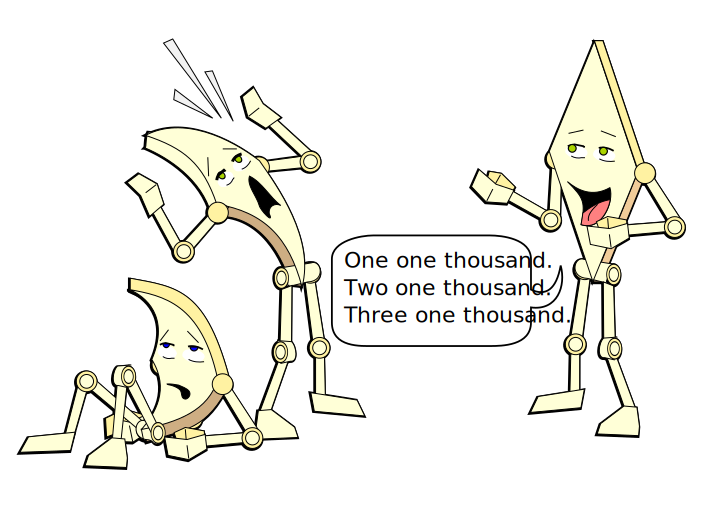
\includegraphics{cartoons/r-2014-One-one-thousand}}
\caption{Waiting to Count}
\ContributedBy{Figure}{fig:count:Waiting to Count}{Melissa Broussard}
\end{figure}

전역 어토믹 증가에 대한 다른 관점을 위해,
Figure~\ref{fig:count:Data Flow For Global Atomic Increment} 를 보세요.
각 CPU 가 주어진 전역 변수를 증가시킬 기회를 얻기 위해서, 해당 변수를 가지고
있는 캐시 라인은 빨간 화살표로 표시된 것처럼 모든 CPU 사이를 순환해야 합니다.
이런 순환은 상당한 시간을 요할 것이고, 이는
Figure~\ref{fig:count:Waiting to Count} 와 같은 상황을 초래해서
Figure~\ref{fig:count:Atomic Increment Scalability on Nehalem} 에서 보여진 낮은
성능을 야기할 것입니다.

다음 섹션들에서는 이런 순환에서 발생하는 지연들을 없앤 고성능 카운팅에 대해
알아봅니다.
\iffalse

For another perspective on global atomic increment, consider
Figure~\ref{fig:count:Data Flow For Global Atomic Increment}.
In order for each CPU to get a chance to increment a given
global variable, the cache line containing that variable must
circulate among all the CPUs, as shown by the red arrows.
Such circulation will take significant time, resulting in
the poor performance seen in
Figure~\ref{fig:count:Atomic Increment Scalability on Nehalem},
which might be thought of as shown in
Figure~\ref{fig:count:Waiting to Count}.

The following sections discuss high-performance counting, which
avoids the delays inherent in such circulation.
\fi

\QuickQuiz{}
	그런데 왜 CPU 설계자들은 단순히 데이터에의 증가 연산을 추가함으로써
	데이터를 담고 있는 캐시 라인의 순환이 증가하는걸 막지 못한 거죠?
	\iffalse

	But why can't CPU designers simply ship the addition operation to the
	data, avoiding the need to circulate the cache line containing
	the global variable being incremented?
	\fi
\QuickQuizAnswer{
	어떤 경우에는 그런 방법도 가능하겠죠.
	하지만, 그러려면 좀 복잡합니다:
	\iffalse

	It might well be possible to do this in some cases.
	However, there are a few complications:
	\fi
	\begin{enumerate}
	\item	만약 어떤 변수의 값이 필요하다면, 값을 필요로 하는 쓰레드는
		해당 오퍼레이션이 그 데이터로 향할 때까지 기다리고, 그러고나선
		돌아오기까지 기다려야 합니다.
	\item	그 어토믹 증가 오퍼레이션이 이전의, 그리고 이후의
		오퍼레이션들과 순서를 맞춰야 한다면, 해당 쓰레드는 오퍼레이션이
		데이터까지 가고, 돌아올 준비가 완료될 때까지 기다려야 합니다.
	\item	오퍼레이션들을 CPU들 사이에서 보내게 되면 시스템 접속부를
		지나야 하고, 이는 더 많은 다이 공간과 전력을 소모하게 될겁니다.
	\iffalse

	\item	If the value of the variable is required, then the
		thread will be forced to wait for the operation
		to be shipped to the data, and then for the result
		to be shipped back.
	\item	If the atomic increment must be ordered with respect
		to prior and/or subsequent operations, then the thread
		will be forced to wait for the operation to be shipped
		to the data, and for an indication that the operation
		completed to be shipped back.
	\item	Shipping operations among CPUs will likely require
		more lines in the system interconnect, which will consume
		more die area and more electrical power.
	\fi
	\end{enumerate}
	하지만 앞의 두가지 조건이 없다면?
	그럼 여러분은 Section~\ref{sec:count:Statistical Counters} 에서
	논의되는, 실제 상품화된 하드웨어에서 이상적 상황에 근접하는 성능을
	보이는 알고리즘을 잘 고려해 봐야 할 겁니다.
	\iffalse

	But what if neither of the first two conditions holds?
	Then you should think carefully about the algorithms discussed
	in Section~\ref{sec:count:Statistical Counters}, which achieve
	near-ideal performance on commodity hardware.
	\fi

\begin{figure}[tb]
\centering
\resizebox{3in}{!}{\includegraphics{count/GlobalTreeInc}}
\caption{Data Flow For Global Combining-Tree Atomic Increment}
\label{fig:count:Data Flow For Global Combining-Tree Atomic Increment}
\end{figure}

	앞의 두개 조건이 모두, 또는 하나라도 걸려 있다면, 개선된 하드웨어에
	\emph{약간}의 희망이 있습니다.
	컴바이닝 트리(combining tree) 를 하드웨어에서 구현해서, 여러 CPU 에서의
	증가 요청이 하드웨어에 의해 결합되어 하나의 더하기 연산으로 변환되는
	방법을 생각해 볼 수 있을 것입니다.
	해당 하드웨어는 또한 요청들에 순서를 잡아줄 수도 있으므로, 각 CPU 에게
	각자의 어토믹 증가에 의한 값의 반환도 가능할 겁니다.
	Figure~\ref{fig:count:Data Flow For Global Combining-Tree Atomic Increment}
	에서 보여지듯, 이는 인스트럭션의 대기시간을 $O(log N)$ 로 만들어
	줍니다. 여기서 $N$ 은 CPU 의 갯수입니다.
	그리고 이런 하드웨어 최적화를 포함하는 CPU 는 2011년부터 나오기
	시작했습니다.

	Figure~\ref{fig:count:Data Flow For Global Atomic Increment} 에 보여진
	현재 하드웨어의 $O(N)$ 성능에 비하면 엄청난 향상이고, 3차원 제조 공정이
	현실화되면 하드웨어 응답시간은 더욱 낮아질 수 있을 겁니다.
	물론, 일부 중요한 특수 케이스에서는 소프트웨어가 \emph{훨씬} 나은 일을
	할 수 있을 것입니다.
	\iffalse

	If either or both of the first two conditions hold, there is
	\emph{some} hope for improved hardware.
	One could imagine the hardware implementing a combining tree,
	so that the increment requests from multiple CPUs are combined
	by the hardware into a single addition when the combined request
	reaches the hardware.
	The hardware could also apply an order to the requests, thus
	returning to each CPU the return value corresponding to its
	particular atomic increment.
	This results in instruction latency that varies as $\O{\log N}$,
	where $N$ is the number of CPUs, as shown in
	Figure~\ref{fig:count:Data Flow For Global Combining-Tree Atomic Increment}.
	And CPUs with this sort of hardware optimization are starting to
	appear as of 2011.

	This is a great improvement over the $\O{N}$ performance
	of current hardware shown in
	Figure~\ref{fig:count:Data Flow For Global Atomic Increment},
	and it is possible that hardware latencies might decrease
	further if innovations such as three-dimensional fabrication prove
	practical.
	Nevertheless, we will see that in some important special cases,
	software can do \emph{much} better.
	\fi
} \QuickQuizEnd

\section{Statistical Counters}
\label{sec:count:Statistical Counters}

이 섹션은 카운트는 매우 자주 업데이트 되지만 매우 가끔씩만 그 값이 읽혀지는,
통계적 카운터의 흔한 특수 케이스들을 다룹니다.
이것들은 \QuickQuizRef{\QcountQstatcnt} 에서 이야기한 네트워크 패킷 카운팅
문제를 푸는데 사용되곤 할 겁니다.
\iffalse

This section covers the common special case of statistical counters, where
the count is updated extremely frequently and the value is read out
rarely, if ever.
These will be used to solve the network-packet counting problem
posed in \QuickQuizRef{\QcountQstatcnt}.
\fi

\subsection{Design}

통계적 카운팅은 보통 쓰레드별로 (또는, 커널에서라면 CPU별로) 카운터를 제공해서
각 쓰레드가 자신의 카운터를 업데이트 하도록 합니다.
이 카운터들의 전체 통합 값은 더하기의 상호성과 결합성에 기반해, 단순히 모든
쓰레드의 카운터의 값을 더하는 것으로 구해질 수 있습니다.
이건 Section~\ref{sec:SMPdesign:Data Ownership} 에서 소개될 데이터 소유권
패턴의 한 예입니다.
\iffalse

Statistical counting is typically handled by providing a counter per
thread (or CPU, when running in the kernel), so that each thread
updates its own counter.
The aggregate value of the counters is read out by simply summing up
all of the threads' counters,
relying on the commutative and associative properties of addition.
This is an example of the Data Ownership pattern that will be introduced in
Section~\ref{sec:SMPdesign:Data Ownership}.
\fi

\QuickQuiz{}
	하지만 C 의 ``정수들'' 의 제한된 크기가 일을 복잡하게 만들지는 않나요?
	\iffalse

	But doesn't the fact that C's ``integers'' are limited in size
	complicate things?
	\fi
\QuickQuizAnswer{
	아닙니다, 모듈로 더하기도 역시 상호성과 결합성을 가지니까요.
	부호 없는 정수형을 사용한다면 말입니다.
	오버플로우가 났을 때 넘쳐난 값을 감추는 것 외에 별다른 일을 하는
	기계들은 요즘 거의 없지만, C 표준에 의하면 부호를 갖는 정수형의
	오버플로우는 예상외 동작을 유발할 수 있으므로, 요즘 기계들은 대부분
	안전하다는 사실은 무시하십시오.
	불행히도, 컴파일러들은 종종 부호 있는 정수형들은 오버플로우 나지 않을
	것이라는 가정 하에 최적화를 하기 때문에, 당신의 코드가 부호 있는
	정수형을 오버플로우 나게 한다면, 2의 보수를 사용하는 하드웨어를
	사용하고 있다 해도 문제에 직면할 수 있습니다.

	그렇다곤 해도, 32-비트 쓰레드별 카운터에서 (대략) 64-비트 합을
	모으는데에도 추가적인 복잡한 일이 숨어있습니다.
	이걸 처리하는 것은 독자 여러분의 연습문제로 남겨두겠습니다만, 이 챕터의
	뒤에 소개될 기법들이 큰 도움이 될 수도 있습니다.
	\iffalse

	No, because modulo addition is still commutative and associative.
	At least as long as you use unsigned integers.
	Recall that in the C standard, overflow of signed integers results
	in undefined behavior, never mind the fact that machines that
	do anything other than wrap on overflow are quite rare these days.
	Unfortunately, compilers frequently carry out optimizations that
	assume that signed integers will not overflow, so if your code
	allows signed integers to overflow, you can run into trouble
	even on twos-complement hardware.

	That said, one potential source of additional complexity arises
	when attempting to gather (say) a 64-bit sum from 32-bit
	per-thread counters.
	Dealing with this added complexity is left as
	an exercise for the reader, for whom some of the techniques
	introduced later in this chapter could be quite helpful.
	\fi
} \QuickQuizEnd

\subsection{Array-Based Implementation}
\label{sec:count:Array-Based Implementation}

쓰레드별 변수를 제공하는 방법 중 하나는 쓰레드별로 (false sharing 을 막기 위해
캐시 라인 크기에 맞춰 정렬 되어있고 채워져 있는)원소 하나를 갖는 배열을 만드는
겁니다.
\iffalse

One way to provide per-thread variables is to allocate an array with
one element per
thread (presumably cache aligned and padded to avoid false sharing).
\fi

\QuickQuiz{}
	배열이요???
	하지만 그럼 쓰레드의 갯수가 제한되지 않나요?
	\iffalse

	An array???
	But doesn't that limit the number of threads?
	\fi
\QuickQuizAnswer{
	그럴 수 있고, 이 간단한 구현에서는 그렇습니다.
	하지만 임의의 갯수의 쓰레드를 지원하는 구현을 만드는 건 그렇게 어렵지
	않은데, 예를 들면,
	Section~\ref{sec:count:Per-Thread-Variable-Based Implementation}
	\GCC 의 \co{__thread} 를 사용하는 거죠.
	\iffalse

	It can, and in this toy implementation, it does.
	But it is not that hard to come up with an alternative
	implementation that permits an arbitrary number of threads,
	for example, using \GCC's \co{__thread} facility,
	as shown in
	Section~\ref{sec:count:Per-Thread-Variable-Based Implementation}.
	\fi
} \QuickQuizEnd

\begin{listing}[tbp]
{ \scriptsize
\begin{verbbox}
  1 DEFINE_PER_THREAD(long, counter);
  2 
  3 void inc_count(void)
  4 {
  5   __get_thread_var(counter)++;
  6 }
  7 
  8 long read_count(void)
  9 {
 10   int t;
 11   long sum = 0;
 12 
 13   for_each_thread(t)
 14     sum += per_thread(counter, t);
 15   return sum;
 16 }
\end{verbbox}
}
\centering
\theverbbox
\caption{Array-Based Per-Thread Statistical Counters}
\label{lst:count:Array-Based Per-Thread Statistical Counters}
\end{listing}

그런 배열은
Listing~\ref{lst:count:Array-Based Per-Thread Statistical Counters}
(\path{count_stat.c}) 에 보여진 것처럼 per-thread 기능을 사용할 수도 있습니다.
라인~1 은 \co{long} 타입의 쓰레드별 카운터들을 담는, \co{counter} 라는 이름의
배열을 정의합니다.

라인~3-6 은 이 카운터를 증가시키는 함수로, \co{__get_thread_var()} 함수를
사용해 \co{counter} 배열에서 현재 수행중인 쓰레드의 원소를 얻어옵니다.
이 원소는 연관된 쓰레드에 의해서만 수정되므로, 어토믹하지 않은 방식으로도
충분합니다.

라인~8-16 은 카운터의 전체 값을 얻어오는 함수로, \co{for_each_thread()} 를
이용해 현재 돌고 있는 쓰레드들의 리스트를 순회하면서 \co{per_thread()} 를
이용해 특정 쓰레드의 카운터 값을 얻어옵니다.
하드웨어는 제대로 정렬되어 있는 \co{long} 변수는 어토믹하게 읽고 쓸 수 있기
때문에, 그리고 \GCC\ 는 이 기능을 잘 사용해주기 때문에, 평범한 읽기로 충분하고,
별다른 어토믹 오퍼레이션은 필요치 않습니다.
\iffalse

Such an array can be wrapped into per-thread primitives, as shown in
Listing~\ref{lst:count:Array-Based Per-Thread Statistical Counters}
(\path{count_stat.c}).
Line~1 defines an array containing a set of per-thread counters of
type \co{long} named, creatively enough, \co{counter}.

Lines~3-6 show a function that increments the counters, using the
\co{__get_thread_var()} primitive to locate the currently running
thread's element of the \co{counter} array.
Because this element is modified only by the corresponding thread,
non-atomic increment suffices.

Lines~8-16 show a function that reads out the aggregate value of the counter,
using the \co{for_each_thread()} primitive to iterate over the list of
currently running threads, and using the \co{per_thread()} primitive
to fetch the specified thread's counter.
Because the hardware can fetch and store a properly aligned \co{long}
atomically, and because \GCC\ is kind enough to make use of this capability,
normal loads suffice, and no special atomic instructions are required.
\fi

\QuickQuiz{}
	근데, 그 외에 \GCC\ 가 어떤 짓을 할 수 있죠???
	\iffalse

	What other choice does \GCC\ have, anyway???
	\fi
\QuickQuizAnswer{
	C 표준대로라면, 다른 쓰레드에 의해 동시에 수정되고 있을 수 있는 변수를
	읽어들이는 행동의 효과에 대해선 정의되어 있지 않습니다.
	C 는 어토믹하게 \co{long} 타입 변수를 읽어들일 수가 없는 (예를
	들면) 8-비트 아키텍쳐를 지원해야만 했기에 C 표준은 다른 선택의 여지가
	없었습니다.
	다음 버전의 C 표준에서는 이 현실과의 격차를 해결해 보려 합니다만, 그
	전까지는 \GCC\ 개발자들의 친절함에 의존해야 합니다.

	대신, 하드웨어가 한번의 메모리 참조 명령으로 필요한 값을 읽을 수 있는
	경우라면, \co{READ_ONCE()} 와 \co{WRITE_ONCE()} 에 의해 제공되는
	volatile 접근을 사용해서 컴파일러에 제약을 가할 수 있습니다.\footnote{
		\co{READ_ONCE()} 와 \co{WRITE_ONCE()} 의 간단한 정의가
		Listing~\ref{lst:toolsoftrade:Compiler Barrier Primitive (for
		GCC)}에 보여져 있습니다.}
	\iffalse

	According to the C standard, the effects of fetching a variable
	that might be concurrently modified by some other thread are
	undefined.
	It turns out that the C standard really has no other choice,
	given that C must support (for example) eight-bit architectures
	which are incapable of atomically loading a \co{long}.
	An upcoming version of the C standard aims to fill this gap,
	but until then, we depend on the kindness of the \GCC\ developers.

	Alternatively, use of volatile accesses such as those provided
	by \co{READ_ONCE()} and \co{WRITE_ONCE()} can help constrain
	the compiler,\footnote{
		Simple definitions of \co{READ_ONCE()} and
		\co{WRITE_ONCE()} are shown in
		Listing~\ref{lst:toolsoftrade:Compiler Barrier Primitive (for GCC)}.}
	at least
	in cases where the hardware is capable of accessing the value
	with a single memory-reference instruction.
	\fi
} \QuickQuizEnd

\QuickQuiz{}
	Listing~\ref{lst:count:Array-Based Per-Thread Statistical Counters} 의
	쓰레드별 \co{counter} 변수는 어떻게 초기화 되나요?
	\iffalse

	How does the per-thread \co{counter} variable in
	Listing~\ref{lst:count:Array-Based Per-Thread Statistical Counters}
	get initialized?
	\fi
\QuickQuizAnswer{
	C 표준은 전역 변수의 초기값은 명시적으로 초기화되지 않는 이상 0이라고
	명시합니다.
	따라서 \co{counter} 의 모든 인스턴스의 초기값은 0이 될겁니다.
	그리고, 사용자가 통계적 카운터들의 연속적으로 읽어들이는 값 사이의
	차이에만 관심있는 일반적인 경우에는 초기값은 의미가 없습니다.
	\iffalse

	The C standard specifies that the initial value of
	global variables is zero, unless they are explicitly initialized.
	So the initial value of all the instances of \co{counter}
	will be zero.
	Furthermore, in the common case where the user is interested only
	in differences between consecutive reads
	from statistical counters, the initial value is irrelevant.
	\fi
} \QuickQuizEnd

\QuickQuiz{}
	Listing~\ref{lst:count:Array-Based Per-Thread Statistical Counters}
	의 코드가 어떻게 복수의 카운터를 가능하게 할 수 있죠?
	\iffalse

	How is the code in
	Listing~\ref{lst:count:Array-Based Per-Thread Statistical Counters}
	supposed to permit more than one counter?
	\fi
\QuickQuizAnswer{
	실제로, 이 예제는 한개 이상의 카운터는 지원하지 않습니다.
	이 예제를 수정해서 복수의 카운터를 제공하게 하는건 독자 여러분에게
	과제로 남겨 두겠습니다.
	\iffalse

	Indeed, this toy example does not support more than one counter.
	Modifying it so that it can provide multiple counters is left
	as an exercise to the reader.
	\fi
} \QuickQuizEnd

\begin{figure}[tb]
\centering
\resizebox{3in}{!}{\includegraphics{count/PerThreadInc}}
\caption{Data Flow For Per-Thread Increment}
\label{fig:count:Data Flow For Per-Thread Increment}
\end{figure}

이 방법은 \co{inc_count()} 를 호출하는 업데이터 쓰레드의 수가 늘어나더라도
선형적으로 성능이 확장됩니다.
Figure~\ref{fig:count:Data Flow For Per-Thread Increment} 의 각 CPU 위의 초록색
화살표로 보여지듯, 각 CPU 는 시스템 사이를 통과하는 비싼 비용의 통신 없이
자신의 쓰레드의 변수를 빠르게 증가시킬 수 있기 때문입니다.
이와 같이, 이 섹션은 이 챕터의 시작에서 소개된 네트워크 패킷 카운팅 문제를
해결합니다.
\iffalse

This approach scales linearly with increasing number of updater threads
invoking \co{inc_count()}.
As is shown by the green arrows on each CPU in
Figure~\ref{fig:count:Data Flow For Per-Thread Increment},
the reason for this is that each CPU can make rapid progress incrementing
its thread's variable, without any expensive cross-system communication.
As such, this section solves the network-packet counting problem presented
at the beginning of this chapter.
\fi

\QuickQuiz{}
	읽기 오퍼레이션은 쓰레드별 값을 모두 더하는 시간을 가져야 할 것이고,
	그동안에도 카운터는 값이 변할 수 있어요.
	이는,
	Listing~\ref{lst:count:Array-Based Per-Thread Statistical Counters}
	의  \co{read_count()} 는 정확하지 않다는 것을 의미합니다.
	이 카운터는 단위시간당 $r$ 만큼 값이 증가되고 \co{read_count()} 는
	$\Delta$ 단위시간을 소모한다고 해봅시다.
	반환되는 값의 예상 오류값은 얼마입니까?
	\iffalse

	The read operation takes time to sum up the per-thread values,
	and during that time, the counter could well be changing.
	This means that the value returned by
	\co{read_count()} in
	Listing~\ref{lst:count:Array-Based Per-Thread Statistical Counters}
	will not necessarily be exact.
	Assume that the counter is being incremented at rate
	$r$ counts per unit time, and that \co{read_count()}'s
	execution consumes $\Delta$ units of time.
	What is the expected error in the return value?
	\fi
\QuickQuizAnswer{
	최악의 경우에 대한 분석부터 해보고, 좀 나은 경우들을 보죠.

	최악의 경우는, 읽기 오퍼레이션이 실제 동작은 금방 끝냈지만 리턴하기
	전에 $\Delta$ 단위시간동안 대기를 하는 경우로, 이 경우의 오류값은
	간단히 $r \Delta$ 입니다.
	\iffalse

	Let's do worst-case analysis first, followed by a less
	conservative analysis.

	In the worst case, the read operation completes immediately,
	but is then delayed for $\Delta$ time units before returning,
	in which case the worst-case error is simply $r \Delta$.
	\fi

	이 최악의 경우 동작은 별로 현실성이 없으니 각 $N$ 카운터들에 대한 각
	읽기 동작이 시간 간격 $\Delta$ 안에 동일한 간격으로 일어나는 경우를
	생각해보죠.
	$N$ 회의 읽기 사이에 $\frac{\Delta}{N+1}$ 길이의 $N+1$ 개 간격이 존재할
	겁니다.
	마지막 쓰레드의 카운터에서의 읽기 이후로의 지연으로 발생하는 에러치는
	$\frac{r \Delta}{N \left( N + 1 \right)}$ 이므로, 두번째에서 마지막
	쓰레드 사이의 카운터는
	$\frac{2 r \Delta}{N \left( N + 1 \right)}$,
	세번째에서 마지막 사이는
	$\frac{3 r \Delta}{N \left( N + 1 \right)}$,
	그리고 그렇게 계속 진행됩니다.
	전체 오류값은 각 쓰레드의 카운터에서의 읽기로 발생한 에러의 총 합으로
	주어지는데, 다음과 같습니다:

	\begin{equation}
		\frac{r \Delta}{N \left( N + 1 \right)}
			\sum_{i = 1}^N i
	\end{equation}
	\iffalse

	This worst-case behavior is rather unlikely, so let us instead
	consider the case where the reads from each of the $N$
	counters is spaced equally over the time period $\Delta$.
	There will be $N+1$ intervals of duration $\frac{\Delta}{N+1}$
	between the $N$ reads.
	The error due to the delay after the read from the last thread's
	counter will be given by $\frac{r \Delta}{N \left( N + 1 \right)}$,
	the second-to-last thread's counter by
	$\frac{2 r \Delta}{N \left( N + 1 \right)}$,
	the third-to-last by
	$\frac{3 r \Delta}{N \left( N + 1 \right)}$,
	and so on.
	The total error is given by the sum of the errors due to the
	reads from each thread's counter, which is:

	\begin{equation}
		\frac{r \Delta}{N \left( N + 1 \right)}
			\sum_{i = 1}^N i
	\end{equation}
	\fi

	합 부분은 다음과 같이 표현 가능하구요:

	\begin{equation}
		\frac{r \Delta}{N \left( N + 1 \right)}
			\frac{N \left( N + 1 \right)}{2}
	\end{equation}

	불필요한 부분을 제거하면 다음과 같이 직관적인 결과가 나옵니다:

	\begin{equation}
		\frac{r \Delta}{2}
	\label{eq:count:CounterErrorAverage}
	\end{equation}
	\iffalse

	Expressing the summation in closed form yields:

	\begin{equation}
		\frac{r \Delta}{N \left( N + 1 \right)}
			\frac{N \left( N + 1 \right)}{2}
	\end{equation}

	Cancelling yields the intuitively expected result:

	\begin{equation}
		\frac{r \Delta}{2}
	\label{eq:count:CounterErrorAverage}
	\end{equation}
	\fi

	읽기 오퍼레이션 호출자가 해당 오퍼레이션으로 리턴받은 수를 가지고 어떤
	일을 하는 코드를 수행하는 중에도 오류는 쌓여감을 기억해둘 필요가
	있습니다.
	예를 들어, 읽기 오퍼레이션 호출자가 리턴받은 값을 가지고 어떤 계산을
	하는데 $t$ 시간을 사용한다면, 최악의 경우 오류치는 $r \left(\Delta +
	t\right)$ 로 늘어날 겁니다.

	예상 오류치도 비슷하게 늘어나겠죠:
	\iffalse

	It is important to remember that error continues accumulating
	as the caller executes code making use of the count returned
	by the read operation.
	For example, if the caller spends time $t$ executing some
	computation based on the result of the returned count, the
	worst-case error will have increased to $r \left(\Delta + t\right)$.

	The expected error will have similarly increased to:
	\fi

	\begin{equation}
		r \left( \frac{\Delta}{2} + t \right)
	\end{equation}

	물론, 읽기 중에 카운터가 계속 증가하는건 용납될 수 없는 경우도
	있겠습니다.
	Section~\ref{sec:count:Applying Specialized Parallel Counters}
	에서는 이런 상황을 해결하는 방법을 알아봅니다.

	이렇게, 우리는 감소는 없고 증가만 이루어지는 카운터를 알아보았습니다.
	만약 카운터 값이 단위시간당 $r$ 만큼 감소되든 증가되든 바뀐다면,
	오류값은 줄어들 거라고 예상할 수 있을 겁니다.
	하지만, 카운터가 어느 쪽으로든 움직일 수 \emph{있을지 몰라도} 최악의
	경우는 해당 읽기 오퍼레이션이 금방 끝났지만 $\Delta$ 단위 시간동안
	기다려야 하는데, 그 시간 동안 카운터의 값은 같은 방향으로만 이동하는
	경우이므로 여전히 $r \Delta$ 오류값을 내므로 차이가 없습니다.
	\iffalse

	Of course, it is sometimes unacceptable for the counter to
	continue incrementing during the read operation.
	Section~\ref{sec:count:Applying Specialized Parallel Counters}
	discusses a way to handle this situation.

	Thus far, we have been considering a counter that is only
	increased, never decreased.
	If the counter value is being changed by $r$ counts per unit
	time, but in either direction, we should expect the error
	to reduce.
	However, the worst case is unchanged because although the
	counter \emph{could} move in either direction, the worst
	case is when the read operation completes immediately,
	but then is delayed for $\Delta$ time units, during which
	time all the changes in the counter's value move it in
	the same direction, again giving us an absolute error
	of $r \Delta$.
	\fi

	평균 에러치를 계산하는데는 값의 증감 패턴에 대한 다양한 가정을 바탕으로
	하는 여러가지 방법이 있습니다.
	일단은 간단하게, 오퍼레이션들 중 $f$ 만큼이 감소 오퍼레이션이고,
	관심있는 오류값은 카운터의 장시간 추세선에서의 굴곡이라고 가정해
	봅시다.
	이 가정 하에서는 $f$ 가 0.5 이하라면, 각 감소는 증가에 의해 무효화
	되고, 따라서 $2f$ 오퍼레이션은 서로를 무효화 시키고, $1-2f$ 의
	오퍼레이션들은 무효화 되지 않은 증가가 됩니다.
	반면, $f$ 가 0.5 보다 크다면, $1-f$ 의 감소는 증가에 의해 무효화 되고,
	카운터는 음의 방향으로 $-1+2\left(1-f\right)$ 만큼 이동하는데, 이는
	$1-2f$ 로 정리되고, 따라서 카운터는 평균적으로 오퍼레이션당 $1-2f$
	만큼씩 어느 경우든 이동하게 됩니다.
	따라서, 긴 시점에서의 카운터의 변화는 $\left( 1-2f \right) r$ 로
	주어집니다.
	이걸 Equation~\ref{eq:count:CounterErrorAverage} 에 대입하면:
	\iffalse

	There are a number of ways to compute the average error,
	based on a variety of assumptions about the patterns of
	increments and decrements.
	For simplicity, let's assume that the $f$ fraction of
	the operations are decrements, and that the error of interest
	is the deviation from the counter's long-term trend line.
	Under this assumption, if $f$ is less than or equal to 0.5,
	each decrement will be cancelled by an increment, so that
	$2f$ of the operations will cancel each other, leaving
	$1-2f$ of the operations being uncancelled increments.
	On the other hand, if $f$ is greater than 0.5, $1-f$ of
	the decrements are cancelled by increments, so that the
	counter moves in the negative direction by $-1+2\left(1-f\right)$,
	which simplifies to $1-2f$, so that the counter moves an average
	of $1-2f$ per operation in either case.
	Therefore, that the long-term
	movement of the counter is given by $\left( 1-2f \right) r$.
	Plugging this into
	Equation~\ref{eq:count:CounterErrorAverage} yields:
	\fi

	\begin{equation}
		\frac{\left( 1 - 2 f \right) r \Delta}{2}
	\end{equation}

	그렇지만, 대부분의 통계적 카운터 사용에서 \co{read_count()} 에 의해
	리턴되는 값의 오류치는 별 의미가 없습니다.
	\co{read_count()} 가 수행하는데 필요한 시간은 일반적으로
	\co{read_count()} 호출 사이의 시간에 비하면 극단적으로 작기 때문입니다.
	\iffalse

	All that aside, in most uses of statistical counters, the
	error in the value returned by \co{read_count()} is
	irrelevant.
	This irrelevance is due to the fact that the time required
	for \co{read_count()} to execute is normally extremely
	small compared to the time interval between successive
	calls to \co{read_count()}.
	\fi
} \QuickQuizEnd

하지만, 이 업데이트 쪽 확장성은 쓰레드의 수가 늘어날 경우 읽기 쪽에 큰 부담으로
다가옵니다.
다음 섹션에서는 업데이트 쪽 확장성을 유지하면서 읽기 쪽 부담을 줄이는 방법을
알아봅니다.
\iffalse

However, this excellent update-side scalability comes at great read-side
expense for large numbers of threads.
The next section shows one way to reduce read-side expense while
still retaining the update-side scalability.
\fi

\subsection{Eventually Consistent Implementation}
\label{sec:count:Eventually Consistent Implementation}

읽기 쪽 성능을 크게 개선하면서 업데이트 쪽 확장성도 지키는 한가지 방법은
일관성에 대한 요구사항을 약화시키는 것입니다.
앞 섹션의 카운팅 알고리즘은 이상적인 카운터가 \co{read_count()} 실행 직전에
내놓을 값과 실행 직후에 내놓을 값 사이의 값을 내놓는 것을 보장했습니다.
\emph{최종적 일관성(Eventual consistency}~\cite{WernerVogels:2009:EventuallyConsistent}
는 더 완화된 보장사항을 제공합니다: \co{inc_count()} 호출이 없을 때라는 조건
하에, \co{read_count()} 는 최종적으로는 정확한 값을 리턴할 것입니다.
\iffalse

One way to retain update-side scalability while greatly improving
read-side performance is to weaken consistency requirements.
The counting algorithm in the previous section is guaranteed to
return a value between the value that an ideal counter would have
taken on near the beginning of \co{read_count()}'s execution and
that near the end of \co{read_count()}'s execution.
\emph{Eventual consistency}~\cite{WernerVogels:2009:EventuallyConsistent}
provides a weaker
guarantee: in absence of calls to \co{inc_count()}, calls to
\co{read_count()} will eventually return an accurate count.
\fi

우리는 글로벌 카운터를 사용해 최종적 일관성을 제공할 것입니다.
하지만, 업데이트 쓰레드는 쓰레드별 카운터만을 사용합니다.
이 쓰레드별 카운터를 글로벌 카운터로 이동시키는 별도의 쓰레드가 제공됩니다.
읽기 쓰레드는 단순히 글로벌 카운터의 값을 읽습니다.
업데이트 쓰레드가 수행 중이라면, 읽기 쓰레드가 읽어낸 값은 과거의 값일
것입니다만, 일단 업데이트가 중단되면 글로벌 카운터는 최종적으로 진짜 값을 가질
겁니다---따라서 이 방법은 최종적 일관성에 부합합니다.
\iffalse

We exploit eventual consistency by maintaining a global counter.
However, updaters only manipulate their per-thread counters.
A separate thread is provided to transfer counts from the per-thread
counters to the global counter.
Readers simply access the value of the global counter.
If updaters are active, the value used by the readers will be out of
date, however, once updates cease, the global counter will eventually
converge on the true value---hence this approach qualifies as
eventually consistent.
\fi

\begin{listing}[tbp]
{ \scriptsize
\begin{verbbox}
 1 DEFINE_PER_THREAD(unsigned long, counter);
 2 unsigned long global_count;
 3 int stopflag;
 4
 5 void inc_count(void)
 6 {
 7   WRITE_ONCE(__get_thread_var(counter),
 8              READ_ONCE(__get_thread_var(counter)) + 1);
 9 }
10
11 unsigned long read_count(void)
12 {
13   return READ_ONCE(global_count);
14 }
15
16 void *eventual(void *arg)
17 {
18   int t;
19   unsigned long sum;
20
21   while (READ_ONCE(stopflag) < 3) {
22     sum = 0;
23     for_each_thread(t)
24       sum += READ_ONCE(per_thread(counter, t));
25     WRITE_ONCE(global_count, sum);
26     poll(NULL, 0, 1);
27     if (READ_ONCE(stopflag)) {
28       smp_mb();
29       WRITE_ONCE(stopflag, READ_ONCE(stopflag) + 1);
30     }
31   }
32   return NULL;
33 }
34
35 void count_init(void)
36 {
37   thread_id_t tid;
38
39   if (pthread_create(&tid, NULL, eventual, NULL) != 0) {
40     perror("count_init:pthread_create");
41     exit(-1);
42   }
43 }
44
45 void count_cleanup(void)
46 {
47   WRITE_ONCE(stopflag, 1);
48   while (READ_ONCE(stopflag) < 3)
49     poll(NULL, 0, 1);
50   smp_mb();
51 }
\end{verbbox}
}
\centering
\theverbbox
\caption{Array-Based Per-Thread Eventually Consistent Counters}
\label{lst:count:Array-Based Per-Thread Eventually Consistent Counters}
\end{listing}

Listing~\ref{lst:count:Array-Based Per-Thread Eventually Consistent Counters}
(\path{count_stat_eventual.c}) 에 그 구현이 있습니다.
라인~1-2 는 카운터의 값을 갖는 쓰레드별 변수와 글로벌 변수를 보여주며, 세번째
라인은 프로그램을 정확한 카운터 값과 함께 종료하고자 할 경우를 위해 종료 조건을
알리는 \co{stopflag} 를 보입니다.
라인~5-9 의 \co{inc_count()} 함수는
Listing~\ref{lst:count:Array-Based Per-Thread Statistical Counters} 의 것과
비슷합니다.
라인~11-14 의 \co{read_count()} 함수는 단순히 \co{global_count} 변수의 값을
리턴합니다.
\iffalse

The implementation is shown in
Listing~\ref{lst:count:Array-Based Per-Thread Eventually Consistent Counters}
(\path{count_stat_eventual.c}).
Lines~1-2 show the per-thread variable and the global variable that
track the counter's value, and line three shows \co{stopflag}
which is used to coordinate termination (for the case where we want
to terminate the program with an accurate counter value).
The \co{inc_count()} function shown on lines~5-9 is similar to its
counterpart in
Listing~\ref{lst:count:Array-Based Per-Thread Statistical Counters}.
The \co{read_count()} function shown on lines~11-14 simply returns the
value of the \co{global_count} variable.
\fi

하지만, 라인~35-43 의 \co{count_init()} 함수는 라인~16-33 의 \co{eventual()}
쓰레드를 생성하는데, 이 쓰레드는 모든 쓰레드를 순회하며 쓰레드별 로컬
\co{counter} 를 더해서 \co{global_count} 변수에 저장하는 일을 반복합니다.
\co{eventual()} 쓰레드는 일의 반복 사이에 임의로 선택된 1 밀리세컨드 동안
기다립니다.
라인~45-51 의 \co{count_cleanup()} 함수는 프로그램 종료를 관장합니다.

이 방법은 여전히 선형적인 카운터 업데이트 성능을 유지하면서 극단적으로 빠른
카운터 읽기 속도를 보입니다.
하지만, 이 훌륭한 읽기 성능과 업데이트 성능 확장성은 \co{eventual()} 이라는
추가된 쓰레드의 수행이라는 비용을 가집니다.
\iffalse

However, the \co{count_init()} function on lines~35-43
creates the \co{eventual()} thread shown on lines~16-33, which
cycles through all the threads,
summing the per-thread local \co{counter} and storing the
sum to the \co{global_count} variable.
The \co{eventual()} thread waits an arbitrarily chosen one millisecond
between passes.
The \co{count_cleanup()} function on lines~45-51 coordinates termination.

This approach gives extremely fast counter read-out while still
supporting linear counter-update performance.
However, this excellent read-side performance and update-side scalability
comes at the cost of the additional thread running \co{eventual()}.
\fi

\QuickQuiz{}
	Listing~\ref{lst:count:Array-Based Per-Thread Eventually Consistent Counters}
	의 \co{inc_count()} 는 왜 어토믹 명령을 사용하지 않죠?
	쓰레드별 카운터를 여러 쓰레드에서 접근하고 있잖아요!
	\iffalse

	Why doesn't \co{inc_count()} in
	Listing~\ref{lst:count:Array-Based Per-Thread Eventually Consistent Counters}
	need to use atomic instructions?
	After all, we now have multiple threads accessing the per-thread
	counters!
	\fi
\QuickQuizAnswer{
	두 쓰레드 중 하나는 읽기만 하고 있고, 변수는 정렬되어 있으며 기계가
	지원하는 워드 크기이기에, 어토믹하지 않은 명령들만으로도
	충분합니다.
	다만, 카운터 업데이트가 \co{eventual()} 에게 보여지지 않게 할 수도 있는
	컴파일러 최적화를 막기 위해 \co{READ_ONCE()} 매크로가
	사용되었습니다.\footnote{
		\co{READ_ONCE()} 의 간단한 정의가
		Listing~\ref{lst:toolsoftrade:Compiler Barrier Primitive (for GCC)}
		에 표시되어 있습니다.}
	\iffalse

	Because one of the two threads only reads, and because the
	variable is aligned and machine-sized, non-atomic instructions
	suffice.
	That said, the \co{READ_ONCE()} macro is used to prevent
	compiler optimizations that might otherwise prevent the
	counter updates from becoming visible to
	% TODO: Apply
	\co{eventual()}.\footnote{
		A simple definition of \co{READ_ONCE()} is shown in
		Listing~\ref{lst:toolsoftrade:Compiler Barrier Primitive (for GCC)}.}
	\fi

	이 알고리즘의 예전 버전은 실제로 어토믹 명령을 사용했었습니다만,
	감사하게도 Ersoy Bayramoglu 가 그것들이 필요 없다는 것을 지적해
	줬습니다.
	그렇다곤 하나, 쓰레드별 \co{counter} 변수가 \co{global_counter} 보다
	작았다면 어토믹 명령이 필요했을 겁니다.
	하지만, 32-bit 시스템에서 쓰레드별 \co{counter} 변수는 정확하게 합을
	구하기 위해 32 비트로 제한되어야 하고 오버플로를 막기 위해
	\co{global_count} 변수는 64-bit 이 되어야 할겁니다.
	이 경우엔, 오버플로를 막기 위해 쓰레드별 \co{counter} 변수를 주기적으로
	0으로 초기화 시켜줘야 할 겁니다.
	0으로의 주기적 초기화가 너무 오래 지연되면 쓰레드별 변수의 오버플로가
	가능하단 것을 반드시 기억해 둬야만 합니다.
	따라서 이 방법은 프로그램이 돌아가는 시스템이 리얼-타임 속성을 가지고
	있어야 하며, 매우 조심스럽게 사용되어야 함을 의미합니다.

	대조적으로, 모든 변수가 같은 크기이면 어떤 변수에 오버플로가 나더라도
	최종적 합은 워드 크기로 절삭될테니 별 문제 없습니다.
	\iffalse

	An older version of this algorithm did in fact use atomic
	instructions, kudos to Ersoy Bayramoglu for pointing out that
	they are in fact unnecessary.
	That said, atomic instructions would be needed in cases where
	the per-thread \co{counter} variables were smaller than the
	global \co{global_count}.
	However, note that on a 32-bit system,
	the per-thread \co{counter} variables
	might need to be limited to 32 bits in order to sum them accurately,
	but with a 64-bit \co{global_count} variable to avoid overflow.
	In this case, it is necessary to zero the per-thread
	\co{counter} variables periodically in order to avoid overflow.
	It is extremely important to note that this zeroing cannot
	be delayed too long or overflow of the smaller per-thread
	variables will result.
	This approach therefore imposes real-time requirements on the
	underlying system, and in turn must be used with extreme care.

	In contrast, if all variables are the same size, overflow
	of any variable is harmless because the eventual sum
	will be modulo the word size.
	\fi
} \QuickQuizEnd

\QuickQuiz{}
	Listing~\ref{lst:count:Array-Based Per-Thread Eventually Consistent Counters}
	의 단일 글로벌 쓰레드인 \co{eventual()} 함수는 글로벌 락처럼 큰 병목이
	되거나 하진 않나요?
	\iffalse

	Won't the single global thread in the function \co{eventual()} of
	Listing~\ref{lst:count:Array-Based Per-Thread Eventually Consistent Counters}
	be just as severe a bottleneck as a global lock would be?
	\fi
\QuickQuizAnswer{
	이 경우엔, 아닙니다.
	그 대신 쓰레드의 갯수가 늘어나면 \co{read_count()} 에 리턴되는 카운터
	값이 더 부정확해질 겁니다.
	\iffalse

	In this case, no.
	What will happen instead is that as the number of threads increases,
	the estimate of the counter
	value returned by \co{read_count()} will become more inaccurate.
	\fi
} \QuickQuizEnd

\QuickQuiz{}
	Listing~\ref{lst:count:Array-Based Per-Thread Eventually Consistent Counters}
	의 \co{read_count()} 에서 리턴하는 추정값은 쓰레드의 갯수가 늘어날수록
	부정확해져 가지 않을까요?
	\iffalse

	Won't the estimate returned by \co{read_count()} in
	Listing~\ref{lst:count:Array-Based Per-Thread Eventually Consistent Counters}
	become increasingly
	inaccurate as the number of threads rises?
	\fi
\QuickQuizAnswer{
	맞습니다.
	이게 문제가 된다면, 여러 \co{eventual()} 쓰레드를 만들고, 각 쓰레드가
	일을 나눠서 해야 하는게 한가지 해결책이 될 수 있습니다.
	더 극단적인 경우에는, tree 같은 구조의 \co{eventual()} 쓰레드 계층
	관리가 필요할 수도 있습니다.
	\iffalse

	Yes.
	If this proves problematic, one fix is to provide multiple
	\co{eventual()} threads, each covering its own subset of
	the other threads.
	In more extreme cases, a tree-like hierarchy of
	\co{eventual()} threads might be required.
	\fi
} \QuickQuizEnd

\QuickQuiz{}
	Listing~\ref{lst:count:Array-Based Per-Thread Eventually Consistent Counters}
	의 최종적 일관성 알고리즘은 읽기에도 쓰기에도 매우 적은 오버헤드와
	극단적인 확장성을 보이는데, 과연 누가
	Section~\ref{sec:count:Array-Based Implementation} 같이 읽기 쪽이 비싼
	구현을 사용하겠습니까?
	\iffalse

	Given that in the eventually\-/consistent algorithm shown in
	Listing~\ref{lst:count:Array-Based Per-Thread Eventually Consistent Counters}
	both reads and updates have extremely low overhead
	and are extremely scalable, why would anyone bother with the
	implementation described in
	Section~\ref{sec:count:Array-Based Implementation},
	given its costly read-side code?
	\fi
\QuickQuizAnswer{
	\co{eventual()} 쓰레드를 돌리는 것은 CPU 시간을 소모합니다.
	이런 최종적으로 일관적인 카운터의 갯수가 늘어나면 언젠가는
	\co{eventual()} 쓰레드들이 모든 CPU 를 차지할 겁니다.
	따라서 이 구현은 쓰레드나 CPU 의 갯수가 아니라 최종적으로 일관적인
	카운터의 갯수에 확장성이 제한되는, 또다른 종류의 확장성 한계 문제를
	갖습니다.

	물론, 다른 트레이드오프를 갖는 것도 가능합니다.
	예를 들어, 하나의 싱글쓰레드가 모든 최종적으로 일관적인 카운터들을
	처리하도록 만들어질 수도 있는데, 이는 오버헤드를 하나의 CPU 로
	제한시킵니다만, 카운터들의 수가 늘어남에 따라 update-to-read 대기시간을
	증가시키는 결과를 초래할 겁니다.
	대안으로, 해당 싱글 쓰레드는 자주 업데이트 되는 카운터들을 더 자주
	방문하는 식으로 카운터들의 업데이트 비율을 추적할 수 있습니다.
	또한, 카운터들을 쥐고 있는 쓰레드들의 수는 전체 CPU 갯수의 일부로
	설정될 수도 있으며, 이는 실행시간 도중에 정해질 수도 있습니다.
	마지막으로, 각 카운터는 자신의 대기시간을 명시할 수 있고, 각 카운터에
	요구된 대기시간을 지켜주기 위해 deadline\-/scheduling 테크닉이 사용될
	수도 있습니다.

	이외에도 얼마든지 더 많은 트레이드오프를 만들 수 있음이 분명합니다.
	\iffalse

	The thread executing \co{eventual()} consumes CPU time.
	As more of these eventually\-/consistent counters are added,
	the resulting \co{eventual()} threads will eventually
	consume all available CPUs.
	This implementation therefore suffers a different sort of
	scalability limitation, with the scalability limit being in
	terms of the number of eventually consistent counters rather
	than in terms of the number of threads or CPUs.

	Of course, it is possible to make other tradeoffs.
	For example, a single thread could be created to handle all
	eventually\-/consistent counters, which would limit the
	overhead to a single CPU, but would result in increasing
	update-to-read latencies as the number of counters increased.
	Alternatively, that single thread could track the update rates
	of the counters, visiting the frequently\-/updated counters
	more frequently.
	In addition, the number of threads handling the counters could
	be set to some fraction of the total number of CPUs, and
	perhaps also adjusted at runtime.
	Finally, each counter could specify its latency, and
	deadline\-/scheduling techniques could be used to provide
	the required latencies to each counter.

	There are no doubt many other tradeoffs that could be made.
	\fi
} \QuickQuizEnd

\subsection{Per-Thread-Variable-Based Implementation}
\label{sec:count:Per-Thread-Variable-Based Implementation}

\begin{listing}[tb]
{ \scriptsize
\begin{verbbox}
  1 long __thread counter = 0;
  2 long *counterp[NR_THREADS] = { NULL };
  3 long finalcount = 0;
  4 DEFINE_SPINLOCK(final_mutex);
  5 
  6 void inc_count(void)
  7 {
  8   counter++;
  9 }
 10 
 11 long read_count(void)
 12 {
 13   int t;
 14   long sum;
 15 
 16   spin_lock(&final_mutex);
 17   sum = finalcount;
 18   for_each_thread(t)
 19     if (counterp[t] != NULL)
 20       sum += *counterp[t];
 21   spin_unlock(&final_mutex);
 22   return sum;
 23 }
 24 
 25 void count_register_thread(void)
 26 {
 27   int idx = smp_thread_id();
 28 
 29   spin_lock(&final_mutex);
 30   counterp[idx] = &counter;
 31   spin_unlock(&final_mutex);
 32 }
 33 
 34 void count_unregister_thread(int nthreadsexpected)
 35 {
 36   int idx = smp_thread_id();
 37 
 38   spin_lock(&final_mutex);
 39   finalcount += counter;
 40   counterp[idx] = NULL;
 41   spin_unlock(&final_mutex);
 42 }
\end{verbbox}
}
\centering
\theverbbox
\caption{Per-Thread Statistical Counters}
\label{lst:count:Per-Thread Statistical Counters}
\end{listing}

다행히도, \GCC\ 는 쓰레드별 저장소인 \co{__thread} 스토리지 클래스를
제공합니다.
이 스토리지 클래스는
Listing~\ref{lst:count:Per-Thread Statistical Counters} (\path{count_end.c})
에 보여진 것처럼 확장성 있을 뿐만 아니라, 간단하고 어토믹하지 않은 증가 방법에
비해 카운트를 증가시키는 쪽에 거의 성능 페널티를 주지 않는 통계적 카운터를
구현하는데 사용될 수 있습니다.

라인~1-4 는 필요한 변수들을 정의합니다: \co{counter} 는 쓰레드별 카운터
변수이고, \co{counterp[]} 배열은 쓰레드들이 다른 쓰레드의 카운터들을 볼 수 있게
하며, \co{finalcount} 는 개별 쓰레드가 끝날 때마다 전체 카운트를 계산해 가지고
있으며, \co{final_mutex} 는 쓰레드들 사이에서 전체 카운트를 계산하는 작업과
종료되는 쓰레드의 종료 작업 사이 동기화를 조정합니다.
\iffalse

Fortunately, \GCC\ provides an \co{__thread} storage class that provides
per-thread storage.
This can be used as shown in
Listing~\ref{lst:count:Per-Thread Statistical Counters} (\path{count_end.c})
to implement
a statistical counter that not only scales, but that also incurs little
or no performance penalty to incrementers compared to simple non-atomic
increment.

Lines~1-4 define needed variables: \co{counter} is the per-thread counter
variable, the \co{counterp[]} array allows threads to access each others'
counters, \co{finalcount} accumulates the total as individual threads exit,
and \co{final_mutex} coordinates between threads accumulating the total
value of the counter and exiting threads.
\fi

\QuickQuiz{}
	다른 쓰레드의 카운터를 찾는데 왜 별개의 배열이 필요하죠?
	왜 \GCC\ 는 리눅스 커널이 \co{per_cpu()} 를 통해 쓰레드들이 다른
	쓰레드의 쓰레드별 변수를 쉽게 접근할 수 있도록 하는 것처럼
	\co{per_thread()} 같은 인터페이스를 제공하지 않나요?
	\iffalse

	Why do we need an explicit array to find the other threads'
	counters?
	Why doesn't \GCC\ provide a \co{per_thread()} interface, similar
	to the Linux kernel's \co{per_cpu()} primitive, to allow
	threads to more easily access each others' per-thread variables?
	\fi
\QuickQuizAnswer{
	정말 왜일까요?

	공정을 기하기 위해 말해두건대, 리눅스 커널은 무시할 수 있는 몇가지
	문제들이 \GCC\ 에는 존재합니다.
	유저 레벨 쓰레드가 종료될 때, 그 쓰레드의 쓰레드별 변수는 모두
	사라지는데, 이로 인해, 적어도 유저 레벨 RCU
	(Section~\ref{sec:defer:Read-Copy Update (RCU)} 를 참고하세요) 가
	충분히 개선되기 전까지는, 쓰레드별 변수에의 액세스 문제는 복잡해집니다.
	반면, 리눅스 커널에서는 한 CPU 가 오프라인이 되더라도 그 CPU 의 CPU 별
	변수는 여전히 매핑 되어 있고 액세스 가능한 상태로 남습니다.
	\iffalse

	Why indeed?

	To be fair, \GCC\ faces some challenges that the Linux kernel
	gets to ignore.
	When a user-level thread exits, its per-thread variables all
	disappear, which complicates the problem of per-thread-variable
	access, particularly before the advent of user-level RCU
	(see Section~\ref{sec:defer:Read-Copy Update (RCU)}).
	In contrast, in the Linux kernel, when a CPU goes offline,
	that CPU's per-CPU variables remain mapped and accessible.
	\fi

	비슷하게, 새 유저 레벨 쓰레드가 생성되면, 그 쓰레드의 쓰레드별 변수는
	갑자기 생겨나야 합니다.
	반면, 리눅스 커널에서는 특정 CPU 가 아직 존재하지 않거나 나중에도
	존재하게 되는 일이 없더라도 부팅 과정에서 모든 CPU 별 변수의 매핑과
	초기화를 합니다.

	리눅스 커널이 가지고 있는 중요 제약은 컴파일 시간의 길이가 CPU 갯수인
	\co{CONFIG_NR_CPUS} 에 바운드 되며, 부팅 타임의 길이 역시
	\co{nr_cpu_ids} 에 바운드 된다는 점입니다.
	반면, 유저 스페이스에서는 쓰레드의 갯수에 의한, 하드코딩된 제약이
	존재하지 않습니다.
	\iffalse

	Similarly, when a new user-level thread is created, its
	per-thread variables suddenly come into existence.
	In contrast, in the Linux kernel, all per-CPU variables are
	mapped and initialized at boot time, regardless of whether
	the corresponding CPU exists yet, or indeed, whether the
	corresponding CPU will ever exist.

	A key limitation that the Linux kernel imposes is a compile-time
	maximum bound on the number of CPUs, namely, \co{CONFIG_NR_CPUS},
	along with a typically tighter boot-time bound of \co{nr_cpu_ids}.
	In contrast, in user space, there is no hard-coded upper limit
	on the number of threads.
	\fi

	물론, 두 환경 모두 다이나믹하게 로드되는 코드 (유저 스페이스라면 동적
	라이브러리, 리눅스 커널에서는 커널 모듈) 가 쓰레드별 변수의 복잡도를
	증가시키므로 해당 경우도 처리해야 합니다.

	이런 복잡성이 유저 스페이스 환경에서 다른 쓰레드의 쓰레드별 변수에의
	접근을 제공하기 어렵게 합니다.
	하지만 분명한건, 그런 접근은 상당히 유용하고, 따라서 언젠가는 그런
	인터페이스가 생겨나면 좋겠죠.
	\iffalse

	Of course, both environments must handle dynamically loaded
	code (dynamic libraries in user space, kernel modules in the
	Linux kernel), which increases the complexity of per-thread
	variables.

	These complications make it significantly harder for user-space
	environments to provide access to other threads' per-thread
	variables.
	Nevertheless, such access is highly useful, and it is hoped
	that it will someday appear.
	\fi
} \QuickQuizEnd

업데이트 쓰레드들에 의해 사용되는 \co{inc_count()} 함수는 라인~6-9 에서 볼 수
있듯이 상당히 간단합니다.

읽기 쓰레드에 의해 사용되는 \co{read_count()} 함수는 약간 복잡합니다.
라인~16 에서 종료되는 쓰레드들을 배제하기 위해 락을 획득하고, 라인~21 에서 이
락을 풉니다.
라인~17 에서는 이미 종료한 쓰레드들에 의해 계산된 카운트 값으로 카운트의 합을
초기화 하고, 라인~18-20 에서 현재 동작 중인 쓰레드들에서 얻어온 카운트 값을
더합니다.
마지막으로, 라인~22 에서 그 합을 리턴합니다.
\iffalse

The \co{inc_count()} function used by updaters is quite simple, as can
be seen on lines~6-9.

The \co{read_count()} function used by readers is a bit more complex.
Line~16 acquires a lock to exclude exiting threads, and line~21 releases
it.
Line~17 initializes the sum to the count accumulated by those threads that
have already exited, and lines~18-20 sum the counts being accumulated
by threads currently running.
Finally, line~22 returns the sum.
\fi

\QuickQuiz{}
	Listing~\ref{lst:count:Per-Thread Statistical Counters} 의 라인~19
	에서의 \co{NULL} 체크는 브랜치 예측 실패를 가져오지 않나요?
	항상 0인 변수 집합을 두고 더이상 사용되지 않는 카운터로의 포인터를
	\co{NULL} 로 만드는 대신 그 변수로 향하게 하는게 어떤가요?
	\iffalse

	Doesn't the check for \co{NULL} on line~19 of
	Listing~\ref{lst:count:Per-Thread Statistical Counters}
	add extra branch mispredictions?
	Why not have a variable set permanently to zero, and point
	unused counter-pointers to that variable rather than setting
	them to \co{NULL}?
	\fi
\QuickQuizAnswer{
	말 되는 이야기입니다.
	다만 성능이 어떻게 달라지는지 확인하는 건 독자 여러분의 몫으로
	남겨두겠습니다.
	다만, 여기서 빠르게 수행되도록 만들어야 하는 곳은 \co{read_count()} 가
	아니라 \co{inc_count()} 임을 기억해 두시기 바랍니다.
	\iffalse

	This is a reasonable strategy.
	Checking for the performance difference is left as an exercise
	for the reader.
	However, please keep in mind that the fastpath is not
	\co{read_count()}, but rather \co{inc_count()}.
	\fi
} \QuickQuizEnd

\QuickQuiz{}
	도대체 왜 Listing~\ref{lst:count:Per-Thread Statistical Counters} 의
	\co{read_count()} 함수의 합을 계산하는 곳에서 무거운 \emph{lock} 을
	사용하는거죠?
	\iffalse

	Why on earth do we need something as heavyweight as a \emph{lock}
	guarding the summation in the function \co{read_count()} in
	Listing~\ref{lst:count:Per-Thread Statistical Counters}?
	\fi
\QuickQuizAnswer{
	기억하세요, 쓰레드가 종료될 때, 그 쓰레드의 쓰레드별 변수는 사라집니다.
	따라서, 어떤 쓰레드가 종료된 후에 그 쓰레드의 쓰레드별 변수를 접근하려
	하면 세그먼테이션 폴트가 날 겁니다.
	이 락은 합 계산 작업과 쓰레드 종료 작업을 조정해서 그런 일이 발생하지
	않게 해줍니다.
	\iffalse

	Remember, when a thread exits, its per-thread variables disappear.
	Therefore, if we attempt to access a given thread's per-thread
	variables after that thread exits, we will get a segmentation
	fault.
	The lock coordinates summation and thread exit, preventing this
	scenario.
	\fi

	물론, 대신 reader-writer 락을 사용해 읽기 락을 획득할 수도 있겠습니다만
	Chapter~\ref{chp:Deferred Processing} 에서 이 중재작업을 그보다도
	가볍게 해줄 수 있는 매커니즘을 소개할 겁니다.

	다른 방법으로는 쓰레드별 변수 대신 배열을 사용하는 방법이 있겠는데요,
	Alexey Roytman 이 이야기한대로 \co{NULL} 테스트를 없앨 수 있겠죠.
	하지만, 배열에의 접근은 대부분의 경우 쓰레드별 변수보다 느리고,
	쓰레드의 갯수의 최대값에 대한 제한을 가져올 겁니다.
	또한, 우리가 빠르게 수행되도록 하고자 하는 부분인 \co{inc_count()}
	에서는 테스트도 락도 필요치 않음을 기억하세요.
	\iffalse

	Of course, we could instead read-acquire a reader-writer lock,
	but Chapter~\ref{chp:Deferred Processing} will introduce even
	lighter-weight mechanisms for implementing the required coordination.

	Another approach would be to use an array instead of a per-thread
	variable, which, as Alexey Roytman notes, would eliminate
	the tests against \co{NULL}.
	However, array accesses are often slower than accesses to
	per-thread variables, and use of an array would imply a
	fixed upper bound on the number of threads.
	Also, note that neither tests nor locks are needed on the
	\co{inc_count()} fastpath.
	\fi
} \QuickQuizEnd

라인~25-32 는 \co{count_register_thread()} 함수를 보여주는데, 각 쓰레드는
자신의 카운터를 처음 사용하기 전에 이 함수를 반드시 호출해야 합니다.
이 함수는 단순히 해당 쓰레드를 위한 \co{counterp[]} 배열의 원소가 자신의
쓰레드별 \co{counter} 변수를 가리키도록 만듭니다.
\iffalse

Lines~25-32 show the \co{count_register_thread()} function, which
must be called by each thread before its first use of this counter.
This function simply sets up this thread's element of the \co{counterp[]}
array to point to its per-thread \co{counter} variable.
\fi

\QuickQuiz{}
	대체 왜 Listing~\ref{lst:count:Per-Thread Statistical Counters} 의
	\co{count_register_thread()} 함수에서 락을 잡아야 하는거죠?
	여기서 사용하는건 다른 쓰레드가 접근하지 않는, 제대로 정렬된 기계의
	워드 사이즈 데이터에 대한 스토어 오퍼레이션이니 어토믹할 거잖아요,
	아닌가요?
	\iffalse

	Why on earth do we need to acquire the lock in
	\co{count_register_thread()} in
	Listing~\ref{lst:count:Per-Thread Statistical Counters}?
	It is a single properly aligned machine-word store to a location
	that no other thread is modifying, so it should be atomic anyway,
	right?
	\fi
\QuickQuizAnswer{
	이 락은 실제로 없앨 수도 있습니다만, 특히 이 함수가 쓰레드 시작
	시점에서만 실행되므로, 성능에 중요한 영역이 아닌만큼 좀 더 안전에
	치중했습니다.
	만약 우리가 이 코드를 수천개의 CPU 를 가진 기계에서 테스트 한다면야 이
	락을 없애야 할수도 있습니다만 ``겨우'' 수백개 CPU 의 기계라면 굳이
	그렇게 할 필요 없겠죠.
	\iffalse

	This lock could in fact be omitted, but better safe than
	sorry, especially given that this function is executed only at
	thread startup, and is therefore not on any critical path.
	Now, if we were testing on machines with thousands of CPUs,
	we might need to omit the lock, but on machines with ``only''
	a hundred or so CPUs, there is no need to get fancy.
	\fi
} \QuickQuizEnd

라인~34-42 는 \co{count_unregister_thread()} 함수를 보이는데, 각 쓰레드는
종료되기 직전에 반드시 이 함수를 호출해야 합니다.
라인~38 에서는 락을 잡고, 라인~41 에서 푸는데, 이로써 \co{read_count()} 호출과
다른 \co{count_unregister_thread()} 호출을 배제시킵니다.
라인~39 에서는 이 쓰레드의 \co{counter} 를 글로벌 \co{finalcount} 에 더하고, 그
후 라인~40 에서 자신의 \co{counterp[]} 배열에서의 원소를 \co{NULL} 로 만듭니다.
이후의 \co{read_count()} 호출은 종료된 쓰레드의 카운트는 글로벌 변수
\co{finalcount} 에서 볼 수 있을 것이고, 종료된 쓰레드의 카운터는
\co{counterp[]} 배열을 통해 무시할 수 있으므로 올바른 전체 값을 얻을 수 있을
것입니다.
\iffalse

Lines~34-42 show the \co{count_unregister_thread()} function, which
must be called prior to exit by each thread that previously called
\co{count_register_thread()}.
Line~38 acquires the lock, and line~41 releases it, thus excluding any
calls to \co{read_count()} as well as other calls to
\co{count_unregister_thread()}.
Line~39 adds this thread's \co{counter} to the global \co{finalcount},
and then line~40 \co{NULL}s out its \co{counterp[]} array entry.
A subsequent call to \co{read_count()} will see the exiting thread's
count in the global \co{finalcount}, and will skip the exiting thread
when sequencing through the \co{counterp[]} array, thus obtaining
the correct total.
\fi

이 방법은 업데이트 쓰레드에 어토믹하지 않은 더하기와 거의 똑같은 성능을
주면서도 선형적 확장성을 갖습니다.
반면, 동시적으로 수행되는 읽기 동작은 하나의 글로벌 락을 두고 경쟁하므로 성능과
확장성 모두 최악으로 떨어집니다.
하지만, 카운트의 증가가 주로 일어나고 읽기는 잘 발생하지 않는 통계적 카운터에선
문제가 되지 않습니다.
물론, 이 방법은 쓰레드 종료 시 쓰레드별 변수의 증발 문제 처리로 인해 배열
기반의 방법보다는 좀 더 복잡하긴 합니다.
\iffalse

This approach gives updaters almost exactly the same performance as
a non-atomic add, and also scales linearly.
On the other hand, concurrent reads contend for a single global lock,
and therefore perform poorly and scale abysmally.
However, this is not a problem for statistical counters, where incrementing
happens often and readout happens almost never.
Of course, this approach is considerably more complex than the
array-based scheme, due to the fact that a given thread's per-thread
variables vanish when that thread exits.
\fi

\QuickQuiz{}
	좋아요, 하지만 리눅스 커널은 CPU 별 카운터의 값을 합칠 때 락을 잡지
	않아요.
	유저 스페이스 코드에선 왜 이게 필요한거죠???
	\iffalse

	Fine, but the Linux kernel doesn't have to acquire a lock
	when reading out the aggregate value of per-CPU counters.
	So why should user-space code need to do this???
	\fi
\QuickQuizAnswer{
	기억해보세요, 리눅스 커널의 CPU 별 변수들은 항상, 심지어 해당 CPU 가
	꺼져 있다 해도 접근 가능해요---심지어 해당 CPU 가 한번도 켜졌던 적
	없고 앞으로도 켜질 일이 없다 해도요.
	\iffalse

	Remember, the Linux kernel's per-CPU variables are always
	accessible, even if the corresponding CPU is offline---even
	if the corresponding CPU never existed and never will exist.
	\fi

\begin{listing}[tb]
{ \scriptsize
\begin{verbbox}
  1 long __thread counter = 0;
  2 long *counterp[NR_THREADS] = { NULL };
  3 int finalthreadcount = 0;
  4 DEFINE_SPINLOCK(final_mutex);
  5 
  6 void inc_count(void)
  7 {
  8   counter++;
  9 }
 10 
 11 long read_count(void)
 12 {
 13   int t;
 14   long sum = 0;
 15 
 16   for_each_thread(t)
 17     if (counterp[t] != NULL)
 18       sum += *counterp[t];
 19   return sum;
 20 }
 21 
 22 void count_init(void)
 23 {
 24 }
 25 
 26 void count_register_thread(void)
 27 {
 28   counterp[smp_thread_id()] = &counter;
 29 }
 30 
 31 void count_unregister_thread(int nthreadsexpected)
 32 {
 33   spin_lock(&final_mutex);
 34   finalthreadcount++;
 35   spin_unlock(&final_mutex);
 36   while (finalthreadcount < nthreadsexpected)
 37     poll(NULL, 0, 1);
 38 }
\end{verbbox}
}
\centering
\theverbbox
\caption{Per-Thread Statistical Counters With Lockless Summation}
\label{lst:count:Per-Thread Statistical Counters With Lockless Summation}
\end{listing}

	이 문제를 회피하는 한가지 방법은
	Listing~\ref{lst:count:Per-Thread Statistical Counters With Lockless Summation}
	(\path{count_tstat.c})
	에 나온 것처럼 각 쓰레드가 모든 쓰레드가 끝날 때까지 종료하지 않게 하는
	겁니다.
	이 코드의 분석은 독자 여러분의 몫으로 남겨두겠습니다만 이건
	\path{counttorture.h} 의 카운터 성능 평가 방법과는 맞지 않음을 알아
	두세요.(왜일까요?)
	Chapter~\ref{chp:Deferred Processing} 에서는 이 상황을 훨씬 우아한
	방법으로 해결하는 동기화 메커니즘을 소개합니다.
	\iffalse

	One workaround is to ensure that each thread continues to exist
	until all threads are finished, as shown in
	Listing~\ref{lst:count:Per-Thread Statistical Counters With Lockless Summation}
	(\path{count_tstat.c}).
	Analysis of this code is left as an exercise to the reader,
	however, please note that it does not fit well into the
	\path{counttorture.h} counter-evaluation scheme.
	(Why not?)
	Chapter~\ref{chp:Deferred Processing} will introduce 
	synchronization mechanisms that handle this situation in a much
	more graceful manner.
	\fi
} \QuickQuizEnd

\subsection{Discussion}

이 세가지 구현은 병렬 머신에서 돌아감에도 통계적 카운터가 유니프로세서에서의
성능을 얻는게 가능함을 보여줍니다.
\iffalse

These three implementations show that it is possible to obtain uniprocessor
performance for statistical counters, despite running on a parallel
machine.
\fi

\QuickQuiz{}
	패킷의 사이즈가 다양하다면 패킷의 갯수를 세는 것과 패킷의 전체 바이트
	수를 세는 것에 어떤 기본적 차이가 있나요?
	\iffalse

	What fundamental difference is there between counting packets
	and counting the total number of bytes in the packets, given
	that the packets vary in size?
	\fi
\QuickQuizAnswer{
	패킷의 갯수를 셀 때, 카운터는 한번에 1씩 증가합니다.
	반면, 바이트를 셀 때에는, 카운터는 한번에 크게 증가할 수도 있습니다.

	왜 이걸 신경써야 할까요?
	1씩 증가하는 경우에 리턴되는 값은 비록 그 값이 이루어진 시점이
	언제인지는 알 수 없더라도 분명히 어떤 시점의 값인 것은 분명하기
	때문입니다.
	반면, 바이트를 세는 경우에는 두개의 서로 다른 쓰레드는 오퍼레이션들의
	순서에 따라 비일관적인 값을 리턴할 수도 있습니다.
	\iffalse

	When counting packets, the counter is only incremented by the
	value one.
	On the other hand, when counting bytes, the counter might
	be incremented by largish numbers.

	Why does this matter?
	Because in the increment-by-one case, the value returned will
	be exact in the sense that the counter must necessarily have
	taken on that value at some point in time, even if it is impossible
	to say precisely when that point occurred.
	In contrast, when counting bytes, two different threads might
	return values that are inconsistent with any global ordering
	of operations.
	\fi

	쓰레드~0 이 자신의 카운터에 3을, 쓰레드~1 이 자신의 카운터에 5를
	더하고, 쓰레드~2 와 쓰레드~3이 카운터 전체 값을 구하는 경우를 생각해
	봅시다.
	만약 시스템이 ``완화된 순서 규칙'' 을 갖거나 컴파일러가 강력한 최적화를
	사용한다면, 쓰레드~2 는 합이 3이고 쓰레드~3 은 합이 5라고 볼 수
	있습니다.
	일관적인 시스템이라면 값이 변하는 순서는 0,3,8 또는 0,5,8 만 가능하므로
	이 예에서 쓰레드들이 발견한 결과는 일관적이지 못합니다.

	이걸 깜박했다 해도, 당신만 그런게 아닙니다.
	Michael Scott 은 Paul E.~McKenney 의 박사 학위 심사 과정에서 이 질문을
	했습니다.
	\iffalse

	To see this, suppose that thread~0 adds the value three to its
	counter, thread~1 adds the value five to its counter, and
	threads~2 and 3 sum the counters.
	If the system is ``weakly ordered'' or if the compiler
	uses aggressive optimizations, thread~2 might find the
	sum to be three and thread~3 might find the sum to be five.
	The only possible global orders of the sequence of values
	of the counter are 0,3,8 and 0,5,8, and neither order is
	consistent with the results obtained.

	If you missed this one, you are not alone.
	Michael Scott used this question to stump Paul E.~McKenney
	during Paul's Ph.D. defense.
	\fi
} \QuickQuizEnd

\QuickQuiz{}
	읽기 쓰레드는 쓰레드들의 카운터를 모두 더해야 하므로, 쓰레드의 갯수가
	늘어나면 더 많은 시간을 쓰게 될겁니다.
	읽기 쓰레드에게도 쓸만한 성능과 확장성을 주면서 쓰기 작업도 여전히
	빠르고 확장성 있게 하는 방법은 없을까요?
	\iffalse

	Given that the reader must sum all the threads' counters,
	this could take a long time given large numbers of threads.
	Is there any way that the increment operation can remain
	fast and scalable while allowing readers to also enjoy
	reasonable performance and scalability?
	\fi
\QuickQuizAnswer{
	전역적인 추정값을 두는 게 한 방법이 될겁니다.
	업데이트 쓰레드는 각자의 쓰레드별 변수만 증가시키되 쓰레드별 변수의
	값이 미리 지정된 한계에 도달했을 때에는 그 값을 글로벌 변수에
	어토믹하게 더하고, 쓰레드별 변수를 0으로 초기화 시키는 겁니다.
	이 방법은 평균적 쓰기 오버헤드와 읽혀지는 값의 정확성 사이의 협상을
	가능하게 할겁니다.

	독자분들은 다른 방법들, 예를 들어 Combining tree 와 같은 것들을
	생각해보고 시도해보는 것도 좋을 겁니다.
	\iffalse

	One approach would be to maintain a global approximation
	to the value.
	Updaters would increment their per-thread variable, but when it
	reached some predefined limit, atomically add it to a global
	variable, then zero their per-thread variable.
	This would permit a tradeoff between average increment overhead
	and accuracy of the value read out.

	The reader is encouraged to think up and try out other approaches,
	for example, using a combining tree.
	\fi
} \QuickQuizEnd

이 섹션에서 이야기된 것을 바탕으로, 독자 여러분은 이제 이 챕터의 시작에 있던
네트워킹에 대한 통계적 카운터에 관한 Quick Quiz 에 답변을 할 수 있을 겁니다.
\iffalse

Given what has been presented in this section, you should now be able
to answer the Quick Quiz about statistical counters for networking
near the beginning of this chapter.
\fi

\section{Approximate Limit Counters}
\label{sec:count:Approximate Limit Counters}

카운팅에 관계된 또다른 특수 케이스는 한계점 체크입니다.
예를 들면, {\QcountQapproxcnt} 의 대략적인 구조체 할당 한계 문제처럼, 할당된
구조체의 갯수를 세고 있다가 할당된 구조체의 갯수가 특정 한계치, 이 경우, 10,000
을 넘어가면 이어지는 할당을 실패 처리해야 하는 경우를 생각해 봅시다.
이 구조체들은 또한 잠시동안만 사용되어서, 한계치는 가끔만 초과되며, 이 한계치는
대략적이어서 어느정도까지는 넘어가도 되는 경우를 생각해 봅시다 (한계치가
정확해야 한다면 Section~\ref{sec:count:Exact Limit Counters} 를 참고하세요.
\iffalse

Another special case of counting involves limit-checking.
For example, as noted in the approximate structure-allocation limit
problem in \QuickQuizRef{\QcountQapproxcnt},
suppose that you need to maintain a count of the number of
structures allocated in order to fail any allocations once the number
of structures in use exceeds a limit, in this case, 10,000.
Suppose further that these structures are short-lived, that this
limit is rarely exceeded, and that this limit is approximate in
that it is OK to exceed it sometimes by some bounded amount
(see Section~\ref{sec:count:Exact Limit Counters}
if you instead need the limit to be exact).
\fi

\subsection{Design}

한계 카운터를 위해 사용할 수 있을 설계 중 하나는 한계치 10,000 을 쓰레드의 수로
나눠서 각 쓰레드에게 크기가 고정된 구조체 풀을 주는 것입니다.
예를 들어, 100 개의 쓰레드가 있다면, 각 쓰레드가 100개의 구조체를 갖는 풀을
관리하게 하는 것입니다.
이 방법은 간단하고, 어떤 경우에는 잘 동작합니다만, 구조체를 할당하는 쓰레드와
해제하는 쓰레드가 다른 많은 경우~\cite{McKenney93} 에는 동작하지 못합니다.
일단, 만약 한 쓰레드가 자신이 해제하는 모든 구조체에 대해 관리 책임을 갖는다면,
대부분의 해제를 하는 쓰레드가 구조체 해제 처리를 하느라 바쁜 동안 대부분의
할당을 하는 쓰레드는 풀의 구조체가 바닥나게 할겁니다.
다른 한편, 구조체를 할당한 CPU 에게 해당 구조체의 메모리 해제 책임이 있다면,
CPU 들은 다른 CPU 들의 카운터를 모두 돌아봐야 할거고, 이는 비싼 어토믹 명령어나
다른 쓰레드간 통신 비용을 발생시킬 것입니다.\footnote{
	그렇지만, 만약 각 구조체가 항상 같은 CPU (또는 쓰레드) 에 의해
	해제된다면, 이 간단한 쪼개기 전략은 매우 잘 동작합니다.}
\iffalse

One possible design for limit counters is to divide the limit of 10,000
by the number of threads, and give each thread a fixed pool of structures.
For example, given 100 threads, each thread would manage its own pool
of 100 structures.
This approach is simple, and in some cases works well, but it does not
handle the common case where a given structure is allocated by one
thread and freed by another~\cite{McKenney93}.
On the one hand, if a given thread takes credit for any structures it
frees, then the thread doing most of the allocating runs out
of structures, while the threads doing most of the freeing have lots
of credits that they cannot use.
On the other hand, if freed structures are credited to the CPU that
allocated them, it will be necessary for CPUs to manipulate each
others' counters, which will require expensive atomic instructions
or other means of communicating between threads.\footnote{
	That said, if each structure will always be freed
	by the same CPU (or thread) that allocated it, then
	this simple partitioning approach works extremely well.}
\fi

짧게 말해서, 완전히 분할된 카운터는 많은 중요 워크로드에서 사용할 수 없습니다.
카운터를 분할하는 방법은 Section~\ref{sec:count:Statistical Counters} 에서
이야기한 세가지 방법에서 훌륭한 업데이트 쪽 성능을 가져온 방법이었으니,
비관적으로 보일 수도 있겠습니다.
하지만, Section~\ref{sec:count:Eventually Consistent Implementation} 에서
보여진 최종적 일관성 (eventually consistent) 알고리즘이 흥미로운 힌트를
제공합니다.
이 알고리즘은 업데이트를 위한 쓰레드별 \co{counter} 변수와 읽기를 위한
\co{global_count} 변수 두개의 저장소를 유지하고, 주기적으로 \co{global_count}
를 업데이트해서 최종적으로는 쓰레드별 \co{counter} 의 값과 \co{global_count} 를
일관되게 만들어주는 \co{eventual()} 쓰레드를 운용합니다.
쓰레드별 \co{counter} 는 카운터 값을 완벽하게 분할했고 \co{global_count} 는
전체 값을 유지합니다.
\iffalse

In short, for many important workloads, we cannot fully partition the counter.
Given that partitioning the counters was what brought the excellent
update-side performance for the three schemes discussed in
Section~\ref{sec:count:Statistical Counters}, this might be grounds
for some pessimism.
However, the eventually consistent algorithm presented in
Section~\ref{sec:count:Eventually Consistent Implementation}
provides an interesting hint.
Recall that this algorithm kept two sets of books, a
per-thread \co{counter} variable for updaters and a \co{global_count}
variable for readers, with an \co{eventual()} thread that periodically
updated \co{global_count} to be eventually consistent with the values
of the per-thread \co{counter}.
The per-thread \co{counter} perfectly partitioned the counter value, while
\co{global_count} kept the full value.
\fi

한계 카운터를 위해 우리는 이 방법의 변종을 사용할 수 있는데, 카운터를
\emph{부분적으로 분할}하는 것입니다.
예를 들어, 네개의 쓰레드가 각각 쓰레드별 \co{counter} 를 가질 수 있지만, 각각은
또한 쓰레드별 최대값 (\co{countermax} 라고 해봅시다) 을 가지는 것입니다.

하지만, 한 쓰레드가 자신의 \co{counter} 의 값을 증가시키려 하는데, \co{counter}
의 값이 자신의 \co{countermax} 와 동일하면 어떻게 될까요?
그 쓰레드의 \co{counter} 값의 절반을 \co{globalcount} 로 옮기고, \co{counter}
를 증가시키는 트릭을 씁니다.
예를 들어, 한 쓰레드의 \co{counter} 와 \co{countermax} 변수가 똑같이 10이라면,
다음의 일을 합니다:
\iffalse

For limit counters, we can use a variation on this theme, in that
we \emph{partially partition} the counter.
For example, each of four threads could have a per-thread
\co{counter}, but each could also have a per-thread maximum value
(call it \co{countermax}).

But then what happens if a given thread needs to increment its
\co{counter}, but \co{counter} is equal to its \co{countermax}?
The trick here is to move half of that thread's \co{counter} value
to a \co{globalcount}, then increment \co{counter}.
For example, if a given thread's \co{counter} and \co{countermax}
variables were both equal to 10, we do the following:
\fi

\begin{enumerate}
\item	글로벌 락을 잡는다.
\item	\co{globalcount} 에 5를 더한다.
\item	앞의 합과 균형을 맞추기 위해, 이 쓰레드의 \co{counter} 에서 5를 뺀다.
\item	글로벌 락을 놓는다.
\item	이 쓰레드의 \co{counter} 의 값을 증가시켜서 6으로 만든다.
\iffalse

\item	Acquire a global lock.
\item	Add five to \co{globalcount}.
\item	To balance out the addition, subtract five from this
	thread's \co{counter}.
\item	Release the global lock.
\item	Increment this thread's \co{counter}, resulting in a value of six.
\fi
\end{enumerate}

이 방법은 여전히 글로벌 락을 필요로 하지만, 그 락은 다섯번의 증가
오퍼레이션마다 한번씩만 사용되므로, 락 경쟁을 상당히 줄여줄 겁니다.
이 경쟁의 정도는 \co{countermax} 값을 올려줌으로써 필요한 정도까지 낮춰줄 수
있습니다.
하지만, \co{countermax} 를 늘리는데 대한 페널티가 존재하는데 \co{globalcount}
의 정확도가 떨어진다는 점입니다.
예를 들어 4개 CPU 가 있는 시스템에서 \co{countermax} 는 10이라 하면
\co{globalcount} 는 최대 40 의 에러값을 가질 수 있습니다.
반면, \co{countermax} 가 100 까지 늘어나면, \co{globalcount} 는 최대 400 의
에러값을 가질 수 있습니다.
\iffalse

Although this procedure still requires a global lock, that lock need only be
acquired once for every five increment operations, greatly reducing
that lock's level of contention.
We can reduce this contention as low as we wish by increasing the
value of \co{countermax}.
However, the corresponding penalty for increasing the value of
\co{countermax} is reduced accuracy of \co{globalcount}.
To see this, note that on a four-CPU system, if \co{countermax}
is equal to ten, \co{globalcount} will be in error by at most
40 counts.
In contrast, if \co{countermax} is increased to 100, \co{globalcount}
might be in error by as much as 400 counts.
\fi

이는 \co{globalcount} 와, \co{globalcount} 와 각 쓰레드의 \co{counter} 변수의
값의 합으로 만들어지는 값 사이의 차이를 얼마나 많이 신경써야 하나 하는 질문을
가져옵니다.
답은 합으로 만들어진 값이 카운터의 리미트 (\co{globalcountmax} 라고 해두죠) 와
얼마나 차이가 나나에 달려 있습니다.
이 두 값 사이의 차이가 크면 클수록 \co{countermax} 는 \co{globalcountmax}
리미트를 넘지는 않는다는 한계 내에서 커져도 괜찮습니다.
이말은 주어진 쓰레드의 \co{countermax} 변수는 이 차이에 맞춰 설정될 수 있다는
겁니다.
한계점이 한참 남았다면, \co{countermax} 쓰레드별 변수는 성능과 확장성을 위한
최적화를 위해 큰 값을 가질 수 있고, 반대로 한계점이 가깝다면, 이 값들은
\co{globalcountmax} 리미트에의 체크의 에러를 줄이기 위해 작은 값으로 설정되어야
합니다.
\iffalse

This raises the question of just how much we care about \co{globalcount}'s
deviation from the aggregate value of the counter, where this aggregate value
is the sum of \co{globalcount} and each thread's \co{counter} variable.
The answer to this question depends on how far the aggregate value is
from the counter's limit (call it \co{globalcountmax}).
The larger the difference between these two values, the larger \co{countermax}
can be without risk of exceeding the \co{globalcountmax} limit.
This means that the
value of a given thread's \co{countermax} variable can be set
based on this difference.
When far from the limit, the \co{countermax} per-thread variables are
set to large values to optimize for performance and scalability, while
when close to the limit, these same variables are set to small values
to minimize the error in the checks against the \co{globalcountmax} limit.
\fi

이 디자인은 일반적인 경우는 쓰레드간의 상호작용과 비싼 동작 없이 수행하되 결국
사용해야만 할 때에는 보수적으로 설계된 (그리고 오버헤드가 큰) 알고리즘을
사용하는 유명한 디자인 패턴인 \emph{병렬 패스트패스(parallel fastpath)} 의 한
예입니다.
이 디자인 패턴은 Section~\ref{sec:SMPdesign:Parallel Fastpath} 에서 더 자세히
다룹니다.
\iffalse

This design is an example of \emph{parallel fastpath}, which is an important
design pattern in which the common case executes with no expensive
instructions and no interactions between threads, but where occasional
use is also made of a more conservatively designed
(and higher overhead) global algorithm.
This design pattern is covered in more detail in
Section~\ref{sec:SMPdesign:Parallel Fastpath}.
\fi

\subsection{Simple Limit Counter Implementation}
\label{sec:count:Simple Limit Counter Implementation}

\begin{listing}[tbp]
{ \scriptsize
\begin{verbbox}
  1 unsigned long __thread counter = 0;
  2 unsigned long __thread countermax = 0;
  3 unsigned long globalcountmax = 10000;
  4 unsigned long globalcount = 0;
  5 unsigned long globalreserve = 0;
  6 unsigned long *counterp[NR_THREADS] = { NULL };
  7 DEFINE_SPINLOCK(gblcnt_mutex);
\end{verbbox}
}
\centering
\theverbbox
\caption{Simple Limit Counter Variables}
\label{lst:count:Simple Limit Counter Variables}
\end{listing}

\begin{figure}[tb]
\centering
\resizebox{2.5in}{!}{\includegraphics{count/count_lim}}
\caption{Simple Limit Counter Variable Relationships}
\label{fig:count:Simple Limit Counter Variable Relationships}
\end{figure}

Listing~\ref{lst:count:Simple Limit Counter Variables} 는 이 구현에서 사용되는
쓰레드별 변수들과 글로벌 변수를 보여줍니다.
쓰레드별 \co{counter} 와 \co{countermax} 변수들은 각각 연관되는 쓰레드의 로컬
카운터와 그 카운터의 최대 허용값입니다.
라인~3 의 \co{globalcountmax} 변수는 합계 카운터의 최대값을 가지며, 라인~4 의
\co{globalcount} 변수는 글로벌 카운터 입니다.
\co{globalcount} 와 각 쓰레드의 \co{counter} 의 합은 전체 카운터의 합산 값이
됩니다.
라인~5 의 \co{globalreserve} 변수는 모든 쓰레드별 \co{countermax} 변수의 값의
합입니다.
이 변수들 간의 관계가
Figure~\ref{fig:count:Simple Limit Counter Variable Relationships} 에 나타나
있습니다:
\iffalse

Listing~\ref{lst:count:Simple Limit Counter Variables}
shows both the per-thread and global variables used by this
implementation.
The per-thread \co{counter} and \co{countermax} variables are the
corresponding thread's local counter and the upper bound on that
counter, respectively.
The \co{globalcountmax} variable on line~3 contains the upper
bound for the aggregate counter, and the \co{globalcount} variable
on line~4 is the global counter.
The sum of \co{globalcount} and each thread's \co{counter} gives
the aggregate value of the overall counter.
The \co{globalreserve} variable on line~5 is the sum of all of the
per-thread \co{countermax} variables.
The relationship among these variables is shown by
Figure~\ref{fig:count:Simple Limit Counter Variable Relationships}:
\fi
\begin{enumerate}
\item	\co{globalcount} 와 \co{globalreserve} 의 합은 \co{globalcountmax} 보다
	작거나 같아야만 합니다.
\item	모든 쓰레드의 \co{countermax} 값의 합은 \co{globalreserve} 보다 작거나
	같아야만 합니다.
\item	각 쓰레드의 \co{counter} 는 해당 쓰레드의 \co{countermax} 보다 작거나
	같아야만 합니다.
\iffalse

\item	The sum of \co{globalcount} and \co{globalreserve} must
	be less than or equal to \co{globalcountmax}.
\item	The sum of all threads' \co{countermax} values must be
	less than or equal to \co{globalreserve}.
\item	Each thread's \co{counter} must be less than or equal to
	that thread's \co{countermax}.
\fi
\end{enumerate}

\co{counterp[]} 배열의 각 원소는 연관된 쓰레드의 \co{counter} 변수를 가리키며,
마지막으로, \co{gblcnt_mutex} 스핀락은 모든 글로벌 변수들을 보호하는데, 달리
말하자면 \co{gblcnt_mutex} 를 잡지 못했다면 모든 쓰레드는 어떤 글로벌 변수들도
접근하거나 수정하지 못합니다.
\iffalse

Each element of the \co{counterp[]} array references the corresponding
thread's \co{counter} variable, and, finally, the \co{gblcnt_mutex}
spinlock guards all of the global variables, in other words, no thread
is permitted to access or modify any of the global variables unless it
has acquired \co{gblcnt_mutex}.
\fi

\begin{listing}[tbp]
{ \scriptsize
\begin{verbbox}
  1 int add_count(unsigned long delta)
  2 {
  3   if (countermax - counter >= delta) {
  4     counter += delta;
  5     return 1;
  6   }
  7   spin_lock(&gblcnt_mutex);
  8   globalize_count();
  9   if (globalcountmax -
 10       globalcount - globalreserve < delta) {
 11     spin_unlock(&gblcnt_mutex);
 12     return 0;
 13   }
 14   globalcount += delta;
 15   balance_count();
 16   spin_unlock(&gblcnt_mutex);
 17   return 1;
 18 }
 19 
 20 int sub_count(unsigned long delta)
 21 {
 22   if (counter >= delta) {
 23     counter -= delta;
 24     return 1;
 25   }
 26   spin_lock(&gblcnt_mutex);
 27   globalize_count();
 28   if (globalcount < delta) {
 29     spin_unlock(&gblcnt_mutex);
 30     return 0;
 31   }
 32   globalcount -= delta;
 33   balance_count();
 34   spin_unlock(&gblcnt_mutex);
 35   return 1;
 36 }
 37 
 38 unsigned long read_count(void)
 39 {
 40   int t;
 41   unsigned long sum;
 42 
 43   spin_lock(&gblcnt_mutex);
 44   sum = globalcount;
 45   for_each_thread(t)
 46     if (counterp[t] != NULL)
 47       sum += *counterp[t];
 48   spin_unlock(&gblcnt_mutex);
 49   return sum;
 50 }
\end{verbbox}
}
\centering
\theverbbox
\caption{Simple Limit Counter Add, Subtract, and Read}
\label{lst:count:Simple Limit Counter Add, Subtract, and Read}
\end{listing}

Listing~\ref{lst:count:Simple Limit Counter Add, Subtract, and Read}
(\path{count_lim.c}) 은 \co{add_count()}, \co{sub_count()}, 그리고
\co{read_count()} 함수를 보이고 있습니다.
\iffalse

Listing~\ref{lst:count:Simple Limit Counter Add, Subtract, and Read}
shows the \co{add_count()}, \co{sub_count()}, and \co{read_count()}
functions (\path{count_lim.c}).
\fi


\QuickQuiz{}
	어째서
	Listing~\ref{lst:count:Simple Limit Counter Add, Subtract, and Read}
	는 Section~\ref{sec:count:Statistical Counters} 에서 나왔던
	\co{inc_count()} 와 \co{dec_count()} 인터페이스 대신에
	\co{add_count()} 와 \co{sub_count()} 를 제공하나요?
	\iffalse

	Why does
	Listing~\ref{lst:count:Simple Limit Counter Add, Subtract, and Read}
	provide \co{add_count()} and \co{sub_count()} instead of the
	\co{inc_count()} and \co{dec_count()} interfaces show in
	Section~\ref{sec:count:Statistical Counters}?
	\fi
\QuickQuizAnswer{
	서로 다른 크기의 구조체들이 할당 요청되기 때문입니다.
	물론, 특정 크기의 구조체에만 사용되는 한계치 카운터는 여전히
	\co{inc_count()} 와 \co{dec_count()} 를 사용할 수 있을 겁니다.
	\iffalse

	Because structures come in different sizes.
	Of course, a limit counter corresponding to a specific size
	of structure might still be able to use
	\co{inc_count()} and \co{dec_count()}.
	\fi
} \QuickQuizEnd

라인~1-18 은 \co{add_count()} 를 보여주는데, 이 함수는 특정값 \co{delta} 를
카운터에 더합니다.
라인~3 에서는 \co{delta} 를 위한 공간이 이 쓰레드의 \co{counter} 에 남아 있는지
확인하고, 만약 그렇다면 라인~4 에서 그 값을 더하고 라인~6 에서 성공했음을
리턴합니다.
이게 \co{add_counter()} 의 가장 빠른 수행경로로, 어토믹 오퍼레이션을 하지
않으며, 쓰레드별 변수만 참조하므로 어떤 캐시 미스도 만들지 않을 겁니다.
\iffalse

Lines~1-18 show \co{add_count()}, which adds the specified value \co{delta}
to the counter.
Line~3 checks to see if there is room for \co{delta} on this thread's
\co{counter}, and, if so, line~4 adds it and line~6 returns success.
This is the \co{add_counter()} fastpath, and it does no atomic operations,
references only per-thread variables, and should not incur any cache misses.
\fi

\QuickQuiz{}
	Listing~\ref{lst:count:Simple Limit Counter Add, Subtract, and Read}
	라인~3 의 저 이상한 조건문은 뭔가요?
	왜 다음과 같이 더 직관적인 형태의 빠른 수행경로를 사용하지 않는거죠?
	\iffalse

	What is with the strange form of the condition on line~3 of
	Listing~\ref{lst:count:Simple Limit Counter Add, Subtract, and Read}?
	Why not the following more intuitive form of the fastpath?
	\fi

	\vspace{5pt}
	\begin{minipage}[t]{\columnwidth}
	\small
	\begin{verbatim}
  3 if (counter + delta <= countermax) {
  4   counter += delta;
  5   return 1;
  6 }
	\end{verbatim}
	\end{minipage}
	\vspace{5pt}
\QuickQuizAnswer{
	두단어로 설명하죠.
	``인티저 오버플로우 (Integer overflow).''

	앞의 코드를 10의 값을 갖는 \co{counter} 와 \co{ULONG_MAX} 값을 갖는
	\co{delta} 에 대해 수행해 보세요.
	그러고 나서
	Listing~\ref{lst:count:Simple Limit Counter Add, Subtract, and Read} 의
	코드로 한번 더 해보세요.

	이 예제의 뒷부분은 인티저 오버플로우에 대한 깊은 이해를 필요로 하므로,
	인티저 오버플로우 문제를 한번도 겪어본 적 없다면, 몇몇 예제를 가지고
	이해해 보려 노력해보세요.
	일부 경우에 있어서는 인티저 오버플로우가 병렬 알고리즘보다도 제대로
	처리하기가 어렵습니다!
	\iffalse

	Two words.
	``Integer overflow.''

	Try the above formulation with \co{counter} equal to 10 and
	\co{delta} equal to \co{ULONG_MAX}.
	Then try it again with the code shown in
	Listing~\ref{lst:count:Simple Limit Counter Add, Subtract, and Read}.

	A good understanding of integer overflow will be required for
	the rest of this example, so if you have never dealt with
	integer overflow before, please try several examples to get
	the hang of it.
	Integer overflow can sometimes be more difficult to get right
	than parallel algorithms!
	\fi
} \QuickQuizEnd

라인~3 에서의 테스트가 실패한다면, 글로벌 변수들에 접근해야 하므로, 라인~7 의
\co{gblcnt_mutex} 를 반드시 잡아야 하고, 이 락은 실패하는 경우 라인~11 에서,
성공하는 경우는 라인~16 에서 놓아집니다.
라인~8 에서는 Listing~\ref{lst:count:Simple Limit Counter Utility Functions} 의
\co{globalize_count()} 를 호출하는데, 이 함수는 쓰레드 로컬 변수들을 초기화
하고, 글로벌 변수들을 필요한 대로 맞춰줘서 전역적인 처리를 단순화 시킵니다.
(하지만 \emph{제} 말을 믿지만 말고, 직접 코딩해보세요!)
라인~9 와~10 에서는 \co{delta} 를 더하는 것이 합법적인지
Listing~\ref{fig:count:Simple Limit Counter Variable Relationships} 에서 가장
왼쪽 두 빨간 막대의 높이 차이로 나타난 크기 규칙이 지켜지는지로 체크합니다.
\co{delta} 의 합이 이루어져선 안된다면, 라인~11 은 (앞서 이야기했듯)
\co{gblcnt_mutex} 를 풀고 라인~12 에서 실패를 알리는 리턴을 합니다.
\iffalse

If the test on line~3 fails, we must access global variables, and thus
must acquire \co{gblcnt_mutex} on line~7, which we release on line~11
in the failure case or on line~16 in the success case.
Line~8 invokes \co{globalize_count()}, shown in
Listing~\ref{lst:count:Simple Limit Counter Utility Functions},
which clears the thread-local variables, adjusting the global variables
as needed, thus simplifying global processing.
(But don't take \emph{my} word for it, try coding it yourself!)
Lines~9 and~10 check to see if addition of \co{delta} can be accommodated,
with the meaning of the expression preceding the less-than sign shown in
Figure~\ref{fig:count:Simple Limit Counter Variable Relationships}
as the difference in height of the two red (leftmost) bars.
If the addition of \co{delta} cannot be accommodated, then
line~11 (as noted earlier) releases \co{gblcnt_mutex} and line~12
returns indicating failure.
\fi

만약 아니라면, 느린 수행경로를 실행하게 됩니다.
라인~14 는 \co{delta} 를 \co{globalcount} 에 더하고, 라인~15 에서 글로벌
변수들과 쓰레드별 변수들을 모두 업데이트 하기 위해
(Listing~\ref{lst:count:Simple Limit Counter Utility Functions} 에서 나왔던)
\co{balance_count()} 를 호출합니다.
이 \co{balance_count()} 호출은 대부분의 경우 이 쓰레드가 다음엔 빠른 수행경로로
수행되도록 \co{countermax} 를 조정할 것입니다.
그러고나서 라인~16 에서 \co{gblcnt_mutex} 를 (역시 앞에서 언급했듯) 놓아주고,
마지막으로 라인~17 에서 성공을 의미하는 값을 리턴 합니다.
\iffalse

Otherwise, we take the slowpath.
Line~14 adds \co{delta} to \co{globalcount}, and then
line~15 invokes \co{balance_count()} (shown in
Listing~\ref{lst:count:Simple Limit Counter Utility Functions})
in order to update both the global and the per-thread variables.
This call to \co{balance_count()}
will usually set this thread's \co{countermax} to re-enable the fastpath.
Line~16 then releases
\co{gblcnt_mutex} (again, as noted earlier), and, finally,
line~17 returns indicating success.
\fi

\QuickQuiz{}
	Listing~\ref{lst:count:Simple Limit Counter Add, Subtract, and Read}
	에서 왜 \co{globalize_count()} 는 나중에 \co{balance_count()} 가
	쓰레드별 변수를 다시 채우도록 쓰레드별 변수를 0으로 바꾸나요?
	왜 그냥 쓰레드별 변수를 0이 아닌채로 놔두질 않는거죠?
	\iffalse

	Why does \co{globalize_count()} zero the per-thread variables,
	only to later call \co{balance_count()} to refill them in
	Listing~\ref{lst:count:Simple Limit Counter Add, Subtract, and Read}?
	Why not just leave the per-thread variables non-zero?
	\fi
\QuickQuizAnswer{
	사실 이 코드의 이전 버전에서는 그렇게 했습니다.
	하지만 더하기와 빼기는 매우 비용이 싼 동작이고, 모든 특수 케이스를
	처리하는건 상당히 복잡합니다.
	다시 말하지만, 직접 한번 해보세요, 다만 인티저 오버플로우를 조심하구요!
	\iffalse

	That is in fact what an earlier version of this code did.
	But addition and subtraction are extremely cheap, and handling
	all of the special cases that arise is quite complex.
	Again, feel free to try it yourself, but beware of integer
	overflow!
	\fi
} \QuickQuizEnd

라인~20-36 은 \co{sub_count()} 함수를 보여주는데, 이 함수는 \co{delta} 만큼을
카운터에서 제거합니다.
라인~22 는 쓰레드별 카운터를 체크해서 이 빼기를 해도 되는지 보고, 만약 그렇다면
라인~23 에서 그 빼기를 수행한 후 라인~24 에서 성공을 리턴합니다.
이 부분들이 \co{add_count()} 에서의 그것과 같은 \co{sub_count()} 의 빠른
수행경로로, 이 경로에서는 비용이 심한 동작은 하지 않습니다.
\iffalse

Lines~20-36 show \co{sub_count()}, which subtracts the specified
\co{delta} from the counter.
Line~22 checks to see if the per-thread counter can accommodate
this subtraction, and, if so, line~23 does the subtraction and
line~24 returns success.
These lines form \co{sub_count()}'s fastpath, and, as with
\co{add_count()}, this fastpath executes no costly operations.
\fi

빠른 수행경로에서 \co{delta} 의 빼기가 적절치 못하다고 판단된다면, 실행은
라인~26-35 의 느린 실행경로로 이어집니다.
느린 실행 경로는 글로벌 상태에 접근해야 하기 때문에, 라인~26 에서
\co{gblcnt_mutex} 를 잡고, 이 락은 (실패의 경우) 라인~29 에서, 또는 (성공의
경우) 라인~34 에서 해제됩니다.
라인~27 은 Listing~\ref{lst:count:Simple Limit Counter Utility Functions} 의
\co{globalize_count()} 를 실행하는데, 앞서 설명했듯 쓰레드 로컬 변수의 값을
지우고, 글로벌 변수들을 적당한 값으로 설정합니다.
라인~28 은 카운터가 \co{delta} 의 빼기를 해도 좋을지 보고, 좋지 않다면 라인~29
에서 \co{gblcnt_mutex} 를 (앞서 설명했듯) 해제하고 라인~30 에서 실패를
리턴합니다.
\iffalse

If the fastpath cannot accommodate subtraction of \co{delta},
execution proceeds to the slowpath on lines~26-35.
Because the slowpath must access global state, line~26
acquires \co{gblcnt_mutex}, which is released either by line~29
(in case of failure) or by line~34 (in case of success).
Line~27 invokes \co{globalize_count()}, shown in
Listing~\ref{lst:count:Simple Limit Counter Utility Functions},
which again clears the thread-local variables, adjusting the global variables
as needed.
Line~28 checks to see if the counter can accommodate subtracting
\co{delta}, and, if not, line~29 releases \co{gblcnt_mutex}
(as noted earlier) and line~30 returns failure.
\fi

\QuickQuiz{}
	Listing~\ref{lst:count:Simple Limit Counter Add, Subtract, and Read}
	에서 \co{globalreserve} 는 \co{add_count()} 에서 값이 구해지는데, 왜
	\co{sub_count()} 에서 값을 구하지 않나요?
	\iffalse

	Given that \co{globalreserve} counted against us in \co{add_count()},
	why doesn't it count for us in \co{sub_count()} in
	Listing~\ref{lst:count:Simple Limit Counter Add, Subtract, and Read}?
	\fi
\QuickQuizAnswer{
	\co{globalreserve} 변수는 모든 쓰레드의 \co{countermax} 변수의 합을
	따라갑니다.
	이 쓰레드의 \co{counter} 변수들의 합은 0 부터 \co{globalreserve} 사이
	어딘가일 것입니다.
	따라서 우리는 모든 쓰레드의 \co{counter} 변수가 \co{add_count()} 에서
	꽉 차고 \co{sub_count()} 에서 비어버린다 가정하는, 보수적 방법을
	취합니다.

	하지만 나중에 다시 한번 이야기할테니, 이 질문을 기억해 두세요.
	\iffalse

	The \co{globalreserve} variable tracks the sum of all threads'
	\co{countermax} variables.
	The sum of these threads' \co{counter} variables might be anywhere
	from zero to \co{globalreserve}.
	We must therefore take a conservative approach, assuming that
	all threads' \co{counter} variables are full in \co{add_count()}
	and that they are all empty in \co{sub_count()}.

	But remember this question, as we will come back to it later.
	\fi
} \QuickQuizEnd

\QuickQuiz{}
	한 쓰레드가
	Listing~\ref{lst:count:Simple Limit Counter Add, Subtract, and Read} 의
	\co{add_count()} 를 호출하고, 다른 쓰레드가 \co{sub_count()} 를
	호출한다고 해봅시다.
	\co{sub_count()} 는 카운터의 값이 0이 아님에도 실패하지 않겠습니까?
	\iffalse

	Suppose that one thread invokes \co{add_count()} shown in
	Listing~\ref{lst:count:Simple Limit Counter Add, Subtract, and Read},
	and then another thread invokes \co{sub_count()}.
	Won't \co{sub_count()} return failure even though the value of
	the counter is non-zero?
	\fi
\QuickQuizAnswer{
	실제로 그럴 것입니다!
	많은 경우에, 이것은
	Section~\ref{sec:count:Simple Limit Counter Discussion} 에서 이야기되는
	것처럼 문제가 될 것이고, 그런 경우에는
	Section~\ref{sec:count:Exact Limit Counters} 에서 다루는 알고리즘을
	사용하는게 좋을 겁니다.
	\iffalse

	Indeed it will!
	In many cases, this will be a problem, as discussed in
	Section~\ref{sec:count:Simple Limit Counter Discussion}, and
	in those cases the algorithms from
	Section~\ref{sec:count:Exact Limit Counters}
	will likely be preferable.
	\fi
} \QuickQuizEnd

한편, 만약 라인~28 에서 카운터가 \co{delta} 빼기를 해도 \emph{적합}하다고
판단되면, 느린 수행경로를 걷게 됩니다.
라인~32 에서 실제 빼기를 행하게 되고, 이후 라인~33 에서
(Listing~\ref{lst:count:Simple Limit Counter Utility Functions} 에 나온)
\co{balance_count()} 를 호출해서 글로벌 변수들과 쓰레드별 변수들을 모두
(가능하면 다음엔 빠른 수행경로로 돌 수 있도록) 업데이트 합니다.
라인~34 에서는 \co{gblcnt_mutex} 를 해제하고, 라인~35 에서 성공을 리턴합니다.
\iffalse

If, on the other hand, line~28 finds that the counter \emph{can}
accommodate subtracting \co{delta}, we complete the slowpath.
Line~32 does the subtraction and then
line~33 invokes \co{balance_count()} (shown in
Listing~\ref{lst:count:Simple Limit Counter Utility Functions})
in order to update both global and per-thread variables
(hopefully re-enabling the fastpath).
Then line~34 releases \co{gblcnt_mutex}, and line~35 returns success.
\fi

\QuickQuiz{}
	Listing~\ref{lst:count:Simple Limit Counter Add, Subtract, and Read}
	에서는 왜 \co{add_count()} 와 \co{sub_count()} 를 모두 가지고 있는
	거죠?
	그냥 \co{add_count()} 에 음수를 넘기면 되지 않나요?
	\iffalse

	Why have both \co{add_count()} and \co{sub_count()} in
	Listing~\ref{lst:count:Simple Limit Counter Add, Subtract, and Read}?
	Why not simply pass a negative number to \co{add_count()}?
	\fi
\QuickQuizAnswer{
	\co{add_count()} 는 \co{unsigned} \co{long} 타입을 인자로 받기 때문에,
	음수를 넘기는건 조금 어려울 겁니다.
	그리고 설령 반물질 메모리를 가지고 있다 해도, 사용중인 구조체의 수를
	세는데에 음수를 넘긴다는건 좀 말이 이상하죠!
	\iffalse

	Given that \co{add_count()} takes an \co{unsigned} \co{long}
	as its argument, it is going to be a bit tough to pass it a
	negative number.
	And unless you have some anti-matter memory, there is little
	point in allowing negative numbers when counting the number
	of structures in use!
	\fi
} \QuickQuizEnd

라인~38-50 은 \co{read_count()} 를 보이는데, 이 함수는 카운터의 합산된 값을
리턴합니다.
먼저 라인~48 에서 해제하는 \co{gblcnt_mutex} 를 라인~43 에서 잡는데, 이 락으로
\co{add_count()} 와 \co{sub_count()} 의 글로벌한 동작들을 배제시키고, 또한
쓰레드 생성과 종료 역시 배제시킵니다.
라인~44 는 로컬 변수 \co{sum} 을 \co{globalcount} 의 값으로 초기화 하고,
라인~45-47 의 루프는 쓰레드별 \co{counter} 변수의 합을 구합니다.
그러고나서 라인~49 에서 합을 리턴합니다.
\iffalse

Lines~38-50 show \co{read_count()}, which returns the aggregate value
of the counter.
It acquires \co{gblcnt_mutex} on line~43 and releases it on line~48,
excluding global operations from \co{add_count()} and \co{sub_count()},
and, as we will see, also excluding thread creation and exit.
Line~44 initializes local variable \co{sum} to the value of
\co{globalcount}, and then the loop spanning lines~45-47 sums the
per-thread \co{counter} variables.
Line~49 then returns the sum.
\fi

\begin{listing}[tbp]
{ \scriptsize
\begin{verbbox}
  1 static void globalize_count(void)
  2 {
  3   globalcount += counter;
  4   counter = 0;
  5   globalreserve -= countermax;
  6   countermax = 0;
  7 }
  8 
  9 static void balance_count(void)
 10 {
 11   countermax = globalcountmax -
 12                globalcount - globalreserve;
 13   countermax /= num_online_threads();
 14   globalreserve += countermax;
 15   counter = countermax / 2;
 16   if (counter > globalcount)
 17     counter = globalcount;
 18   globalcount -= counter;
 19 }
 20 
 21 void count_register_thread(void)
 22 {
 23   int idx = smp_thread_id();
 24 
 25   spin_lock(&gblcnt_mutex);
 26   counterp[idx] = &counter;
 27   spin_unlock(&gblcnt_mutex);
 28 }
 29 
 30 void count_unregister_thread(int nthreadsexpected)
 31 {
 32   int idx = smp_thread_id();
 33 
 34   spin_lock(&gblcnt_mutex);
 35   globalize_count();
 36   counterp[idx] = NULL;
 37   spin_unlock(&gblcnt_mutex);
 38 }
\end{verbbox}
}
\centering
\theverbbox
\caption{Simple Limit Counter Utility Functions}
\label{lst:count:Simple Limit Counter Utility Functions}
\end{listing}

Listing~\ref{lst:count:Simple Limit Counter Utility Functions} 에서는
Listing~\ref{lst:count:Simple Limit Counter Add, Subtract, and Read} 에서 봤던 
\co{add_count()}, \co{sub_count()}, and \co{read_count()} 에서 사용하던
함수들을 보입니다.

라인~1-7 은 \co{globalize_count()} 함수인데, 이 함수는 현 쓰레드의 쓰레드별
카운터를 0으로 만들고, 글로벌 변수들을 적당한 값으로 만듭니다.
이 함수는 카운터의 합산값을 바꾸진 않지만 어떻게 카운터의 현재 값이 보여야
하는지를 바꾼다는 점이 중요합니다.
라인~3 은 쓰레드의 \co{counter} 변수를 \co{globalcount} 에 더하고 라인~4 는
\co{counter} 를 0으로 만듭니다.
비슷하게, 라인~5 는 쓰레드별 \co{countermax} 를 \co{globalreserve} 에서 빼고,
라인~6 은 \co{countermax} 를 0으로 만듭니다.
이어서 설명될 \co{balance_count()} 함수와 이 함수를 함께 이해하려면
Figure~\ref{fig:count:Simple Limit Counter Variable Relationships}
를 참고하는게 도움이 될겁니다.
\iffalse

Listing~\ref{lst:count:Simple Limit Counter Utility Functions}
shows a number of utility functions used by the \co{add_count()},
\co{sub_count()}, and \co{read_count()} primitives shown in
Listing~\ref{lst:count:Simple Limit Counter Add, Subtract, and Read}.

Lines~1-7 show \co{globalize_count()}, which zeros the current thread's
per-thread counters, adjusting the global variables appropriately.
It is important to note that this function does not change the aggregate
value of the counter, but instead changes how the counter's current value
is represented.
Line~3 adds the thread's \co{counter} variable to \co{globalcount},
and line~4 zeroes \co{counter}.
Similarly, line~5 subtracts the per-thread \co{countermax} from
\co{globalreserve}, and line~6 zeroes \co{countermax}.
It is helpful to refer to
Figure~\ref{fig:count:Simple Limit Counter Variable Relationships}
when reading both this function and \co{balance_count()}, which is next.
\fi

라인~9-19 는 \co{balance_count()} 함수를 보이는데, 이 함수는 간단히 말해서
\co{globalize_count()} 의 반대입니다.
이 함수가 하는일은 현 쓰레드의 \co{countermax} 변수를 카운터가
\co{globalcountmax} 한계치를 넘지 않는 한계에서 가장 큰 값을 갖도록 하는
것입니다.
현재 쓰레드의 \co{countermax} 변수를 바꾸기 위해선
Figure~\ref{fig:count:Simple Limit Counter Variable Relationships} 에서 보여진
규칙을 지키도록 \co{counter}, \co{globalcount}, 그리고 \co{globalreserve} 역시
적절하게 조정해야 합니다.
이렇게 함으로써, \co{balance_count()} 는 \co{add_count()} 와 \co{sub_count()}
의 오버헤드가 적은 빠른 수행경로의 수행을 최대화 합니다.
\co{globalize_count()} 와 마찬가지로, \co{balance_count()} 는 카운터의 합산값을
바꾸지 못합니다.
\iffalse

Lines~9-19 show \co{balance_count()}, which is roughly speaking
the inverse of \co{globalize_count()}.
This function's job is to set the current thread's
\co{countermax} variable to the largest value that avoids the risk
of the counter exceeding the \co{globalcountmax} limit.
Changing the current thread's \co{countermax} variable of course
requires corresponding adjustments to \co{counter}, \co{globalcount}
and \co{globalreserve}, as can be seen by referring back to
Figure~\ref{fig:count:Simple Limit Counter Variable Relationships}.
By doing this, \co{balance_count()} maximizes use of
\co{add_count()}'s and \co{sub_count()}'s low-overhead fastpaths.
As with \co{globalize_count()}, \co{balance_count()} is not permitted
to change the aggregate value of the counter.
\fi

라인~11-13 은 \co{globalcount} 나 \co{globalreserve} 로 다뤄지지 않은
\co{globalcountmax} 에서 이 쓰레드의 지분을 계산하고, 계산된 값을 이 쓰레드의
\co{countermax} 에 대입합니다.
라인~14 는 \co{globalreserve} 를 올바르게 조정합니다.
라인~15 는 이 쓰레드의 \co{counter} 를 \co{countermax} 절반으로 만듭니다.
라인~16 은 이 \co{counter} 값이 규칙을 깨지 않는 선에서 가능한 값인지
\co{globalcount} 를 보고, 그렇지 않다면 라인~17 에서 \co{counter} 를 적절하게
감소시킵니다.
앞의 조건과 관계없이 마지막으로, 라인~18 에서는 \co{globalcount} 를 적절하게
조정합니다.
\iffalse

Lines~11-13 compute this thread's share of that portion of
\co{globalcountmax} that is not already covered by either
\co{globalcount} or \co{globalreserve}, and assign the
computed quantity to this thread's \co{countermax}.
Line~14 makes the corresponding adjustment to \co{globalreserve}.
Line~15 sets this thread's \co{counter} to the middle of the range
from zero to \co{countermax}.
Line~16 checks to see whether \co{globalcount} can in fact accommodate
this value of \co{counter}, and, if not, line~17 decreases \co{counter}
accordingly.
Finally, in either case, line~18 makes the corresponding adjustment to
\co{globalcount}.
\fi

\QuickQuiz{}
	Listing~\ref{lst:count:Simple Limit Counter Utility Functions} 의
	라인~15 에서는 왜 \co{counter} 를 \co{countermax / 2} 로 만들죠?
	그냥 \co{countermax} 값을 가져오는게 더 간단하지 않나요?
	\iffalse

	Why set \co{counter} to \co{countermax / 2} in line~15 of
	Listing~\ref{lst:count:Simple Limit Counter Utility Functions}?
	Wouldn't it be simpler to just take \co{countermax} counts?
	\fi
\QuickQuizAnswer{
	첫째로, \co{countermax} 카운트는 이미 예약되어 있긴 합니다만 (라인~14
	를 참고하세요), 이 코드는 해당 순간에 해당 쓰레드에 의해서 실제로는 그
	반만 사용하고 있다고 알리는 것입니다.
	이렇게 함으로써 해당 쓰레드는 \co{globalcount} 까지 찾아가지 않고도
	최소 \co{countermax / 2} 만큼까지는 증가 또는 감소 작업을 할 수 있게
	합니다.

	\co{globalcount} 의 수는 라인~18 에서의 조정 덕에 여전히 정확함을
	참고하세요.
	\iffalse

	First, it really is reserving \co{countermax} counts
	(see line~14), however,
	it adjusts so that only half of these are actually in use
	by the thread at the moment.
	This allows the thread to carry out at least \co{countermax / 2}
	increments or decrements before having to refer back to
	\co{globalcount} again.

	Note that the accounting in \co{globalcount} remains accurate,
	thanks to the adjustment in line~18.
	\fi
} \QuickQuizEnd

\begin{figure*}[tb]
\centering
\resizebox{5in}{!}{\includegraphics{count/globbal}}
\caption{Schematic of Globalization and Balancing}
\label{fig:count:Schematic of Globalization and Balancing}
\end{figure*}

Figure~\ref{fig:count:Schematic of Globalization and Balancing} 에 그린 것처럼
\co{globalize_count()} 와 \co{balance_count} 에 의해서 카운터 값들이 어떻게
바뀌는지 개요를 그려보는 게 도움이 될 겁니다.
시간은 왼쪽에서 오른쪽으로 흐르고, 가장 왼쪽의 구성은
Figure~\ref{fig:count:Simple Limit Counter Variable Relationships} 에 보인 것과
대략적으로 같습니다.
중간의 구성은 \co{globalize_count()} 가 쓰레드~0 에 의해 수행되고 난 후의 각
카운터들의 관계입니다.
그림에서 볼 수 있듯, 쓰레드~0 의 \co{counter} (그림에서의 ``c~0'') 는
\co{globalcount} 에 더해지고, \co{globalreserve} 는 그만큼 줄었습니다.
쓰레드~0 의 \co{counter} 와 \co{countermax} (그림에서의 ``cm~0'') 는 0이
되었습니다.
다른 세 쓰레드의 카운터들은 그대로입니다.
가장 왼쪽 구성과 중간 구성 사이의 바닥쪽 점선을 보면 알 수 있듯이 이 변화는
전체 카운터의 값을 바꾸지 않았음을 참고하십시오.
바꿔 말하자면, \co{globalcount} 와 네 쓰레드의 \co{counter} 변수들의 값의 합은
두 구성 모두에서 동일합니다.
비슷하게, 위쪽 점선을 보면 알 수 있듯이, 이 변경은 \co{globalcount} 와
\co{globalreserve} 의 합에도 어떤 영향을 끼치거나 하지 않았습니다.
\iffalse

It is helpful to look at a schematic depicting how the relationship
of the counters changes with the execution of first
\co{globalize_count()} and then \co{balance_count}, as shown in
Figure~\ref{fig:count:Schematic of Globalization and Balancing}.
Time advances from left to right, with the leftmost configuration
roughly that of
Figure~\ref{fig:count:Simple Limit Counter Variable Relationships}.
The center configuration shows the relationship of these same counters
after \co{globalize_count()} is executed by thread~0.
As can be seen from the figure, thread~0's \co{counter} (``c~0'' in
the figure) is added to \co{globalcount}, while the value of
\co{globalreserve} is reduced by this same amount.
Both thread~0's \co{counter} and its \co{countermax}
(``cm~0'' in the figure) are reduced to zero.
The other three threads' counters are unchanged.
Note that this change did not affect the overall value of the counter,
as indicated by the bottommost dotted line connecting the leftmost
and center configurations.
In other words, the sum of \co{globalcount} and the four threads'
\co{counter} variables is the same in both configurations.
Similarly, this change did not affect the sum of \co{globalcount} and
\co{globalreserve}, as indicated by the upper dotted line.
\fi

가장 오른쪽의 구성은 쓰레드~0 에 의해 \co{balance_count()} 가 수행된 이후의
카운터들의 관계를 보여줍니다.
다른 두개의 구성에 비해 올라간 수직의 선으로 보여지듯, 남은 카운트의 4분의 1이
쓰레드~0 의 \co{countermax} 에, 절반이 쓰레드~0 의 \co{counter} 에
더해졌습니다.
쓰레드~0 의 \co{counter} 에 더해진 양은 가운데와 오른쪽 구성의 가장 아래쪽의
두개의 점선으로 보여지듯이 전체 카운터의 값 (\co{globalcount} 와 세 쓰레드의
\co{counter} 변수의 값의 합) 을 바꾸지 않기 위해 \co{globalcount} 에서
빼졌습니다.
\co{globalreserve} 변수 또한 이 변수가 네 쓰레드의 \co{countermax} 변수의 합과
동일하게 조정되었습니다.
쓰레드~0 의 \co{counter} 는 해당 쓰레드의 \co{countermax} 보다 작기 때문에,
쓰레드~0 은 또다시 자신의 카운터에서 곧바로 카운트 증가를 할 수 있습니다.
\iffalse

The rightmost configuration shows the relationship of these counters
after \co{balance_count()} is executed, again by thread~0.
One-quarter of the remaining count, denoted by the vertical line extending
up from all three configurations, is added to thread~0's
\co{countermax} and half of that to thread~0's \co{counter}.
The amount added to thread~0's \co{counter} is also subtracted from
\co{globalcount} in order to avoid changing the overall value of the
counter (which is again the sum of \co{globalcount} and the three
threads' \co{counter} variables), again as indicated by the lowermost
of the two dotted lines connecting the center and rightmost configurations.
The \co{globalreserve} variable is also adjusted so that this variable
remains equal to the sum of the four threads' \co{countermax}
variables.
Because thread~0's \co{counter} is less than its \co{countermax},
thread~0 can once again increment the counter locally.
\fi

\QuickQuiz{}
	Figure~\ref{fig:count:Schematic of Globalization and Balancing} 에서
	보면, 가운데와 오른쪽 구성을 잇는 뒤쪽의 점선을 보면 알 수 있듯이,
	한계까지 남은 카운트의 4분의 1이 쓰레드~0 에게 주어졌음에도, 8분의 1
	만이 사용되었습니다.
	왜 그런건가요?
	\iffalse

	In Figure~\ref{fig:count:Schematic of Globalization and Balancing},
	even though a quarter of the remaining count up to the limit is
	assigned to thread~0, only an eighth of the remaining count is
	consumed, as indicated by the uppermost dotted line connecting
	the center and the rightmost configurations.
	Why is that?
	\fi
\QuickQuizAnswer{
	쓰레드~0 의 \co{counter} 가 \co{countermax} 의 절반으로 책정되었기
	때문입니다.
	따라서, 쓰레드~0 에 할당된 4분의 1 중 절반 (8분의 1)은 \co{globalcount}
	에서 오고, 나머지 절반(역시 8분의 1)은 남은 카운트에서 오도록 남겨두는
	것이죠.

	이런 방법을 취하는데에는 두가지 목적이 있습니다:
	(1)~쓰레드~0가 증가만이 아니라 감소에서도 빠른 수행 경로를 사용할 수
	있도록 하는것, 그리고
	(2)~모든 쓰레드가 단조적으로 한계점을 향해 증가만 하고 있다면
	비정확성을 줄이기 위해서입니다.
	마지막 이야기를 이해하려면, 알고리즘에 한발 더 다가가 자세히
	살펴보세요.
	\iffalse

	The reason this happened is that thread~0's \co{counter} was
	set to half of its \co{countermax}.
	Thus, of the quarter assigned to thread~0, half of that quarter
	(one eighth) came from \co{globalcount}, leaving the other half
	(again, one eighth) to come from the remaining count.

	There are two purposes for taking this approach:
	(1)~To allow thread~0 to use the fastpath for decrements as
	well as increments, and
	(2)~To reduce the inaccuracies if all threads are monotonically
	incrementing up towards the limit.
	To see this last point, step through the algorithm and watch
	what it does.
	\fi
} \QuickQuizEnd

라인~21-28 은 \co{count_register_thread()} 함수인데, 이 함수는 새로 생성된
쓰레드를 위한 상태를 만듭니다.
이 함수는 단순히 새로 생성된 쓰레드의 \co{counter} 변수로의 포인터를 상응하는
\co{counterp[]} 배열에서의 원소에 \co{gblcnt_mutex} 의 보호 아래 설정합니다.

마지막으로, 라인~30-38 은 \co{count_unregister_thread()} 함수를 보여주는데, 이
함수는 곧 종료될 쓰레드를 위해 상태를 정리합니다.
라인~34 에서는 라인~37 에서 해제될 \co{gblcnt_mutex} 를 잡습니다.
라인~35 에서는 \co{globalize_count()} 를 호출해서 이 쓰레드의 카운터 상태를
정리하고, 라인~36 에서 이 쓰레드의 \co{counterp[]} 배열에서의 상응하는 원소를
정리합니다.
\iffalse

Lines~21-28 show \co{count_register_thread()}, which sets up state for
newly created threads.
This function simply installs
a pointer to the newly created thread's \co{counter} variable into
the corresponding entry of the \co{counterp[]} array under the protection
of \co{gblcnt_mutex}.

Finally, lines~30-38 show \co{count_unregister_thread()}, which tears down
state for a soon-to-be-exiting thread.
Line~34 acquires \co{gblcnt_mutex} and line~37 releases it.
Line~35 invokes \co{globalize_count()} to clear out this thread's
counter state, and line~36 clears this thread's entry in the
\co{counterp[]} array.
\fi

\subsection{Simple Limit Counter Discussion}
\label{sec:count:Simple Limit Counter Discussion}

이 유형의 카운터는 \co{add_count()} 와 \co{sub_count()} 의 빠른 수행경로에서의
비교문과 브랜치로 인한 약간의 오버헤드가 있지만 합산값이 0에 가까울 때엔 매우
빠릅니다.
하지만, 쓰레드별 \co{coutnermax} 의 사용으로 인해 카운터의 합산값은
\co{globalcountmax} 근처도 안갔는데도 \co{add_count()} 가 실패할 수도 있습니다.
비슷하게, \co{sub_count()} 는 합산값이 0 근처도 안갔는데 실패할 수 있습니다.

이는 많은 경우에 문제가 됩니다.
설령 \co{globalcountmax} 가 대략적인 한계치로 의도되었다고 해도, 얼마나
대략적으로 조정되어야 하는지에 대한 한계가 일반적으로 존재합니다.
추정 정도를 제한하는 한 방법은 쓰레드별 \co{coutnermax} 인스턴스의 값에 최대값
한계를 내포시키는 겁니다.
이 방법이 다음 섹션에서 사용됩니다.
\iffalse

This type of counter is quite fast when aggregate values are near zero,
with some overhead due to the comparison and branch in both
\co{add_count()}'s and \co{sub_count()}'s fastpaths.
However, the use of a per-thread \co{countermax} reserve means that
\co{add_count()} can fail even when
the aggregate value of the counter is nowhere near \co{globalcountmax}.
Similarly, \co{sub_count()} can fail
even when the aggregate value of the counter is nowhere near zero.

In many cases, this is unacceptable.
Even if the \co{globalcountmax} is intended to be an approximate limit,
there is usually a limit to exactly how much approximation can be tolerated.
One way to limit the degree of approximation is to impose an upper limit
on the value of the per-thread \co{countermax} instances.
This task is undertaken in the next section.
\fi

\subsection{Approximate Limit Counter Implementation}
\label{sec:count:Approximate Limit Counter Implementation}

\begin{listing}[tbp]
{ \scriptsize
\begin{verbbox}
  1 unsigned long __thread counter = 0;
  2 unsigned long __thread countermax = 0;
  3 unsigned long globalcountmax = 10000;
  4 unsigned long globalcount = 0;
  5 unsigned long globalreserve = 0;
  6 unsigned long *counterp[NR_THREADS] = { NULL };
  7 DEFINE_SPINLOCK(gblcnt_mutex);
  8 #define MAX_COUNTERMAX 100
\end{verbbox}
}
\centering
\theverbbox
\caption{Approximate Limit Counter Variables}
\label{lst:count:Approximate Limit Counter Variables}
\end{listing}

\begin{listing}[tbp]
{ \scriptsize
\begin{verbbox}
  1 static void balance_count(void)
  2 {
  3   countermax = globalcountmax -
  4                globalcount - globalreserve;
  5   countermax /= num_online_threads();
  6   if (countermax > MAX_COUNTERMAX)
  7     countermax = MAX_COUNTERMAX;
  8   globalreserve += countermax;
  9   counter = countermax / 2;
 10   if (counter > globalcount)
 11     counter = globalcount;
 12   globalcount -= counter;
 13 }
\end{verbbox}
}
\centering
\theverbbox
\caption{Approximate Limit Counter Balancing}
\label{lst:count:Approximate Limit Counter Balancing}
\end{listing}

이 구현 (\path{count_lim_app.c}) 은 앞 섹션의 것
(Listing~\ref{lst:count:Simple Limit Counter Variables},
\ref{lst:count:Simple Limit Counter Add, Subtract, and Read}, 그리고
\ref{lst:count:Simple Limit Counter Utility Functions}) 들과 상당히 비슷하기
때문에, 여기에선 다른 부분만 이야기 합니다.
Listing~\ref{lst:count:Approximate Limit Counter Variables} 는 쓰레드별
\co{countermax} 의 허용되는 최대값을 나타내는 \co{MAX_COUNTERMAX} 가
추가되었다는 점을 제외하곤
Listing~\ref{lst:count:Simple Limit Counter Variables} 와 똑같습니다.

비슷하게,
Listing~\ref{lst:count:Approximate Limit Counter Balancing} 는 라인~6 과~7 에서
쓰레드별 \co{countermax} 변수에 \co{MAX_COUNTERMAX} 한계를 적용하는 내용이
추가된 걸 제외하고는
Listing~\ref{lst:count:Simple Limit Counter Utility Functions} 의
\co{balance_count()} 함수와 동일합니다.
\iffalse

Because this implementation (\path{count_lim_app.c}) is quite similar to
that in the previous section
(Listings~\ref{lst:count:Simple Limit Counter Variables},
\ref{lst:count:Simple Limit Counter Add, Subtract, and Read}, and
\ref{lst:count:Simple Limit Counter Utility Functions}),
only the changes are shown here.
Listing~\ref{lst:count:Approximate Limit Counter Variables}
is identical to
Listing~\ref{lst:count:Simple Limit Counter Variables},
with the addition of \co{MAX_COUNTERMAX}, which sets the maximum
permissible value of the per-thread \co{countermax} variable.

Similarly,
Listing~\ref{lst:count:Approximate Limit Counter Balancing}
is identical to the \co{balance_count()} function in
Listing~\ref{lst:count:Simple Limit Counter Utility Functions},
with the addition of lines~6 and~7, which enforce the
\co{MAX_COUNTERMAX} limit on the per-thread \co{countermax} variable.
\fi

\subsection{Approximate Limit Counter Discussion}

이런 차이점들은 앞 섹션에서 보았던 한계치의 비정확성을 크게 줄여줍니다만, 다른
문제를 드러냅니다: \co{MAX_COUNTERMAX} 값은 워크로드에 따라 빠른 수행경로 접근
비율을 달라지게 합니다.
쓰레드의 수가 늘어나면, 빠른 수행경로 이외의 경로를 통하는 것은 성능과 확장성에
모두 문제가 될겁니다.
하지만, 이 문제는 일단 미뤄두고 정확한 한계치를 갖는 카운터에 대해 이야기해
봅시다.
\iffalse

These changes greatly reduce the limit inaccuracy seen in the previous version,
but present another problem: any given value of \co{MAX_COUNTERMAX}
will cause a workload-dependent fraction of accesses to fall off the
fastpath.
As the number of threads increase, non-fastpath execution will become both
a performance and a scalability problem.
However, we will defer this problem and turn instead to counters
with exact limits.
\fi

\section{Exact Limit Counters}
\label{sec:count:Exact Limit Counters}

{\QcountQexactcnt} 에서 이야기한, 정확한 구조체 할당 한계 문제를 풀기 위해선
그 한계를 넘겼을 때 정확히 알려주는 리미트 카운터가 필요합니다.
그런 리미트 카운터를 구현하는 방법 중 한가지는 예약된 카운트를 가지고 있는
쓰레드들이 예약된 값을 넘겼을 때 카운터 사용을 포기하게 하는 것입니다.
이렇게 하는 방법 중 하나는 어토믹 인스트럭션을 사용하는 것입니다.
물론, 어토믹 인스트럭션들은 빠른 수행경로를 느리게 만듭니다만, 시도조차 해보지
않는것도 우스운 일일 겁니다.
\iffalse

To solve the exact structure-allocation limit problem noted in
\QuickQuizRef{\QcountQexactcnt},
we need a limit counter that can tell exactly when its limits are
exceeded.
One way of implementing such a limit counter is to
cause threads that have reserved counts to give them up.
One way to do this is to use atomic instructions.
Of course, atomic instructions will slow down the fastpath, but on the
other hand, it would be silly not to at least give them a try.
\fi

\subsection{Atomic Limit Counter Implementation}
\label{sec:count:Atomic Limit Counter Implementation}

불행히도, 한 쓰레드가 다른 쓰레드의 카운트를 안전하게 없애려면, 두 쓰레드 모두
각자의 \co{counter} 와 \co{countermax} 변수를 함께 어토믹하게 조정해야
할 겁니다.
이걸 해결하는 일반적인 방법은, 예를 들어 32-비트 변수가 있다면, 앞쪽 16 비트는
\co{counter}를, 뒷쪽 16 비트는 \co{countermax} 를 나타내게 하는 식으로 두
변수를 한개의 변수로 합치는 것입니다.
\iffalse

Unfortunately,
if one thread is to safely remove counts from another thread,
both threads will need to atomically manipulate that thread's
\co{counter} and \co{countermax} variables.
The usual way to do this is to combine these two variables into a
single variable,
for example, given a 32-bit variable, using the high-order 16 bits to
represent \co{counter} and the low-order 16 bits to represent
\co{countermax}.
\fi

\QuickQuiz{}
	쓰레드의 \co{counter} 와 \co{countermax} 변수를 한번에 어토믹하게
	수정해야 하는 이유가 뭐죠?
	각 변수를 개별적으로 어토믹하게 수정해도 충분하지 않나요?
	\iffalse

	Why is it necessary to atomically manipulate the thread's
	\co{counter} and \co{countermax} variables as a unit?
	Wouldn't it be good enough to atomically manipulate them
	individually?
	\fi
\QuickQuizAnswer{
	그렇게도 할 수 있겠지만, 각별한 주의가 필요합니다.
	\co{countermax} 를 먼저 0으로 하지 않고 \co{counter}를 없애는 것은
	\co{counter} 를 0이 된 직후 증가시키는 같은 쓰레드가 카운터를 0으로
	만든 효과를 없애버리게 만듭니다.

	반대로, \co{countermax} 를 0으로 만들고 \co{counter} 를 없애는 것 역시
	0이 아닌 \co{counter} 를 만들 수 있습니다.
	이걸 자세히 보기 위해 다음의 이벤트 시퀀스를 봅시다:
	\iffalse

	This might well be possible, but great care is required.
	Note that removing \co{counter} without first zeroing
	\co{countermax} could result in the corresponding thread
	increasing \co{counter} immediately after it was zeroed,
	completely negating the effect of zeroing the counter.

	The opposite ordering, namely zeroing \co{countermax} and then
	removing \co{counter}, can also result in a non-zero
	\co{counter}.
	To see this, consider the following sequence of events:
	\fi

	\begin{enumerate}
	\item	Thread~A 가 자신의 \co{countermax}를 가져오고, 0이 아님을
		확인합니다.
	\item	Thread~B 가 Thread~A 의 \co{countermax} 를 0으로 만듭니다.
	\item	Thread~B 가 Thread~A 의 \co{counter}를 제거합니다.
	\item	자신의 \co{countermax} 가 0이 아님을 확인했던 Thread~A 는
		\co{counter} 에 값을 더하고, 이로 인해 \co{counter} 는 0이 아닌
		값을 갖습니다.
	\end{enumerate}

	다시 말하지만, \co{countermax} 와 \co{counter} 를 별개의 변수로 두고서
	어토믹하게 조정하는 것도 가능하긴 할겁니다만, 많은 주의가 필요할 것임은
	분명합니다.
	또한 그렇게 하는 것은 빠른 수행경로를 느리게 만들 확률이 큽니다.

	이런 가능성을 더 알아보는건 독자 여러분의 숙제로 남겨두겠습니다.
	\iffalse

	\begin{enumerate}
	\item	Thread~A fetches its \co{countermax}, and finds that
		it is non-zero.
	\item	Thread~B zeroes Thread~A's \co{countermax}.
	\item	Thread~B removes Thread~A's \co{counter}.
	\item	Thread~A, having found that its \co{countermax}
		is non-zero, proceeds to add to its \co{counter},
		resulting in a non-zero value for \co{counter}.
	\end{enumerate}

	Again, it might well be possible to atomically manipulate
	\co{countermax} and \co{counter} as separate variables,
	but it is clear that great care is required.
	It is also quite likely that doing so will slow down the
	fastpath.

	Exploring these possibilities are left as exercises for
	the reader.
	\fi
} \QuickQuizEnd

\begin{listing}[tbp]
{ \scriptsize
\begin{verbbox}
  1 atomic_t __thread ctrandmax = ATOMIC_INIT(0);
  2 unsigned long globalcountmax = 10000;
  3 unsigned long globalcount = 0;
  4 unsigned long globalreserve = 0;
  5 atomic_t *counterp[NR_THREADS] = { NULL };
  6 DEFINE_SPINLOCK(gblcnt_mutex);
  7 #define CM_BITS (sizeof(atomic_t) * 4)
  8 #define MAX_COUNTERMAX ((1 << CM_BITS) - 1)
  9 
 10 static void
 11 split_ctrandmax_int(int cami, int *c, int *cm)
 12 {
 13   *c = (cami >> CM_BITS) & MAX_COUNTERMAX;
 14   *cm = cami & MAX_COUNTERMAX;
 15 }
 16 
 17 static void
 18 split_ctrandmax(atomic_t *cam, int *old,
 19                     int *c, int *cm)
 20 {
 21   unsigned int cami = atomic_read(cam);
 22 
 23   *old = cami;
 24   split_ctrandmax_int(cami, c, cm);
 25 }
 26 
 27 static int merge_ctrandmax(int c, int cm)
 28 {
 29   unsigned int cami;
 30 
 31   cami = (c << CM_BITS) | cm;
 32   return ((int)cami);
 33 }
\end{verbbox}
}
\centering
\theverbbox
\caption{Atomic Limit Counter Variables and Access Functions}
\label{lst:count:Atomic Limit Counter Variables and Access Functions}
\end{listing}

간단한 어토믹 리미트 카운터를 위한 변수와 액세스 함수들을
Listing~\ref{lst:count:Atomic Limit Counter Variables and Access Functions}
(\path{count_lim_atomic.c}) 에 보였습니다.
앞의 알고리즘에서의 \co{counter} 와 \co{countermax} 변수들은 라인~1 에 있는
하나의 변수 \co{ctrandmax} 의 앞쪽 절반에 \co{counter} 가, 뒷쪽 절반에는
\co{countermax} 가 위치하도록 합쳐졌습니다.
이 변수는 결국 \co{int} 인 \co{atomic_t} 타입입니다.

라인~2-6 은 \co{globalcountmax}, \co{globalcount}, \co{globalreserve},
\co{counterp}, 그리고 \co{gblcnt_mutex} 의 정의를 보이는데, 이들은
Listing~\ref{lst:count:Approximate Limit Counter Variables} 에 있는 것들과
비슷한 역할을 합니다.
라인~7 은 \co{ctrandmax} 의 각 절반에 사용되는 비트의 수를 나타내는
\co{CM_BITS}를 정의하고, 라인~8 에서는 \co{ctrandmax} 의 각 절반이 가질 수 있는
최대값을 나타내는 \co{MAX_COUNTERMAX} 를 정의합니다.
\iffalse

The variables and access functions for a simple atomic limit counter
are shown in
Listing~\ref{lst:count:Atomic Limit Counter Variables and Access Functions}
(\path{count_lim_atomic.c}).
The \co{counter} and \co{countermax} variables in earlier algorithms
are combined into the single variable \co{ctrandmax} shown on
line~1, with \co{counter} in the upper half and \co{countermax} in
the lower half.
This variable is of type \co{atomic_t}, which has an underlying
representation of \co{int}.

Lines~2-6 show the definitions for \co{globalcountmax}, \co{globalcount},
\co{globalreserve}, \co{counterp}, and \co{gblcnt_mutex}, all of which
take on roles similar to their counterparts in
Listing~\ref{lst:count:Approximate Limit Counter Variables}.
Line~7 defines \co{CM_BITS}, which gives the number of bits in each half
of \co{ctrandmax}, and line~8 defines \co{MAX_COUNTERMAX}, which
gives the maximum value that may be held in either half of
\co{ctrandmax}.
\fi

\QuickQuiz{}
	Listing~\ref{lst:count:Atomic Limit Counter Variables and Access Functions}
	의 라인~7 에서는 C 표준을 어기는거 아닌가요?
	\iffalse

	In what way does line~7 of
	Listing~\ref{lst:count:Atomic Limit Counter Variables and Access Functions}
	violate the C standard?
	\fi
\QuickQuizAnswer{
	해당 코드는 바이트당 비트가 8개라 가정합니다.
	이 가정은 공유 메모리 멀티프로세서에 쉽게 장착될 수 있는 현재의 모든
	상품화된 마이크로프로세서에 성립합니다만, 물론 C 코드가 돌아갈 수 있는
	모든 컴퓨터 시스템에 성립하진 않습니다.
	(C 표준에 맞추려면 대신 어떻게 할 수 있을까요? 그리고 그 때의 단점은
	무엇일까요?)
	\iffalse

	It assumes eight bits per byte.
	This assumption does hold for all current commodity microprocessors
	that can be easily assembled into shared-memory multiprocessors,
	but certainly does not hold for all computer systems that have
	ever run C code.
	(What could you do instead in order to comply with the C
	standard?  What drawbacks would it have?)
	\fi
} \QuickQuizEnd

라인~10-15 는 \co{split_ctrandmax_int()} 함수를 보여주는데, 이 함수는
\co{atomic_t ctrandmax} 변수로부터 얻어온 \co{int} 값을 받아서, \co{counter}
(\co{c}) 와 \co{countermax} (\co{cm}) 으로 쪼갭니다.
라인~13 은 이 \co{int} 로부터 앞쪽 절반을 떼어내어 인자로 받은 \co{c} 에 넣고,
라인~14 에서는 뒷쪽 절반을 떼어내어 인자로 받은 \co{cm} 에 넣습니다.

라인~17-25 는 \co{split_ctrandmax()} 함수를 보여주는데, 이 함수는 라인~21 에서
주어진 변수로부터 \co{int} 값을 읽어내고, 라인~23 에서 그 값을 인자로 받은
\co{old} 에 저장하고, 라인~24 에서 \co{split_ctrandmax_int()} 를 호출해 쪼개는
작업을 합니다.
\iffalse

Lines~10-15 show the \co{split_ctrandmax_int()} function, which,
when given the underlying \co{int} from the \co{atomic_t
ctrandmax} variable, splits it into its \co{counter} (\co{c})
and \co{countermax} (\co{cm}) components.
Line~13 isolates the most-significant half of this \co{int},
placing the result as specified by argument \co{c},
and line~14 isolates the least-significant half of this \co{int},
placing the result as specified by argument \co{cm}.

Lines~17-25 show the \co{split_ctrandmax()} function, which
picks up the underlying \co{int} from the specified variable
on line~21, stores it as specified by the \co{old} argument on
line~23, and then invokes \co{split_ctrandmax_int()} to split
it on line~24.
\fi

\QuickQuiz{}
	\co{ctrandmax} 변수는 하나 뿐인데,
	Listing~\ref{lst:count:Atomic Limit Counter Variables and Access Functions}
	의 라인~18에서는 왜 굳이 포인터로 받는거죠?
	\iffalse

	Given that there is only one \co{ctrandmax} variable,
	why bother passing in a pointer to it on line~18 of
	Listing~\ref{lst:count:Atomic Limit Counter Variables and Access Functions}?
	\fi
\QuickQuizAnswer{
	\co{ctrandmax} 변수는 \emph{쓰레드당} 한개씩만 있습니다.
	뒤에서 우리는 다른 쓰레드의 \co{ctrandmax} 변수를
	\co{split_ctrandmax()} 에 넘기는 코드도 보게 될겁니다.
	\iffalse

	There is only one \co{ctrandmax} variable \emph{per thread}.
	Later, we will see code that needs to pass other threads'
	\co{ctrandmax} variables to \co{split_ctrandmax()}.
	\fi
} \QuickQuizEnd

라인~27-33 은 \co{merge_ctrandmax()} 함수인데, 이 함수는 \co{split_ctrandmax()}
함수의 반대의 일을 하는 것으로 볼 수 있습니다.
라인~31 에서 \co{c} 와 \co{cm} 으로 받은 \co{counter} 와 \co{countermax} 값을
합쳐서 그 결과값을 리턴합니다.
\iffalse

Lines~27-33 show the \co{merge_ctrandmax()} function, which
can be thought of as the inverse of \co{split_ctrandmax()}.
Line~31 merges the \co{counter} and \co{countermax}
values passed in \co{c} and \co{cm}, respectively, and returns
the result.
\fi

\QuickQuiz{}
	Listing~\ref{lst:count:Atomic Limit Counter Variables and Access Functions}
	의 \co{merge_ctrandmax()} 는 왜 바로 \co{atomic_t} 에 값을 저장하지
	않고 \co{int} 값을 리턴하는 거죠?
	\iffalse

	Why does \co{merge_ctrandmax()} in
	Listing~\ref{lst:count:Atomic Limit Counter Variables and Access Functions}
	return an \co{int} rather than storing directly into an
	\co{atomic_t}?
	\fi
\QuickQuizAnswer{
	나중에, \co{atomic_cmpxchg()} 함수에 넘기기 위해 \co{int} 리턴이 필요한
	부분을 보게 될 겁니다.
	\iffalse

	Later, we will see that we need the \co{int} return to pass
	to the \co{atomic_cmpxchg()} primitive.
	\fi
} \QuickQuizEnd

\begin{listing}[tbp]
{ \scriptsize
\begin{verbbox}
  1 int add_count(unsigned long delta)
  2 {
  3   int c;
  4   int cm;
  5   int old;
  6   int new;
  7 
  8   do {
  9     split_ctrandmax(&ctrandmax, &old, &c, &cm);
 10     if (delta > MAX_COUNTERMAX || c + delta > cm)
 11       goto slowpath;
 12     new = merge_ctrandmax(c + delta, cm);
 13   } while (atomic_cmpxchg(&ctrandmax,
 14                           old, new) != old);
 15   return 1;
 16 slowpath:
 17   spin_lock(&gblcnt_mutex);
 18   globalize_count();
 19   if (globalcountmax - globalcount -
 20       globalreserve < delta) {
 21     flush_local_count();
 22     if (globalcountmax - globalcount -
 23         globalreserve < delta) {
 24       spin_unlock(&gblcnt_mutex);
 25       return 0;
 26     }
 27   }
 28   globalcount += delta;
 29   balance_count();
 30   spin_unlock(&gblcnt_mutex);
 31   return 1;
 32 }
 33 
 34 int sub_count(unsigned long delta)
 35 {
 36   int c;
 37   int cm;
 38   int old;
 39   int new;
 40 
 41   do {
 42     split_ctrandmax(&ctrandmax, &old, &c, &cm);
 43     if (delta > c)
 44       goto slowpath;
 45     new = merge_ctrandmax(c - delta, cm);
 46   } while (atomic_cmpxchg(&ctrandmax,
 47                           old, new) != old);
 48   return 1;
 49 slowpath:
 50   spin_lock(&gblcnt_mutex);
 51   globalize_count();
 52   if (globalcount < delta) {
 53     flush_local_count();
 54     if (globalcount < delta) {
 55       spin_unlock(&gblcnt_mutex);
 56       return 0;
 57     }
 58   }
 59   globalcount -= delta;
 60   balance_count();
 61   spin_unlock(&gblcnt_mutex);
 62   return 1;
 63 }
\end{verbbox}
}
\centering
\theverbbox
\caption{Atomic Limit Counter Add and Subtract}
\label{lst:count:Atomic Limit Counter Add and Subtract}
\end{listing}

Listing~\ref{lst:count:Atomic Limit Counter Add and Subtract} 는
\co{add_count()} 와 \co{sub_count()} 함수를 보입니다.

라인~1-32 는 \co{add_count()} 함수를 보이는데, 이 함수는 라인~8-15 에 빠른 수행
경로가, 나머지에는 느린 수행경로가 있습니다.
빠른 수행경로의 라인~8-14는 라인~13-14 에서 실제 CAS 를 \co{atomic_cmpxchg()}
함수로 수행하는 compare-and-swap (CAS) 루프를 구성합니다.
라인~9 는 현재 쓰레드의 \co{ctrandmax} 변수를 \co{counter} (\co{c}) 와
\co{countermax} (\co{cm}) 로 쪼개고, 기존의 \co{ctrandmax} 가 갖는 \co{int}
값을 \co{old} 에 넣어 둡니다.
라인~10 에서는 \co{delta} 값이 로컬하게 처리 가능할지 (인티저 오버플로우를 막기
위한 처리를 하면서) 체크하고, 만약 그렇지 않다면 라인~11 의 느린 수행경로를
밟게 됩니다.
로컬하게 처리 가능하다면, 라인~12 에서 업데이트된 \co{counter} 값을 원본
\co{countermax} 값과 조합해서 \co{new} 를 만듭니다.
라인~13-14 에서는 \co{atomic_cmpxchg()} 함수를 이용해 이 쓰레드의
\co{ctrandmax} 변수를 \co{old} 와 어토믹하게 비교하고, 만약 비교 결과 같다면 그
값을 \co{new} 로 어토믹하게 업데이트 합니다.
만약 비교 결과가 같다면 라인~15 에서 성공을 리턴하고, 그렇지 않았다면 라인~9 의
루프에서 실행을 계속합니다.
\iffalse

Listing~\ref{lst:count:Atomic Limit Counter Add and Subtract}
shows the \co{add_count()} and \co{sub_count()} functions.

Lines~1-32 show \co{add_count()}, whose fastpath spans lines~8-15,
with the remainder of the function being the slowpath.
Lines~8-14 of the fastpath form a compare-and-swap (CAS) loop, with
the \co{atomic_cmpxchg()} primitives on lines~13-14 performing the
actual CAS.
Line~9 splits the current thread's \co{ctrandmax} variable into its
\co{counter} (in \co{c}) and \co{countermax} (in \co{cm}) components,
while placing the underlying \co{int} into \co{old}.
Line~10 checks whether the amount \co{delta} can be accommodated
locally (taking care to avoid integer overflow), and if not,
line~11 transfers to the slowpath.
Otherwise, line~12 combines an updated \co{counter} value with the
original \co{countermax} value into \co{new}.
The \co{atomic_cmpxchg()} primitive on lines~13-14 then atomically
compares this thread's \co{ctrandmax} variable to \co{old},
updating its value to \co{new} if the comparison succeeds.
If the comparison succeeds, line~15 returns success, otherwise,
execution continues in the loop at line~9.
\fi

\QuickQuiz{}
	우웩!
	Listing~\ref{lst:count:Atomic Limit Counter Add and Subtract} 라인~11
	의 저 더러운 \co{goto} 는 웬건가요?
	\co{break} 모르시나요???
	\iffalse

	Yecch!
	Why the ugly \co{goto} on line~11 of
	Listing~\ref{lst:count:Atomic Limit Counter Add and Subtract}?
	Haven't you heard of the \co{break} statement???
	\fi
\QuickQuizAnswer{
	해당 \co{goto} 를 \co{break} 로 대체하려면 라인~15 에서 리턴해야 할지
	말아야 할지를 결정하기 위한 플래그를 하나 더 만들어야 할텐데, 이건 빠른
	수행 경로에서 하고자 하는 일은 아닐 겁니다.
	정말로 \co{goto} 를 그렇게나 싫어한다면, 이 빠른 수행 경로를 별도의
	함수로 집어넣고 그 함수에서 성공인지 실패인지를 리턴하게 하고
	``실패''는 느린 수행경로의 수행 필요를 나타내도록 하는게 최선일 겁니다.
	이건 goto 를 싫어하는 독자분들의 연습문제로 남겨두겠습니다.
	\iffalse

	Replacing the \co{goto} with a \co{break} would require keeping
	a flag to determine whether or not line~15 should return, which
	is not the sort of thing you want on a fastpath.
	If you really hate the \co{goto} that much, your best bet would
	be to pull the fastpath into a separate function that returned
	success or failure, with ``failure'' indicating a need for the
	slowpath.
	This is left as an exercise for goto-hating readers.
	\fi
} \QuickQuizEnd

\QuickQuiz{}
	Listing~\ref{lst:count:Atomic Limit Counter Add and Subtract} 의
	라인~13-14 의 \co{atomic_cmpxchg()} 함수는 어떻게 실패할 수 있죠?
	우린 이전 값을 라인~9 에서 가져오고 나서 바꾼 적 없잖아요!
	\iffalse

	Why would the \co{atomic_cmpxchg()} primitive at lines~13-14 of
	Listing~\ref{lst:count:Atomic Limit Counter Add and Subtract}
	ever fail?
	After all, we picked up its old value on line~9 and have not
	changed it!
	\fi
\QuickQuizAnswer{
	나중에, Listing~\ref{lst:count:Atomic Limit Counter Utility Functions 1}
	의 \co{flush_local_count()} 함수에서 어떻게 이 쓰레드의 \co{ctrandmax}
	변수를 Listing~\ref{lst:count:Atomic Limit Counter Add and Subtract} 의
	라인~8-14 의 빠른 수행 경로 실행과 동시에 수정할 수 있는지 알아볼
	겁니다.
	\iffalse

	Later, we will see how the \co{flush_local_count()} function in
	Listing~\ref{lst:count:Atomic Limit Counter Utility Functions 1}
	might update this thread's \co{ctrandmax} variable concurrently
	with the execution of the fastpath on lines~8-14 of
	Listing~\ref{lst:count:Atomic Limit Counter Add and Subtract}.
	\fi
} \QuickQuizEnd

Listing~\ref{lst:count:Atomic Limit Counter Add and Subtract} 의 라인~16-31 은
\co{add_count()} 의 느린 수행경로를 보이는데, 라인~17 에서 얻어오고 라인~24
와~30 에서 해제하는 \co{gblcnt_mutex} 로 보호됩니다.
라인~18 에서는 \co{globalize_count()} 를 호출하는데, 이 함수는 이 쓰레드의
상태를 글로벌 카운터로 옮겨줍니다.
라인~19-20 은 \co{delta} 값이 현재의 글로벌 상태에 사용 가능한지 체크하고,
불가능하다면 라인~21 에서 \co{flush_local_count()} 를 호출해서 모든 쓰레드의
로컬 스테이트를 글로벌 카운터로 몰아넣고, 라인~22-23 에서 \co{delta} 가 이제는
사용 가능한지 다시 체크합니다.
이후에도 \co{delta} 더하기가 불가능하다면, 라인~24 에서 \co{gblcnt_mutex} 를
해제하고 라인~25 에서 실패를 리턴합니다.
\iffalse

Lines~16-31 of
Listing~\ref{lst:count:Atomic Limit Counter Add and Subtract}
show \co{add_count()}'s slowpath, which is protected by \co{gblcnt_mutex},
which is acquired on line~17 and released on lines~24 and~30.
Line~18 invokes \co{globalize_count()}, which moves this thread's
state to the global counters.
Lines~19-20 check whether the \co{delta} value can be accommodated by
the current global state, and, if not, line~21 invokes
\co{flush_local_count()} to flush all threads' local state to the
global counters, and then lines~22-23 recheck whether \co{delta} can
be accommodated.
If, after all that, the addition of \co{delta} still cannot be accommodated,
then line~24 releases \co{gblcnt_mutex} (as noted earlier), and
then line~25 returns failure.
\fi

그렇지 않다면, 라인~28 에서 \co{delta} 를 글로벌 카운터에 더하고, 라인~29 에서
만약 적절하다면 카운트를 로컬 스테이트에 분산시킨 후, 라인~30 에서
\co{gblcnt_mutex} 를 해제하고, 마지막으로 라인~31 에서 성공을 리턴합니다.

Listing~\ref{lst:count:Atomic Limit Counter Add and Subtract} 의 라인~34-63
에서는 \co{sub_count()} 를 보이는데, 이 함수는 \co{add_count()} 와 유사하게
구성되어 있어서, 라인~41-48 에 빠른 수행경로를, 그리고 라인~49-62 에 느린
수행경로를 갖습니다.
이 함수의 각 라인별 분석은 독자 여러분의 연습문제로 남겨두겠습니다.
\iffalse

Otherwise, line~28 adds \co{delta} to the global counter, line~29
spreads counts to the local state if appropriate, line~30 releases
\co{gblcnt_mutex} (again, as noted earlier), and finally, line~31
returns success.

Lines~34-63 of
Listing~\ref{lst:count:Atomic Limit Counter Add and Subtract}
show \co{sub_count()}, which is structured similarly to
\co{add_count()}, having a fastpath on lines~41-48 and a slowpath on
lines~49-62.
A line-by-line analysis of this function is left as an exercise to
the reader.
\fi

\begin{listing}[tbp]
{ \scriptsize
\begin{verbbox}
  1 unsigned long read_count(void)
  2 {
  3   int c;
  4   int cm;
  5   int old;
  6   int t;
  7   unsigned long sum;
  8 
  9   spin_lock(&gblcnt_mutex);
 10   sum = globalcount;
 11   for_each_thread(t)
 12     if (counterp[t] != NULL) {
 13       split_ctrandmax(counterp[t], &old, &c, &cm);
 14       sum += c;
 15     }
 16   spin_unlock(&gblcnt_mutex);
 17   return sum;
 18 }
\end{verbbox}
}
\centering
\theverbbox
\caption{Atomic Limit Counter Read}
\label{lst:count:Atomic Limit Counter Read}
\end{listing}

Listing~\ref{lst:count:Atomic Limit Counter Read} 는 \co{read_count()} 함수를
보입니다.
라인~9 에서 \co{gblcnt_mutex} 를 잡고 라인~16 에서 해제합니다.
라인~10 에서는 로컬 변수 \co{sum} 을 \co{globalcount} 의 값으로 초기화 하고,
라인~11-15 의 루프에서는 쓰레드별 카운터를 이 합에 더하고 라인~13 에서 각
쓰레드별 카운터를 \co{split_ctrandmax} 를 사용해서 고립시킵니다.
마지막으로, 라인~17 에서 아까 만든 합을 리턴합니다.
\iffalse

Listing~\ref{lst:count:Atomic Limit Counter Read} shows \co{read_count()}.
Line~9 acquires \co{gblcnt_mutex} and line~16 releases it.
Line~10 initializes local variable \co{sum} to the value of
\co{globalcount}, and the loop spanning lines~11-15 adds the
per-thread counters to this sum, isolating each per-thread counter
using \co{split_ctrandmax} on line~13.
Finally, line~17 returns the sum.
\fi

\begin{listing}[tbp]
{ \scriptsize
\begin{verbbox}
  1 static void globalize_count(void)
  2 {
  3   int c;
  4   int cm;
  5   int old;
  6 
  7   split_ctrandmax(&ctrandmax, &old, &c, &cm);
  8   globalcount += c;
  9   globalreserve -= cm;
 10   old = merge_ctrandmax(0, 0);
 11   atomic_set(&ctrandmax, old);
 12 }
 13 
 14 static void flush_local_count(void)
 15 {
 16   int c;
 17   int cm;
 18   int old;
 19   int t;
 20   int zero;
 21 
 22   if (globalreserve == 0)
 23     return;
 24   zero = merge_ctrandmax(0, 0);
 25   for_each_thread(t)
 26     if (counterp[t] != NULL) {
 27       old = atomic_xchg(counterp[t], zero);
 28       split_ctrandmax_int(old, &c, &cm);
 29       globalcount += c;
 30       globalreserve -= cm;
 31     }
 32 }
\end{verbbox}
}
\centering
\theverbbox
\caption{Atomic Limit Counter Utility Functions 1}
\label{lst:count:Atomic Limit Counter Utility Functions 1}
\end{listing}

\begin{listing}[tb]
{ \scriptsize
\begin{verbbox}
  1 static void balance_count(void)
  2 {
  3   int c;
  4   int cm;
  5   int old;
  6   unsigned long limit;
  7 
  8   limit = globalcountmax - globalcount -
  9           globalreserve;
 10   limit /= num_online_threads();
 11   if (limit > MAX_COUNTERMAX)
 12     cm = MAX_COUNTERMAX;
 13   else
 14     cm = limit;
 15   globalreserve += cm;
 16   c = cm / 2;
 17   if (c > globalcount)
 18     c = globalcount;
 19   globalcount -= c;
 20   old = merge_ctrandmax(c, cm);
 21   atomic_set(&ctrandmax, old);
 22 }
 23 
 24 void count_register_thread(void)
 25 {
 26   int idx = smp_thread_id();
 27 
 28   spin_lock(&gblcnt_mutex);
 29   counterp[idx] = &ctrandmax;
 30   spin_unlock(&gblcnt_mutex);
 31 }
 32 
 33 void count_unregister_thread(int nthreadsexpected)
 34 {
 35   int idx = smp_thread_id();
 36 
 37   spin_lock(&gblcnt_mutex);
 38   globalize_count();
 39   counterp[idx] = NULL;
 40   spin_unlock(&gblcnt_mutex);
 41 }
\end{verbbox}
}
\centering
\theverbbox
\caption{Atomic Limit Counter Utility Functions 2}
\label{lst:count:Atomic Limit Counter Utility Functions 2}
\end{listing}

Listing~\ref{lst:count:Atomic Limit Counter Utility Functions 1}
와~\ref{lst:count:Atomic Limit Counter Utility Functions 2} 는 유틸리티처럼
사용되는 함수들인
\co{globalize_count()},
\co{flush_local_count()},
\co{balance_count()},
\co{count_register_thread()}, 그리고
\co{count_unregister_thread()} 의 코드를 보입니다.
\co{globalize_count()} 의 코드는
Listing~\ref{lst:count:Atomic Limit Counter Utility Functions 1} 의 라인~1-12
에 있는데 앞의 알고리즘과 거의 같지만 라인~7의, \co{counter} 와 \co{countermax}
를 \co{ctrandmax} 에서 분할해 내기 위한 코드의 추가가 차이점입니다.
\iffalse

Listings~\ref{lst:count:Atomic Limit Counter Utility Functions 1}
and~\ref{lst:count:Atomic Limit Counter Utility Functions 2}
shows the utility functions
\co{globalize_count()},
\co{flush_local_count()},
\co{balance_count()},
\co{count_register_thread()}, and
\co{count_unregister_thread()}.
The code for \co{globalize_count()} is shown on lines~1-12,
of Listing~\ref{lst:count:Atomic Limit Counter Utility Functions 1} and
is similar to that of previous algorithms, with the addition of
line~7, which is now required to split out \co{counter} and
\co{countermax} from \co{ctrandmax}.
\fi

모든 쓰레드의 로컬 카운터 상태를 글로벌 카운터로 옮기는,
\co{flush_local_count()} 의 코드는 라인~14-32 에 있습니다.
라인~22 에서는 \co{globalreserve} 의 값이 모든 쓰레드별 카운트를 허용하는지
체크하고 아니라면 라인~23 에서 리턴합니다.
그렇지 않다면, 라인~24 에서 로컬 변수 \co{zero} 를 \co{counter} 와
\co{countermax} 조합된 0으로 만듭니다.
라인~25-31 의 루프에서는 각 쓰레드를 순회합니다.
라인~26 에서 현재 쓰레드가 카운터 상태를 가지고 있는지 보고, 만약 그렇다면
라인~27-30 에서 그 상태를 글로벌 카운터로 옮깁니다.
라인~27 에서는 현재 쓰레드의 상태를 어토믹하게 0 으로 바꿈과 동시에 얻어옵니다.
라인~28 에서는 이 상태를 자신의 \co{counter} (로컬 변수 \co{c} 로) 와
\co{countermax} (로컬 변수 \co{cm} 으로) 로 분할합니다.
라인~29 에서 이 쓰레드의 \co{counter} 를 \co{globalcount} 에 더하고 라인~30
에서 이 쓰레드의 \co{countermax} 를 \co{globalreserve} 에서 뺍니다.
\iffalse

The code for \co{flush_local_count()}, which moves all threads' local
counter state to the global counter, is shown on lines~14-32.
Line~22 checks to see if the value of \co{globalreserve} permits
any per-thread counts, and, if not, line~23 returns.
Otherwise, line~24 initializes local variable \co{zero} to a combined
zeroed \co{counter} and \co{countermax}.
The loop spanning lines~25-31 sequences through each thread.
Line~26 checks to see if the current thread has counter state,
and, if so, lines~27-30 move that state to the global counters.
Line~27 atomically fetches the current thread's state
while replacing it with zero.
Line~28 splits this state into its \co{counter} (in local variable \co{c})
and \co{countermax} (in local variable \co{cm}) components.
Line~29 adds this thread's \co{counter} to \co{globalcount}, while
line~30 subtracts this thread's \co{countermax} from \co{globalreserve}.
\fi

\QuickQuiz{}
	Listing~\ref{lst:count:Atomic Limit Counter Utility Functions 1} 의
	라인~14 에서 \co{flush_local_count()} 가 \co{ctrandmax} 변수를 0 으로
	만든 후 그냥 다시 값을 넣을 수 없는 이유는 뭐죠?
	\iffalse

	What stops a thread from simply refilling its
	\co{ctrandmax} variable immediately after
	\co{flush_local_count()} on line~14 of
	Listing~\ref{lst:count:Atomic Limit Counter Utility Functions 1}
	empties it?
	\fi
\QuickQuizAnswer{
	이 다른 쓰레드는 \co{flush_local_count()} 를 호출한 쪽에서
	\co{gblcnt_mutex} 를 해제하기 전까지는 자신의 \co{ctrandmax} 를 재설정
	할 수 없습니다.
	\co{gblcnt_mutex} 가 해제되는 시점에선, \co{flush_local_count()} 호출자
	쪽에서는 카운트 값의 사용을 이미 끝냈을 거고, 따라서 재설정에 문제는
	없습니다 --- \co{globalcount} 가 재설정을 허용할 만큼 충분히 크다는
	가정 하에서요.
	\iffalse

	This other thread cannot refill its \co{ctrandmax}
	until the caller of \co{flush_local_count()} releases the
	\co{gblcnt_mutex}.
	By that time, the caller of \co{flush_local_count()} will have
	finished making use of the counts, so there will be no problem
	with this other thread refilling---assuming that the value
	of \co{globalcount} is large enough to permit a refill.
	\fi
} \QuickQuizEnd

\QuickQuiz{}
	Listing~\ref{lst:count:Atomic Limit Counter Utility Functions 1} 의
	라인~27 에서 \co{flush_local_count()} 가 \co{ctrandmax} 변수를 비우는
	동안 \co{add_count()} 나 \co{sub_count()} 의 빠른 수행경로가
	\co{ctrandmax} 를 함께 사용하면서 동시에 수행되지 못하는 이유는 뭐죠?
	\iffalse

	What prevents concurrent execution of the fastpath of either
	\co{add_count()} or \co{sub_count()} from interfering with
	the \co{ctrandmax} variable while
	\co{flush_local_count()} is accessing it on line~27 of
	Listing~\ref{lst:count:Atomic Limit Counter Utility Functions 1}
	empties it?
	\fi
\QuickQuizAnswer{
	그런 이유는 없습니다.
	다음의 세가지 경우를 생각해보죠:
	\begin{enumerate}
	\item	만약 \co{flush_local_count()} 의 \co{atomic_xchg()} 가 이야기된
		빠른 수행경로 두개의 \co{split_ctrandmax()} 이전에 수행된다면,
		빠른 수행경로에서는 0 이 된 \co{counter} 와 \co{countermax} 를
		보게 될거고, 따라서 (물론 \co{delta} 가 0 이 아니라면) 그냥
		느린 수행경로로 넘어갈 겁니다.
	\item	만약 \co{flush_local_count()} 의 \co{atomic_xchg()} 가 두 빠른
		수행경로의 \co{split_ctrandmax()} 뒤에, 그러나 빠른 수행경로의
		\co{atomic_cmpxchg()} 보단 앞에 수행된다면,
		\co{atomic_cmpxchg()} 를 실패할거고, 빠른 수행경로를 재시작해서
		앞의 case~1 의 상황으로 돌아갈 겁니다.
	\item	만약 \co{flush_local_count()} 의 \co{atomic_xchg()} 가 두 빠른
		수행경로의 \co{atomic_cmpxchg()} 뒤에 수행된다면, 빠른
		수행경로는 \co{flush_local_count()} 가 해당 쓰레드의
		\co{ctrandmax} 변수를 0 으로 만들기 이전에 이미 성공적으로
		완료될 겁니다.
	\end{enumerate}
	어느쪽이든, 경주는 올바르게 마무리 됩니다.
	\iffalse

	Nothing.
	Consider the following three cases:
	\begin{enumerate}
	\item	If \co{flush_local_count()}'s \co{atomic_xchg()} executes
		before the \co{split_ctrandmax()} of either fastpath,
		then the fastpath will see a zero \co{counter} and
		\co{countermax}, and will thus transfer to the slowpath
		(unless of course \co{delta} is zero).
	\item	If \co{flush_local_count()}'s \co{atomic_xchg()} executes
		after the \co{split_ctrandmax()} of either fastpath,
		but before that fastpath's \co{atomic_cmpxchg()},
		then the \co{atomic_cmpxchg()} will fail, causing the
		fastpath to restart, which reduces to case~1 above.
	\item	If \co{flush_local_count()}'s \co{atomic_xchg()} executes
		after the \co{atomic_cmpxchg()} of either fastpath,
		then the fastpath will (most likely) complete successfully
		before \co{flush_local_count()} zeroes the thread's
		\co{ctrandmax} variable.
	\end{enumerate}
	Either way, the race is resolved correctly.
	\fi
} \QuickQuizEnd

Listing~\ref{lst:count:Atomic Limit Counter Utility Functions 2} 의 라인~1-22
는 호출한 쓰레드의 로컬 \co{ctrandmax} 변수를 재설정 하는 \co{balance_count()}
함수의 코드를 보여줍니다.
이 함수는 앞의 알고리즘과 상당히 유사합니다만, \co{ctrandmax} 변수의 병합
작업을 처리하는 부분이 추가되었습니다.
해당 코드의 자세한 분석은 라인~24 에 시작하는 \co{count_register_thread()}
함수와 라인~33 에서 시작하는 \co{count_unregister_thread()} 함수와 함께 독자
여러분의 연습문제로 남겨두겠습니다.
\iffalse

Lines~1-22 on
Listing~\ref{lst:count:Atomic Limit Counter Utility Functions 2}
show the code for \co{balance_count()}, which refills
the calling thread's local \co{ctrandmax} variable.
This function is quite similar to that of the preceding algorithms,
with changes required to handle the merged \co{ctrandmax} variable.
Detailed analysis of the code is left as an exercise for the reader,
as it is with the \co{count_register_thread()} function starting on
line~24 and the \co{count_unregister_thread()} function starting on
line~33.
\fi

\QuickQuiz{}
	\co{atomic_set()} 은 주어진 \co{atomic_t} 에 단순히 스토어를 할 뿐인데,
	어떻게
	Listing~\ref{lst:count:Atomic Limit Counter Utility Functions 2} 의
	라인~21 에서의 \co{balance_count()} 는 \co{flush_local_count()} 의 해당
	변수에 동시에 가해지는 업데이트에도 불구하고 올바르게 동작할 수 있는
	거죠?
	\iffalse

	Given that the \co{atomic_set()} primitive does a simple
	store to the specified \co{atomic_t}, how can line~21 of
	\co{balance_count()} in
	Listing~\ref{lst:count:Atomic Limit Counter Utility Functions 2}
	work correctly in face of concurrent \co{flush_local_count()}
	updates to this variable?
	\fi
\QuickQuizAnswer{
	\co{balance_count()} 와 \co{flush_local_count()} 의 호출자 모두
	\co{gblcnt_mutex} 를 잡고 있으므로, 한번에 한쪽만 수행될 수 있습니다.
	\iffalse

	The caller of both \co{balance_count()} and
	\co{flush_local_count()} hold \co{gblcnt_mutex}, so
	only one may be executing at a given time.
	\fi
} \QuickQuizEnd

다음 섹션에서는 이 설계를 질적으로 평가해 봅니다.
\iffalse

The next section qualitatively evaluates this design.
\fi

\subsection{Atomic Limit Counter Discussion}

이것은 실제로 카운터가 그 리미트를 가지면서도 어떤 방법으로든 사용될 수 있는
최초의 구현입니다만, 일부 시스템에서는 빠른 수행경로를 매우 느리게 만들 수 있는
어토믹 오퍼레이션을 빠른 수행경로에 추가하는 비용을 갖습니다.
일부 워크로드에서는 이 성능 저하가 조절될 수 있겠지만, 더 나은 읽기 쪽 성능을
위한 알고리즘을 찾아보는 것도 좋을 것입니다.
그런 알고리즘 중 하나는 다른 쓰레드로부터 카운트를 훔치기 위해 시그널 핸들러를
사용합니다.
다음 섹션에서 살펴 보겠지만, 시그널 핸들러는 시그널을 받은 쓰레드의
컨텍스트에서 동작하기 때문에 어토믹 오퍼레이션이 필요 없습니다.
\iffalse

This is the first implementation that actually allows the counter to
be run all the way to either of its limits, but it does so at the
expense of adding atomic operations to the fastpaths, which slow down
the fastpaths significantly on some systems.
Although some workloads might tolerate this slowdown, it is worthwhile
looking for algorithms with better read-side performance.
One such algorithm uses a signal handler to steal counts from other
threads.
Because signal handlers run in the context of the signaled thread,
atomic operations are not necessary, as shown in the next section.
\fi

\QuickQuiz{}
	하지만 시그널 핸들러는 수행 중에 다른 CPU 로 옮겨져서 수행될 수도
	있잖아요.
	이런 가능성은 쓰레드와 해당 쓰레드를 인터럽트 하는 시그널 핸들러 사이의
	안정적인 통신을 위해 어토믹 인스트럭션과 메모리 배리어를 필요로 하게
	만들지 않을까요?
	\iffalse

	But signal handlers can be migrated to some other
	CPU while running.
	Doesn't this possibility require that atomic instructions
	and memory barriers are required to reliably communicate
	between a thread and a signal handler that interrupts that
	thread?
	\fi
\QuickQuizAnswer{
	아니요.
	시그널 핸들러가 다른 CPU 로 옮겨가면, 인터럽트된 쓰레드 역시 그리로
	옮겨집니다.
	\iffalse

	No.
	If the signal handler is migrated to another CPU, then the
	interrupted thread is also migrated along with it.
	\fi
} \QuickQuizEnd

\subsection{Signal-Theft Limit Counter Design}
\label{sec:count:Signal-Theft Limit Counter Design}

\begin{figure}[tb]
\centering
\resizebox{2in}{!}{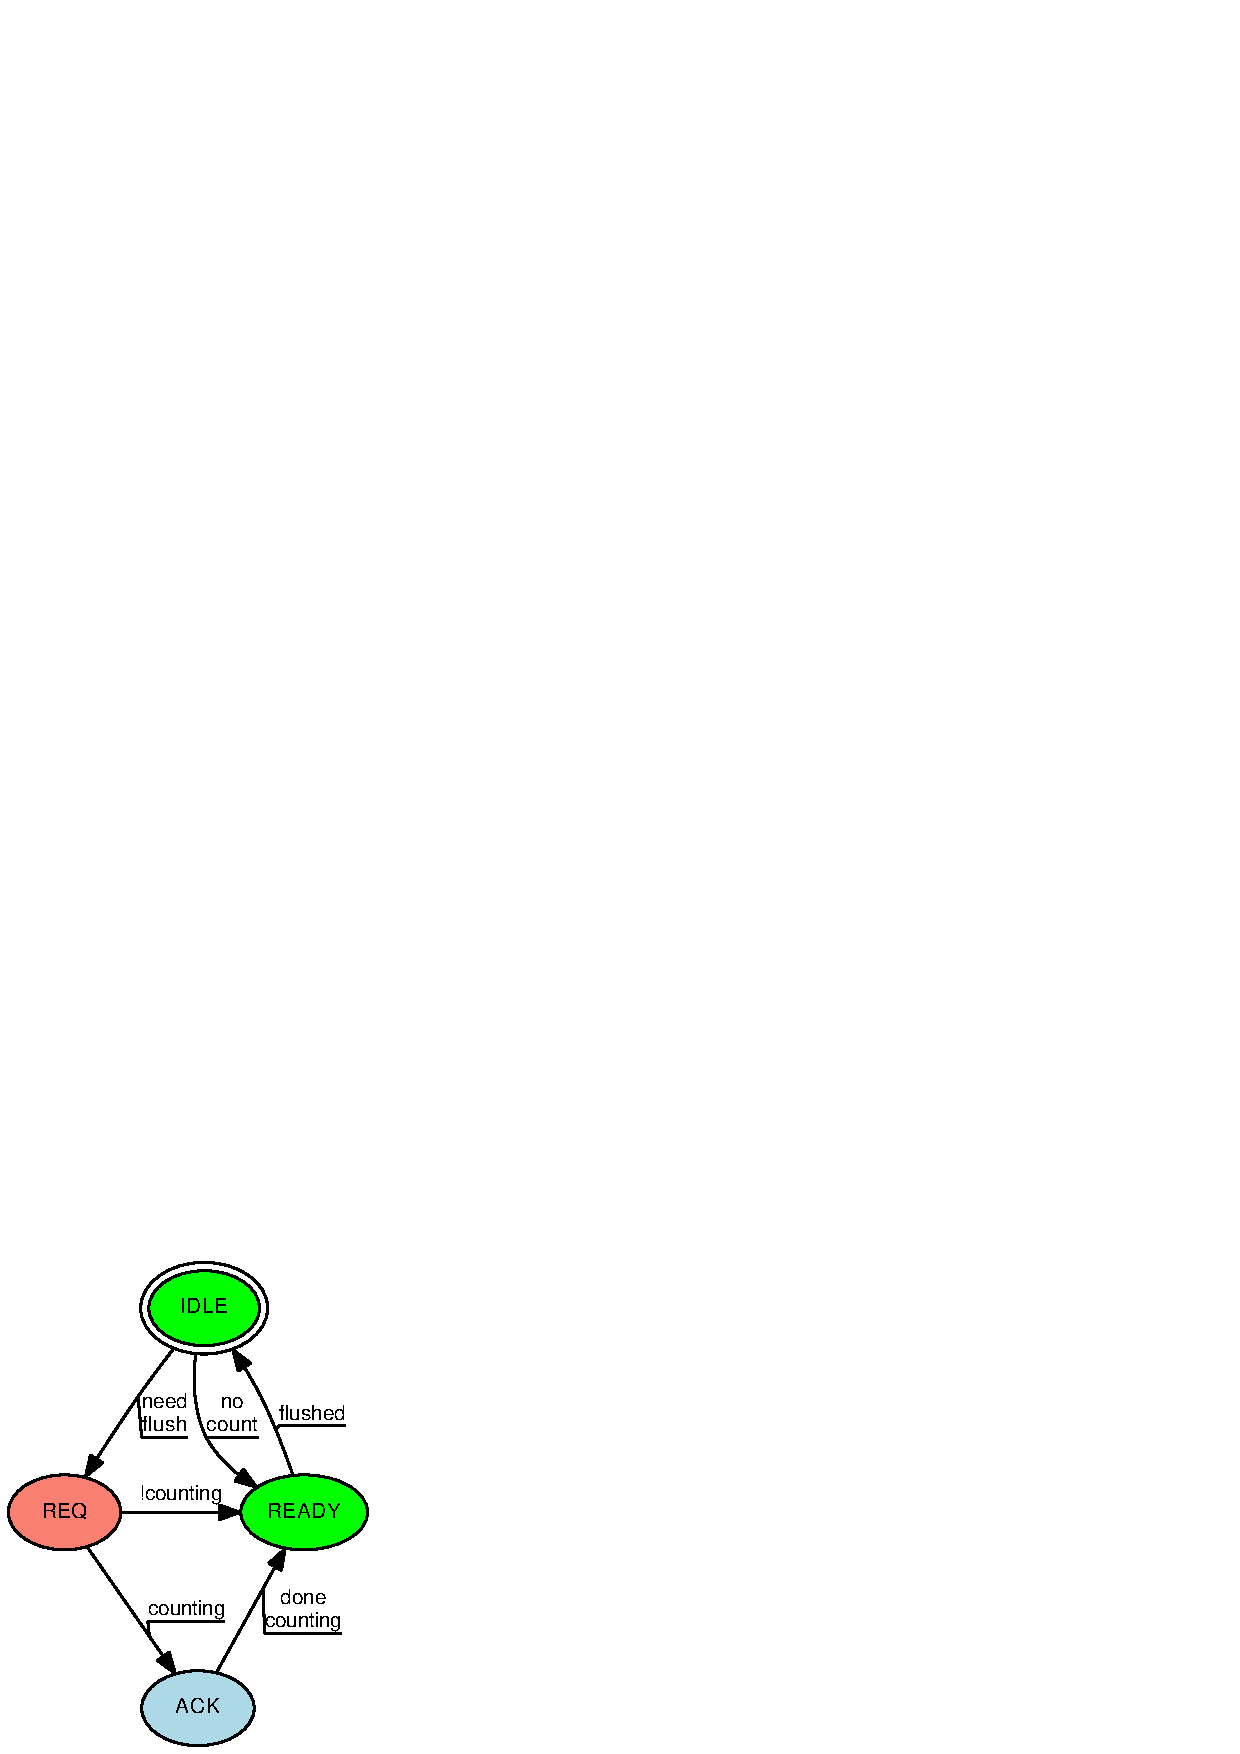
\includegraphics{count/sig-theft}}
\caption{Signal-Theft State Machine}
\label{fig:count:Signal-Theft State Machine}
\end{figure}

쓰레드별 상태는 이제 연관된 쓰레드에 의해서만 조정된다고는 해도, 여전히 시그널
핸들러를 이용해 동기화를 할 필요가 있습니다.
이 동기화는 Figure~\ref{fig:count:Signal-Theft State Machine} 에 보여지는
스테이트 머신에 의해 제공됩니다.
해당 스테이트 머신은 IDLE 상태에서 시작하고 \co{add_count()} 나
\co{sub_count()} 가 로컬 쓰레드의 카운트의 합과 글로벌 카운트가 주어진 요청을
수용할 수 없다는 걸 알았을 때, 관련된 느린 수행 경로는 각 쓰레드의 \co{theft}
상태를 REQ 로 만듭니다 (해당 쓰레드가 카운트가 있을 경우이고, 그렇지 않다면
READY 로 곧바로 변환시킵니다).
초록색으로 표시되어 있듯, \co{gblcnt_mutex} 락을 쥐고 있는 느린 수행경로만이
IDLE 상태로부터의 변환을 할 수 있습니다.\footnote{
	이 책의 흑백 버전을 위해 말해두자면, IDLE 과 READY 는 초록, REQ 는
	빨강, 그리고 ACK 는 파란색으로 되어 있습니다.}
이 느린 수행 경로는 이후 각 쓰레드에 시그널을 보내고, 그에 상응하는 시그널
핸들러들이 연관된 쓰레드의 \co{theft} 와 \co{counting} 변수들을 체크합니다.
만약 \co{theft} 상태가 REQ 가 아니라면 시그널 핸들러는 상태를 바꿀 권한이 없고,
따라서 그냥 리턴합니다.
그렇지 않고, \co{counting} 변수가 값이 있어 현재 쓰레드의 빠른 수행경로가 실행
중이란 것을 알게 된다면, 시그널 핸들러는 \co{theft} 상태를 ACK 로, 그렇지
않다면 READY 로 바꿉니다.
\iffalse

Even though per-thread state will now be manipulated only by the
corresponding thread, there will still need to be synchronization
with the signal handlers.
This synchronization is provided by the state machine shown in
Figure~\ref{fig:count:Signal-Theft State Machine}.
The state machine starts out in the IDLE state, and when \co{add_count()}
or \co{sub_count()} find that the combination of the local thread's count
and the global count cannot accommodate the request, the corresponding
slowpath sets each thread's \co{theft} state to REQ (unless that thread
has no count, in which case it transitions directly to READY).
Only the slowpath, which holds the \co{gblcnt_mutex} lock, is permitted to
transition from the IDLE state, as indicated by the green color.\footnote{
	For those with black-and-white versions of this book,
	IDLE and READY are green, REQ is red, and ACK is blue.}
The slowpath then sends a signal to each thread, and the corresponding
signal handler checks the corresponding thread's \co{theft} and
\co{counting} variables.
If the \co{theft} state is not REQ, then the signal handler is not
permitted to change the state, and therefore simply returns.
Otherwise, if the \co{counting} variable is set, indicating that
the current thread's fastpath is in progress, the signal handler
sets the \co{theft} state to ACK, otherwise to READY.
\fi

파란색으로 표시되어 있듯, \co{theft} 상태가 ACK 라면 빠른 수행 경로만이
\co{theft} 상태를 바꿀 수 있습니다.
빠른 수행 경로가 완료되면, \co{theft} 상태를 READY 로 바꿉니다.

느린 수행 경로가 한 쓰레드의 \co{theft} 상태가 READY 임을 일단 봤다면, 이 느린
수행 경로는 해당 쓰레드의 카운트를 훔칠 권한을 갖습니다.
이 느린 수행 경로는 이후 해당 쓰레드의 \co{theft} 상태를 IDLE 로 만듭니다.
\iffalse

If the \co{theft} state is ACK,
only the fastpath is permitted to change
the \co{theft} state, as indicated by the blue color.
When the fastpath completes, it sets the \co{theft} state to READY.

Once the slowpath sees a thread's \co{theft} state is READY, the
slowpath is permitted to steal that thread's count.
The slowpath then sets that thread's \co{theft} state to IDLE.
\fi

\QuickQuiz{}
	Figure~\ref{fig:count:Signal-Theft State Machine} 에서 REQ \co{theft}
	상태는 왜 빨간색으로 칠해졌나요?
	\iffalse

	In Figure~\ref{fig:count:Signal-Theft State Machine}, why is
	the REQ \co{theft} state colored red?
	\fi
\QuickQuizAnswer{
	빠른 수행 경로만이 \co{theft} 상태를 바꿀 수 있음과 해당 쓰레드가 이
	상태에 너무 오래 머무르면, 느린 수행 경로를 수행하고 있는 쓰레드는
	POSIX 시그널을 다시 보낼 것임을 알리기 위해서입니다.
	\iffalse

	To indicate that only the fastpath is permitted to change the
	\co{theft} state, and that if the thread remains in this
	state for too long, the thread running the slowpath will
	resend the POSIX signal.
	\fi
} \QuickQuizEnd

\QuickQuiz{}
	Figure~\ref{fig:count:Signal-Theft State Machine} 에서, 두개의 분리된
	REQ 와 ACK \co{theft} 상태를 갖는 이유가 뭐죠?
	왜 그 두 상태를 하나의 REQACK 상태로 만들어서 스테이트 머신을 간단하게
	만들지 않는 거예요?
	만약 그렇게 하면 그 상태에 먼저 도달하는 시그널 핸들러나 빠른 수행
	경로가 상태를 READY 로 바꿀 수 있을 텐데요.
	\iffalse

	In Figure~\ref{fig:count:Signal-Theft State Machine}, what is
	the point of having separate REQ and ACK \co{theft} states?
	Why not simplify the state machine by collapsing
	them into a single REQACK state?
	Then whichever of the signal handler or the fastpath gets there
	first could set the state to READY.
	\fi
\QuickQuizAnswer{
	REQ 와 ACK 상태를 합치는게 나쁜 이유를 들어보자면:
	\begin{enumerate}
	\item	해당 느린 수행 경로는 REQ 와 ACK 상태를 사용해 언제 시그널이
		다시 보내져야 할지 결정합니다.
		만약 해당 상태들이 합쳐진다면, 해당 느린 수행 경로는 반복적으로
		시그널을 보내는 수밖에 없고, 빠른 수행경로를 불필요하게 느리게
		만드는 효과를 만들 겁니다.
	\item	다음과 같은 레이스가 일어날 수 있습니다:
		\begin{enumerate}
		\item	느린 수행 경로가 주어진 쓰레드의 상태를 \mbox{REQACK}
			으로 만듭니다.
		\item	해당 쓰레드는 방금 빠른 수행 경로를 끝낸 참이었고,
			REQACK 상태임을 확인합니다.
		\item	해당 쓰레드는 시그널을 받고, 여기서도 REQACK 상태임을
			확인합니다만, 빠른 수행 경로는 아무 효과를 발휘하지
			못한 채이므로, 상태를 READY 로 바꿉니다.
		\item	느린 수행 경로는 READY 상태를 확인하고, 카운트를
			가져가고 상태를 IDLE 로 돌려놓고 완료됩니다.
		\item	빠른 수행 경로는 상태를 READY 로 바꾸고, 이
			쓰레드에서의 다음 빠른 수행 경로 수행을 막아버립니다.
		\end{enumerate}
		여기서의 기본적 문제는 합쳐진 \mbox{REQACK} 상태는 시그널
		핸들러와 빠른 수행 경로 둘 다 볼 수 있다는 겁니다.
		네개의 상태로 관리되는 명확한 분리 상태는 순서화된 상태 전환을
		분명히 보장합니다.
	\end{enumerate}
	\iffalse

	Reasons why collapsing the REQ and ACK states would be a very
	bad idea include:
	\begin{enumerate}
	\item	The slowpath uses the REQ and ACK states to determine
		whether the signal should be retransmitted.
		If the states were collapsed, the slowpath would have
		no choice but to send redundant signals, which would
		have the unhelpful effect of needlessly slowing down
		the fastpath.
	\item	The following race would result:
		\begin{enumerate}
		\item	The slowpath sets a given thread's state to REQACK.
		\item	That thread has just finished its fastpath, and
			notes the REQACK state.
		\item	The thread receives the signal, which also notes
			the REQACK state, and, because there is no fastpath
			in effect, sets the state to READY.
		\item	The slowpath notes the READY state, steals the
			count, and sets the state to IDLE, and completes.
		\item	The fastpath sets the state to READY, disabling
			further fastpath execution for this thread.
		\end{enumerate}
		The basic problem here is that the combined REQACK state
		can be referenced by both the signal handler and the
		fastpath.
		The clear separation maintained by the four-state
		setup ensures orderly state transitions.
	\end{enumerate}
	\fi
	그렇다곤 하지만, 세개의 상태만으로도 제대로 동작하도록 할 수 있을 수도
	있습니다.
	만약 성공하면 네개 상태 버전과 잘 비교해 보세요.
	세개 상태 버전이 정말 더 낫나요, 그리고 왜죠 또는 왜 아니죠?
	\iffalse

	That said, you might well be able to make a three-state setup
	work correctly.
	If you do succeed, compare carefully to the four-state setup.
	Is the three-state solution really preferable, and why or why not?
	\fi
} \QuickQuizEnd

\subsection{Signal-Theft Limit Counter Implementation}
\label{sec:count:Signal-Theft Limit Counter Implementation}

\begin{listing}[tbp]
{ \scriptsize
\begin{verbbox}
  1 #define THEFT_IDLE  0
  2 #define THEFT_REQ   1
  3 #define THEFT_ACK   2
  4 #define THEFT_READY 3
  5 
  6 int __thread theft = THEFT_IDLE;
  7 int __thread counting = 0;
  8 unsigned long __thread counter = 0;
  9 unsigned long __thread countermax = 0;
 10 unsigned long globalcountmax = 10000;
 11 unsigned long globalcount = 0;
 12 unsigned long globalreserve = 0;
 13 unsigned long *counterp[NR_THREADS] = { NULL };
 14 unsigned long *countermaxp[NR_THREADS] = { NULL };
 15 int *theftp[NR_THREADS] = { NULL };
 16 DEFINE_SPINLOCK(gblcnt_mutex);
 17 #define MAX_COUNTERMAX 100
\end{verbbox}
}
\centering
\theverbbox
\caption{Signal-Theft Limit Counter Data}
\label{lst:count:Signal-Theft Limit Counter Data}
\end{listing}

Listing~\ref{lst:count:Signal-Theft Limit Counter Data}
(\path{count_lim_sig.c})
는 signal-theft based counter 구현에 사용되는 데이터 구조를 보입니다.
라인~1-7 에서는 앞의 섹션에서 설명한 쓰레드별 theft 스테이트 머신을 위한 상태와
값들을 정의합니다.
라인~8-17 은 앞의 구현과 비슷합니다만, 라인~14 와 15 에 쓰레드의
\co{countermax} 와 \co{theft} 변수에의 원격에서의 접근을 허가하기 위한 코드가
추가되었습니다.
\iffalse

Listing~\ref{lst:count:Signal-Theft Limit Counter Data}
(\path{count_lim_sig.c})
shows the data structures used by the signal-theft based counter
implementation.
Lines~1-7 define the states and values for the per-thread theft state machine
described in the preceding section.
Lines~8-17 are similar to earlier implementations, with the addition of
lines~14 and~15 to allow remote access to a thread's \co{countermax}
and \co{theft} variables, respectively.
\fi

\begin{listing}[tbp]
{ \scriptsize
\begin{verbbox}
  1 static void globalize_count(void)
  2 {
  3   globalcount += counter;
  4   counter = 0;
  5   globalreserve -= countermax;
  6   countermax = 0;
  7 }
  8 
  9 static void flush_local_count_sig(int unused)
 10 {
 11   if (READ_ONCE(theft) != THEFT_REQ)
 12     return;
 13   smp_mb();
 14   WRITE_ONCE(theft, THEFT_ACK);
 15   if (!counting) {
 16     WRITE_ONCE(theft, THEFT_READY);
 17   }
 18   smp_mb();
 19 }
 20 
 21 static void flush_local_count(void)
 22 {
 23   int t;
 24   thread_id_t tid;
 25 
 26   for_each_tid(t, tid)
 27     if (theftp[t] != NULL) {
 28       if (*countermaxp[t] == 0) {
 29         WRITE_ONCE(*theftp[t], THEFT_READY);
 30         continue;
 31       }
 32       WRITE_ONCE(*theftp[t], THEFT_REQ);
 33       pthread_kill(tid, SIGUSR1);
 34     }
 35   for_each_tid(t, tid) {
 36     if (theftp[t] == NULL)
 37       continue;
 38     while (READ_ONCE(*theftp[t]) != THEFT_READY) {
 39       poll(NULL, 0, 1);
 40       if (READ_ONCE(*theftp[t]) == THEFT_REQ)
 41         pthread_kill(tid, SIGUSR1);
 42     }
 43     globalcount += *counterp[t];
 44     *counterp[t] = 0;
 45     globalreserve -= *countermaxp[t];
 46     *countermaxp[t] = 0;
 47     WRITE_ONCE(*theftp[t], THEFT_IDLE);
 48   }
 49 }
 50 
 51 static void balance_count(void)
 52 {
 53   countermax = globalcountmax -
 54     globalcount - globalreserve;
 55   countermax /= num_online_threads();
 56   if (countermax > MAX_COUNTERMAX)
 57     countermax = MAX_COUNTERMAX;
 58   globalreserve += countermax;
 59   counter = countermax / 2;
 60   if (counter > globalcount)
 61     counter = globalcount;
 62   globalcount -= counter;
 63 }
\end{verbbox}
}
\centering
\theverbbox
\caption{Signal-Theft Limit Counter Value-Migration Functions}
\label{lst:count:Signal-Theft Limit Counter Value-Migration Functions}
\end{listing}

Listing~\ref{lst:count:Signal-Theft Limit Counter Value-Migration Functions}
는 쓰레드별 변수와 전역 변수 사이에 카운트를 옮겨주는 함수를 보입니다.
라인~1-7 은 \co{globalize_count()} 함수를 보이는데, 이 함수는 앞의 구현과
동일합니다.
라인~9-19 는 \co{flush_local_count_sig()} 함수로, 훔치기 과정에서 사용되는
시그널 핸들러입니다.
라인~11 과 12 에서는 \co{theft} 상태가 REQ 인지 확인하고, 아니라면 변경 없이
리턴합니다.
라인~13 에서는 theft 변수의 샘플링이 해당 변수에의 변경 이전에 이루어졌음을
분명히 하기 위해 메모리 배리어를 칩니다.
라인~14 는 \co{theft} 상태를 ACK 로 놓고, 라인~15 에서는 이 쓰레드의 빠른 수행
경로가 수행중인지 확인 후, 라인~16 에서 \co{theft} 상태를 READY 로 놓습니다.
\iffalse

Listing~\ref{lst:count:Signal-Theft Limit Counter Value-Migration Functions}
shows the functions responsible for migrating counts between per-thread
variables and the global variables.
Lines~1-7 shows \co{globalize_count()}, which is identical to earlier
implementations.
Lines~9-19 shows \co{flush_local_count_sig()}, which is the signal
handler used in the theft process.
Lines~11 and~12 check to see if the \co{theft} state is REQ, and, if not
returns without change.
Line~13 executes a memory barrier to ensure that the sampling of the
theft variable happens before any change to that variable.
Line~14 sets the \co{theft} state to ACK, and, if line~15 sees that
this thread's fastpaths are not running, line~16 sets the \co{theft}
state to READY.
\fi

\QuickQuiz{}
	Listing~\ref{lst:count:Signal-Theft Limit Counter Value-Migration Functions}
	의 \co{flush_local_count_sig()} 함수에서는 왜 \co{theft} 쓰레드별
	변수의 사용을 \co{ACCESS_ONCE()} 로 감싼거죠?
	\iffalse

	In Listing~\ref{lst:count:Signal-Theft Limit Counter Value-Migration Functions}
	function \co{flush_local_count_sig()}, why are there
	\co{READ_ONCE()} and \co{WRITE_ONCE()} wrappers around
	the uses of the
	\co{theft} per-thread variable?
	\fi
\QuickQuizAnswer{
	첫번째 \co{ACCESS_ONCE} 사용은 (라인~11) 은 필요 없는 것이라 주장할
	수도 있습니다.
	다음의 두 군데 사용은 (라인~14 와 16) 중요합니다.
	이것들이 없어지면, 컴파일러는 라인~14-17 을 다음과 같이 바꿀 수도
	있습니다:
	\iffalse

	The first one (on line~11) can be argued to be unnecessary.
	The last two (lines~14 and~16) are important.
	If these are removed, the compiler would be within its rights
	to rewrite lines~14-17 as follows:
	\fi

	\vspace{5pt}
	\begin{minipage}[t]{\columnwidth}
	\small
	\begin{verbatim}
 14   theft = THEFT_READY;
 15   if (counting) {
 16     theft = THEFT_ACK;
 17   }
	\end{verbatim}
	\end{minipage}
	\vspace{5pt}
	느린 수행 경로는 잠깐 들어오는 값인 \co{THEFT_READY} 를 보고서 연관된
	쓰레드가 준비되기도 전에 값을 훔쳐가기 시작할테니 위험합니다.
	\iffalse

	This would be fatal, as the slowpath might see the transient
	value of \co{THEFT_READY}, and start stealing before the
	corresponding thread was ready.
	\fi
} \QuickQuizEnd

라인~21-49 는 \co{flush_local_count()} 를 보이는데, 이 함수는 느린 수행
경로에서 모든 쓰레드의 로컬 카운트를 비우기 위해 호출됩니다.
라인~26-34 의 루프에서는 로컬 카운트가 있는 모든 쓰레드의 \co{theft} 상태를
바꾸고, 해당 쓰레드들에 시그널을 날립니다.
라인~27 에서는 존재하지 않는 쓰레드들을 스킵합니다.
그렇지 않다면, 라인~28 에서 현재 쓰레드가 로컬 카운트를 가지고 있는지 보고,
가지고 있지 않다면 라인~29 에서 해당 쓰레드의 \co{theft} 상태를 READY 로 바꾸고
라인~30 에서 다음 쓰레드로 넘어갑니다.
그렇지 않고 현재 쓰레드가 로컬 카운트를 가지고 있다면, 라인~32 에서 해당
쓰레드의 \co{theft} 상태를 REQ 로 바꾸고, 라인~33 에서 시그널을 날립니다.
\iffalse

Lines~21-49 shows \co{flush_local_count()}, which is called from the
slowpath to flush all threads' local counts.
The loop spanning lines~26-34 advances the \co{theft} state for each
thread that has local count, and also sends that thread a signal.
Line~27 skips any non-existent threads.
Otherwise, line~28 checks to see if the current thread holds any local
count, and, if not, line~29 sets the thread's \co{theft} state to READY
and line~30 skips to the next thread.
Otherwise, line~32 sets the thread's \co{theft} state to REQ and
line~33 sends the thread a signal.
\fi

\QuickQuiz{}
	Listing~\ref{lst:count:Signal-Theft Limit Counter Value-Migration
	Functions} 에서, 왜 다른 쓰레드의 \co{countermax} 변수를 바로 접근해도
	안전한 거죠?
	\iffalse

	In Listing~\ref{lst:count:Signal-Theft Limit Counter Value-Migration Functions},
	why is it safe for line~28 to directly access the other thread's
	\co{countermax} variable?
	\fi
\QuickQuizAnswer{
	그 다른 쓰레드는 자신의 \co{countermax} 변수의 값을 \co{gblcnt_mutex}
	락을 쥐지 않은 한 수정할 수 없기 때문입니다.
	하지만 이 함수 호출 코드는 락을 잡고 함수를 호출하기 때문에, 그 다른
	쓰레드는 해당 락을 잡을 수가 없고, 따라서 그 다른 쓰레드는
	\co{countermax} 변수를 수정할 수 없습니다.
	따라서 바로 접근해도 안전합니다---하지만 바꾸진 않습니다.
	\iffalse

	Because the other thread is not permitted to change the value
	of its \co{countermax} variable unless it holds the
	\co{gblcnt_mutex} lock.
	But the caller has acquired this lock, so it is not possible
	for the other thread to hold it, and therefore the other thread
	is not permitted to change its \co{countermax} variable.
	We can therefore safely access it---but not change it.
	\fi
} \QuickQuizEnd

\QuickQuiz{}
	Listing~\ref{lst:count:Signal-Theft Limit Counter Value-Migration Functions}
	에서, 왜 라인~33 은 현재 쓰레드가 자기 자신에게 시그널을 보내는지
	체크하지 않나요?
	\iffalse

	In Listing~\ref{lst:count:Signal-Theft Limit Counter Value-Migration Functions},
	why doesn't line~33 check for the current thread sending itself
	a signal?
	\fi
\QuickQuizAnswer{
	또한번 체크할 필요가 없습니다.
	\co{flush_local_count()} 는 이미 \co{globalize_count()} 를 호출했으니,
	라인~28 에서의 체크가 성공해서 뒤의 \co{pthread_kill()} 은 스킵될
	겁니다.
	\iffalse

	There is no need for an additional check.
	The caller of \co{flush_local_count()} has already invoked
	\co{globalize_count()}, so the check on line~28 will have
	succeeded, skipping the later \co{pthread_kill()}.
	\fi
} \QuickQuizEnd

\QuickQuiz{}
	Listing~\ref{lst:count:Signal-Theft Limit Counter Value-Migration Functions}
	의 코드는 \GCC\ 와 POSIX 에서 동작합니다.
	ISO C 표준에서 동작하게 하려면 뭐가 필요할까요?
	\iffalse

	The code in
	Listing~\ref{lst:count:Signal-Theft Limit Counter Value-Migration Functions},
	works with \GCC\ and POSIX.
	What would be required to make it also conform to the ISO C standard?
	\fi
\QuickQuizAnswer{
	\co{theft} 변수는 안전하게 시그널 핸들러와 시그널에 인터럽트되는 코드
	사이에서 안전하게 공유될 수 있도록 \co{sig_atomic_t} 타입이어야만
	합니다.
	\iffalse

	The \co{theft} variable must be of type \co{sig_atomic_t}
	to guarantee that it can be safely shared between the signal
	handler and the code interrupted by the signal.
	\fi
} \QuickQuizEnd

라인~35-48 의 루프는 각 쓰레드가 READY 상태에 도달하길 기다리고, 이후 해당
쓰레드의 카운트를 훔칩니다.
라인~36-37 은 존재하지 않는 쓰레드들을 스킵하고, 라인~38-42 의 루프에서 현재
쓰레드의 \co{theft} 상태가 READY 가 되길 기다립니다.
라인~39 에서는 우선순위 역전(priority-inversion) 문제를 막기 위해 1 밀리세컨드
동안 블락되고, 라인~40 에서 해당 쓰레드의 시그널이 아직 도착하지 않은 것으로
판단되면 라인~41 에서 시그널을 다시 날립니다.
현재 살펴보고 있는 쓰레드의 상태가 마침내 READY 가 되면 실행 흐름은 라인~43 에
도달해 라인~43-46 에서 훔치기를 시전합니다.
라인~47 은 해당 쓰레드의 \co{theft} 상태를 다시 IDLE 로 되돌립니다.
\iffalse

The loop spanning lines~35-48 waits until each thread reaches READY state,
then steals that thread's count.
Lines~36-37 skip any non-existent threads, and the loop spanning
lines~38-42 wait until the current thread's \co{theft} state becomes READY.
Line~39 blocks for a millisecond to avoid priority-inversion problems,
and if line~40 determines that the thread's signal has not yet arrived,
line~41 resends the signal.
Execution reaches line~43 when the thread's \co{theft} state becomes
READY, so lines~43-46 do the thieving.
Line~47 then sets the thread's \co{theft} state back to IDLE.
\fi

\QuickQuiz{}
	Listing~\ref{lst:count:Signal-Theft Limit Counter Value-Migration Functions}
	의 라인~41 에서는 왜 시그널을 다시 보내죠?
	\iffalse

	In Listing~\ref{lst:count:Signal-Theft Limit Counter Value-Migration Functions}, why does line~41 resend the signal?
	\fi
\QuickQuizAnswer{
	지난 수십년간 많은 운영 체제는 갑자기 시그널을 잃어버리는 특성을 가졌기
	때문입니다.
	이게 기능인지 버그인지는 논쟁거리이지만, 그건 무의미합니다.
	사용자가 보기에 분명한 증상은 커널 버그가 아니라 사용자
	어플리케이션의 문제입니다.

	\emph{당신의} 어플리케이션의 문제입니다!
	\iffalse

	Because many operating systems over several decades have
	had the property of losing the occasional signal.
	Whether this is a feature or a bug is debatable, but
	irrelevant.
	The obvious symptom from the user's viewpoint will not be
	a kernel bug, but rather a user application hanging.

	\emph{Your} user application hanging!
	\fi
} \QuickQuizEnd

라인~51-63 에서는 \co{balance_count()} 함수를 보이는데, 앞의 예제와 비슷합니다.
\iffalse

Lines~51-63 show \co{balance_count()}, which is similar to that of
earlier examples.
\fi

\begin{listing}[tbp]
{ \scriptsize
\begin{verbbox}
  1 int add_count(unsigned long delta)
  2 {
  3   int fastpath = 0;
  4 
  5   counting = 1;
  6   barrier();
  7   if (countermax - counter >= delta &&
  8       READ_ONCE(theft) <= THEFT_REQ) {
  9     counter += delta;
 10     fastpath = 1;
 11   }
 12   barrier();
 13   counting = 0;
 14   barrier();
 15   if (READ_ONCE(theft) == THEFT_ACK) {
 16     smp_mb();
 17     WRITE_ONCE(theft, THEFT_READY);
 18   }
 19   if (fastpath)
 20     return 1;
 21   spin_lock(&gblcnt_mutex);
 22   globalize_count();
 23   if (globalcountmax - globalcount -
 24       globalreserve < delta) {
 25     flush_local_count();
 26     if (globalcountmax - globalcount -
 27         globalreserve < delta) {
 28       spin_unlock(&gblcnt_mutex);
 29       return 0;
 30     }
 31   }
 32   globalcount += delta;
 33   balance_count();
 34   spin_unlock(&gblcnt_mutex);
 35   return 1;
 36 }
\end{verbbox}
}
\centering
\theverbbox
\caption{Signal-Theft Limit Counter Add Function}
\label{lst:count:Signal-Theft Limit Counter Add Function}
\end{listing}

\begin{listing}[tb]
{ \scriptsize
\begin{verbbox}
 38 int sub_count(unsigned long delta)
 39 {
 40   int fastpath = 0;
 41 
 42   counting = 1;
 43   barrier();
 44   if (counter >= delta &&
 45       READ_ONCE(theft) <= THEFT_REQ) {
 46     counter -= delta;
 47     fastpath = 1;
 48   }
 49   barrier();
 50   counting = 0;
 51   barrier();
 52   if (READ_ONCE(theft) == THEFT_ACK) {
 53     smp_mb();
 54     WRITE_ONCE(theft, THEFT_READY);
 55   }
 56   if (fastpath)
 57     return 1;
 58   spin_lock(&gblcnt_mutex);
 59   globalize_count();
 60   if (globalcount < delta) {
 61     flush_local_count();
 62     if (globalcount < delta) {
 63       spin_unlock(&gblcnt_mutex);
 64       return 0;
 65     }
 66   }
 67   globalcount -= delta;
 68   balance_count();
 69   spin_unlock(&gblcnt_mutex);
 70   return 1;
 71 }
\end{verbbox}
}
\centering
\theverbbox
\caption{Signal-Theft Limit Counter Subtract Function}
\label{lst:count:Signal-Theft Limit Counter Subtract Function}
\end{listing}

Listing~\ref{lst:count:Signal-Theft Limit Counter Add Function} 는
\co{add_count()} 함수를 보입니다.
라인~5-20 에는 빠른 수행 경로가, 라인~21-35 에는 느린 수행 경로가 있습니다.
라인~5 에서는 쓰레드별 \co{counting} 변수를 1로 만들어서 이후에 이 쓰레드를
인터럽트하는 어떤 시그널 핸들러도 \co{theft} 상태를 READY 가 아니라 ACK 로
설정하게 해둠으로써, 이 빠른 수행 경로가 올바르게 완료되도록 합니다.
라인~6 은 컴파일러가 빠른 수행 경로의 본체가 \co{counting} 설정보다 앞에
위치하도록 재배치 하는 것을 막아줍니다.
라인~7 과 8 은 쓰레드별 데이터가 \co{add_count()} 를 처리할 수 있는지 확인하고
현재 수행중인 훔치기 작업이 없다면 라인~9 에서 빠른 수행 경로 더하기 연산을
수행하고 라인~10 에서 빠른 수행 경로가 진행됨을 알립니다.
\iffalse

Listing~\ref{lst:count:Signal-Theft Limit Counter Add Function}
shows the \co{add_count()} function.
The fastpath spans lines~5-20, and the slowpath lines~21-35.
Line~5 sets the per-thread \co{counting} variable to 1 so that
any subsequent signal handlers interrupting this thread will
set the \co{theft} state to ACK rather than READY, allowing this
fastpath to complete properly.
Line~6 prevents the compiler from reordering any of the fastpath body
to precede the setting of \co{counting}.
Lines~7 and~8 check to see if the per-thread data can accommodate
the \co{add_count()} and if there is no ongoing theft in progress,
and if so line~9 does the fastpath addition and line~10 notes that
the fastpath was taken.
\fi

어떤 경우든, 라인~12 에서 컴파일러가 빠른 수행 경로 본체가 라인~13 뒤에 오도록
재배치해 이후의 시그널 핸들러가 훔치기 작업을 하는 사태를 만들지 못하게 합니다.
라인~14 에서는 다시 컴파일러 재배치를 막고, 라인~15 에서 시그널 핸들러가
\co{theft} 상태를 READY 로 바꿨는지 보고, 만약 그렇다면 라인~16 에서 라인~17
에서 READY 로 설정한 상태를 본 CPU 는 라인~9 의 결과도 보도록 해줍니다.
라인~9 에서의 빠른 수행 경로 더하기가 실행되었다면, 라인~20 에서 성공을
리턴합니다.
\iffalse

In either case, line~12 prevents the compiler from reordering the
fastpath body to follow line~13, which permits any subsequent signal
handlers to undertake theft.
Line~14 again disables compiler reordering, and then line~15
checks to see if the signal handler deferred the \co{theft}
state-change to READY, and, if so, line~16 executes a memory
barrier to ensure that any CPU that sees line~17 setting state to
READY also sees the effects of line~9.
If the fastpath addition at line~9 was executed, then line~20 returns
success.
\fi

\begin{listing}[tbp]
{ \scriptsize
\begin{verbbox}
  1 unsigned long read_count(void)
  2 {
  3   int t;
  4   unsigned long sum;
  5 
  6   spin_lock(&gblcnt_mutex);
  7   sum = globalcount;
  8   for_each_thread(t)
  9     if (counterp[t] != NULL)
 10       sum += *counterp[t];
 11   spin_unlock(&gblcnt_mutex);
 12   return sum;
 13 }
\end{verbbox}
}
\centering
\theverbbox
\caption{Signal-Theft Limit Counter Read Function}
\label{lst:count:Signal-Theft Limit Counter Read Function}
\end{listing}

그렇지 않다면, 라인~21 부터 시작되는 느린 수행 경로로 떨어집니다.
느린 수행 경로의 구조는 앞의 예제들과 유사하므로, 분석은 독자 여러분의 연습
문제로 놔두겠습니다.
비슷하게, Listing~\ref{lst:count:Signal-Theft Limit Counter Subtract Function}
의 \co{sub_count()} 의 구조는 \co{add_count()} 와 동일하므로, \co{sub_count()}
역시, 그리고 Listing~\ref{lst:count:Signal-Theft Limit Counter Read Function}
의 \co{read_count()} 와 함께 그 분석을 독자 여러분의 몫으로 남겨 두겠습니다.
\iffalse

Otherwise, we fall through to the slowpath starting at line~21.
The structure of the slowpath is similar to those of earlier examples,
so its analysis is left as an exercise to the reader.
Similarly, the structure of \co{sub_count()} on
Listing~\ref{lst:count:Signal-Theft Limit Counter Subtract Function}
is the same
as that of \co{add_count()}, so the analysis of \co{sub_count()} is also
left as an exercise for the reader, as is the analysis of
\co{read_count()} in
Listing~\ref{lst:count:Signal-Theft Limit Counter Read Function}.
\fi

\begin{listing}[tbp]
{ \scriptsize
\begin{verbbox}
  1 void count_init(void)
  2 {
  3   struct sigaction sa;
  4 
  5   sa.sa_handler = flush_local_count_sig;
  6   sigemptyset(&sa.sa_mask);
  7   sa.sa_flags = 0;
  8   if (sigaction(SIGUSR1, &sa, NULL) != 0) {
  9     perror("sigaction");
 10     exit(-1);
 11   }
 12 }
 13 
 14 void count_register_thread(void)
 15 {
 16   int idx = smp_thread_id();
 17 
 18   spin_lock(&gblcnt_mutex);
 19   counterp[idx] = &counter;
 20   countermaxp[idx] = &countermax;
 21   theftp[idx] = &theft;
 22   spin_unlock(&gblcnt_mutex);
 23 }
 24 
 25 void count_unregister_thread(int nthreadsexpected)
 26 {
 27   int idx = smp_thread_id();
 28 
 29   spin_lock(&gblcnt_mutex);
 30   globalize_count();
 31   counterp[idx] = NULL;
 32   countermaxp[idx] = NULL;
 33   theftp[idx] = NULL;
 34   spin_unlock(&gblcnt_mutex);
 35 }
\end{verbbox}
}
\centering
\theverbbox
\caption{Signal-Theft Limit Counter Initialization Functions}
\label{lst:count:Signal-Theft Limit Counter Initialization Functions}
\end{listing}

Listing~\ref{lst:count:Signal-Theft Limit Counter Initialization Functions}
의 라인~1-12 는 \co{count_init()} 를 보여주는데, 이 함수에선
\co{flush_local_count_sig()} 를 \co{SIGUSR1} 의 시그널 핸들러로 설정해서
\co{flush_local_count()} 에서 \co{pthread_kill()} 호출로
\co{flush_local_count_sig()} 를 실행시킬 수 있게 합니다.
쓰레드 등록과 해제를 위한 코드는 앞의 예제와 비슷하므로, 이 코드의 분석은
독자의 몫으로 남겨 두겠습니다.
\iffalse

Lines~1-12 of
Listing~\ref{lst:count:Signal-Theft Limit Counter Initialization Functions}
show \co{count_init()}, which set up \co{flush_local_count_sig()}
as the signal handler for \co{SIGUSR1},
enabling the \co{pthread_kill()} calls in \co{flush_local_count()}
to invoke \co{flush_local_count_sig()}.
The code for thread registry and unregistry is similar to that of
earlier examples, so its analysis is left as an exercise for the
reader.
\fi

\subsection{Signal-Theft Limit Counter Discussion}

Signal-theft 구현은 제 Intel Core Duo 랩탑에서 어토믹 인스트럭션 구현보다 두배
이상 빠르게 동작합니다.
항상 그럴까요?

Signal-theft 구현은 펜티엄-4 시스템에서는 어토믹 인스트럭션들이 느리기 때문에
선호될만 합니다만 과거의 80386 기반 Sequent Symmetry 시스템에서는 어토믹
오퍼레이션을 사용한 구현의 더 짧은 코드를 더 빨리 수행할 것입니다.
하지만, 이 업데이트 쪽의 성능 향상은 읽는 쪽의 높아진 오버헤드와 함께 옵니다:
POSIX 시그널은 공짜가 아닙니다.
결국 핵심이 성능이라면, 두 구현 모두를 어플리케이션이 배포될 시스템 위에서
돌려보는게 좋을 겁니다.
\iffalse

The signal-theft implementation runs more than twice as fast as the
atomic implementation on my Intel Core Duo laptop.
Is it always preferable?

The signal-theft implementation would be vastly preferable on Pentium-4
systems, given their slow atomic instructions, but the old 80386-based
Sequent Symmetry systems would do much better with the shorter path
length of the atomic implementation.
However, this increased update-side performance comes at the
prices of higher read-side overhead: Those POSIX signals are not free.
If ultimate performance is of the essence, you will need to measure
them both on the system that your application is to be deployed on.
\fi

\QuickQuiz{}
	POSIX 시그널만 느린게 아니라, 시그널을 각 쓰레드에 보내는 행위 자체가
	확장성이 없어요.
	만약 10,000 개의 쓰레드가 있고 읽는 쪽도 빨라야 한다면 어떻게
	하시겠어요?
	\iffalse

	Not only are POSIX signals slow, sending one to each thread
	simply does not scale.
	What would you do if you had (say) 10,000 threads and needed
	the read side to be fast?
	\fi
\QuickQuizAnswer{
	한가지 방법은
	Section~\ref{sec:count:Eventually Consistent Implementation} 에서
	보였던, 한개의 카운터 변수에 추정치를 합하는 방법입니다.
	또다른 방법으로는 각각 업데이트를 하는 쓰레드의 일부와 상호작용하면서
	읽기 작업을 함께 하는 복수의 쓰레드를 사용하는 방법도 있겠습니다.
	\iffalse

	One approach is to use the techniques shown in
	Section~\ref{sec:count:Eventually Consistent Implementation},
	summarizing an approximation to the overall counter value in
	a single variable.
	Another approach would be to use multiple threads to carry
	out the reads, with each such thread interacting with a
	specific subset of the updating threads.
	\fi
} \QuickQuizEnd

이건 왜 높은 품질의 API 가 그렇게 중요한지를 보여주는 한가지 예이기도 합니다:
높은 품질의 API 는 바뀌는 하드웨어 성능 특성에 따라 요구되는 구현 변경이
가능하게 해줍니다.
\iffalse

This is but one reason why high-quality APIs are so important:
they permit implementations to be changed as required by ever-changing
hardware performance characteristics.
\fi

\QuickQuiz{}
	아래쪽 한계는 명확하게 지키지만 위쪽 한계는 좀 정확하지 않아도 되는
	한계 카운터를 원한다면 어떻게 하면 될까요?
	\iffalse

	What if you want an exact limit counter to be exact only for
	its lower limit, but to allow the upper limit to be inexact?
	\fi
\QuickQuizAnswer{
	한가지 간단한 해결책은 위쪽 한계를 원하는 만큼 더 높게 잡아주는
	것입니다.
	그렇게 더 높게 리미트를 잡아주는 것의 한계는 카운터가 표현할 수 있는
	최대의 값이 될 것입니다.
	\iffalse

	One simple solution is to overstate the upper limit by the
	desired amount.
	The limiting case of such overstatement results in the
	upper limit being set to the largest value that the counter is
	capable of representing.
	\fi
} \QuickQuizEnd

\section{Applying Specialized Parallel Counters}
\label{sec:count:Applying Specialized Parallel Counters}

Section~\ref{sec:count:Exact Limit Counters} 에서 소개한 정확한 리미트 카운터
구현은 매우 유용할 수 있지만, 예를 들어 I/O 디바이스로의 액세스 수를 세는
경우와 같이 카운터의 값이 항상 0에 가깝게 유지된다면 별로 유용하지 않을 겁니다.
그런 경우에서의 높은 오버헤드는 일반적으로 얼마나 많은 레퍼런스들이 존재하는지
신경쓰지 않는다는 점을 감안하면 특히나 큰 문제가 됩니다.
{\QcountQIOcnt} 에서 이야기한, 제거 가능한 I/O 디바이스 액세스 카운트 문제에서
이야기 했듯, 액세스의 갯수는 누군가가 정말로 해당 디바이스를 제거하려 하고 있는
드문 경우가 아니고는 무의미합니다.

이 문제에 대한 간단한 해결책은 카운터에 커다란 ``바이어스'' (예를 들어, 10억
정도) 를 더해 값이 0 보다 충분히 커서 카운터가 효과적으로 동작할 수 있도록
보장해 주는 것입니다.
누군가가 디바이스를 제거하려 한다면, 이 바이어스 값이 카운터 값에서 빠집니다.
마지막의 몇개 액세스들을 카운팅 하는 건 매우 비효율적이 되겠지만, 중요한 건, 그
앞의 많은 액세스들은 최대 속도로 카운트 될 것이라는 점입니다.
\iffalse

Although the exact limit counter implementations in
Section~\ref{sec:count:Exact Limit Counters}
can be very useful, they are not much help if the counter's value
remains near zero at all times, as it might when counting the number
of outstanding accesses to an I/O device.
The high overhead of such near-zero counting is especially painful
given that we normally don't care how many references there are.
As noted in the removable I/O device access-count problem posed by
\QuickQuizRef{\QcountQIOcnt},
the number of accesses is irrelevant except in those rare cases when
someone is actually trying to remove the device.

One simple solution to this problem is to add a large ``bias''
(for example, one billion) to the
counter in order to ensure that the value is far enough from zero that
the counter can operate efficiently.
When someone wants to remove the device, this bias is subtracted from
the counter value.
Counting the last few accesses will be quite inefficient,
but the important point is that the many prior accesses will have been
counted at full speed.
\fi

\QuickQuiz{}
	바이어스된 카운터를 사용할 때 그 외에 뭘 하면 좋을까요?
	\iffalse

	What else had you better have done when using a biased counter?
	\fi
\QuickQuizAnswer{
	카운터가 액세스의 수가 최대값에 가까울 때에도 효과적으로 동작할 수
	있도록 위쪽 리미트를 바이어스, 예상되는 최대 액세스 수, 그리고 충분한
	``출렁거림'' 을 수용하기 충분하도록 크게 잡는게 좋을 겁니다.
	\iffalse

	You had better have set the upper limit to be large enough
	accommodate the bias, the expected maximum number of accesses,
	and enough ``slop'' to allow the counter to work efficiently
	even when the number of accesses is at its maximum.
	\fi
} \QuickQuizEnd

바이어스된 카운터는 매우 유용하고 도움이 될 수 있지만,
page~\pageref{chp:Counting} 에서 이야기된 제거 가능한 I/O 디바이스 액세스
카운트 문제의 부분적 해결책에 불과합니다.
디바이스를 제거하려 시도할 때, 우린 현재 I/O 액세스들의 정확한 갯수를 알아야
할뿐만 아니라, 이후의 액세스가 발생하지 않도록 막아야 합니다.
이걸 해내는 한가지 방법은 리더-라이터 락을 사용해 카운터를 업데이트 할 때 읽기
권한을 획득하고, 카운터를 체크할 때 같은 리더-라이터 락에서 쓰기 권한을
획득하는 것입니다.
I/O 를 위한 코드는 다음과 같이 될겁니다:
\iffalse

Although a biased counter can be quite helpful and useful, it is only a
partial solution to the removable I/O device access-count problem
called out on
page~\pageref{chp:Counting}.
When attempting to remove a device, we must not only know the precise
number of current I/O accesses, we also need to prevent any future
accesses from starting.
One way to accomplish this is to read-acquire a reader-writer lock
when updating the counter, and to write-acquire that same reader-writer
lock when checking the counter.
Code for doing I/O might be as follows:
\fi

\vspace{5pt}
\begin{minipage}[t]{\columnwidth}
\small
\begin{verbatim}
  1 read_lock(&mylock);
  2 if (removing) {
  3   read_unlock(&mylock);
  4   cancel_io();
  5 } else {
  6   add_count(1);
  7   read_unlock(&mylock);
  8   do_io();
  9   sub_count(1);
 10 }
\end{verbatim}
\end{minipage}
\vspace{5pt}

라인~1 에서 락을 이용해 읽기 권한을 획득하고, 라인~3 이나~7 에서 이를
해제합니다.
라인~2 에서는 디바이스가 삭제되는 중인지 확인하고, 그렇다면 라인~3 에서 락을
해제하고 라인~4 에서 I/O 를 취소하거나, 디바이스가 삭제될 예정일 때 해야 할
무슨 일이든 합니다.
디바이스가 삭제중인지 않다면 라인~6 에서 액세스 카운트를 증가시키고 라인~7 에서
락을 해제하고, 라인~8 에서 I/O를 수행한 후, 라인~9 에서 액세스 카운트를
낮춥니다.
\iffalse

Line~1 read-acquires the lock, and either line~3 or~7 releases it.
Line~2 checks to see if the device is being removed, and, if so,
line~3 releases the lock and line~4 cancels the I/O, or takes whatever
action is appropriate given that the device is to be removed.
Otherwise, line~6 increments the access count, line~7 releases the
lock, line~8 performs the I/O, and line~9 decrements the access count.
\fi

\QuickQuiz{}
	이거 참 웃기네요!
	카운터를 \emph{업데이트} 하기 위해 리더-라이터 락의 \emph{읽기} 권한
	획득을 한다니요?
	뭐하는거예요???
	\iffalse

	This is ridiculous!
	We are \emph{read}-acquiring a reader-writer lock to
	\emph{update} the counter?
	What are you playing at???
	\fi
\QuickQuizAnswer{
	이상해 보일 수 있겠죠, 하지만 진짜예요!
	``리더-라이터 락'' 이라는 이름은 사실 완벽하게 의미를 설명하지 못한다는
	점을 상기하면 이해가 될 거예요, 그렇죠?
	\iffalse

	Strange, perhaps, but true!
	Almost enough to make you think that the name
	``reader-writer lock'' was poorly chosen, isn't it?
	\fi
} \QuickQuizEnd

디바이스를 제거하는 코드는 다음과 같을 겁니다:
\iffalse

The code to remove the device might be as follows:
\fi

\vspace{5pt}
\begin{minipage}[t]{\columnwidth}
\small
\begin{verbatim}
  1 write_lock(&mylock);
  2 removing = 1;
  3 sub_count(mybias);
  4 write_unlock(&mylock);
  5 while (read_count() != 0) {
  6   poll(NULL, 0, 1);
  7 }
  8 remove_device();
\end{verbatim}
\end{minipage}
\vspace{5pt}

라인~1 에서는 락의 쓰기-획득을 하고 라인~4 에서 해제합니다.
라인~2 에서 디바이스가 제거되는 중임을 알리고, 라인~5-7 에서 존재하는 I/O
오퍼레이션들이 끝나길 기다립니다.
마지막으로, 라인~8 에서 디바이스 제거에 필요한 작업을 진행합니다.
\iffalse

Line~1 write-acquires the lock and line~4 releases it.
Line~2 notes that the device is being removed, and the loop spanning
lines~5-7 wait for any I/O operations to complete.
Finally, line~8 does any additional processing needed to prepare for
device removal.
\fi

\QuickQuiz{}
	실제 시스템에 적용하려면 해결해야할 문제들이 또 뭐가 있을 수 있을까요?
	\iffalse

	What other issues would need to be accounted for in a real system?
	\fi
\QuickQuizAnswer{
	엄청나게 많습니다!

	일단 몇가지 생각을 시작할 것들은:

	\begin{enumerate}
	\item	디바이스는 여러개가 있을 수 있으니, 전역 변수는 적절치 못하고,
		\co{do_io()}  에 인자가 없는 것도 마찬가지죠.
	\item	폴링하는 루프는 실제 시스템에서는 문제가 있을 수 있습니다.
		많은 경우, 마지막으로 I/O 를 완료 하는 쪽에서 디바이스 제거
		쓰레드를 깨우는 편이 낫습니다.
	\item	I/O 는 실패할 수 있으므로, \co{do_io()} 는 리턴 값을 가져야 할
		겁니다.
	\item	디바이스가 고장나면, 마지막 I/O 는 성공하지 못할 것입니다.
		이런 경우, 에러 복구를 위한 어떤 타임아웃 같은 것이 필요할
		것입니다.
	\item	\co{add_count()} 와 \co{sub_count()} 모두 실패할 수 있는데
		리턴값을 체크하지 않았습니다.
	\item	리더-라이터 락은 확장성이 그다지 좋지 않습니다.
		리더-라이터 락의 읽기 권한 획득의 높은 비용을 회피하는 방법
		한가지가 Chapter~\ref{chp:Locking} 와
		\ref{chp:Deferred Processing} 에 소개되어 있습니다.
	\item	폴링 루프는 매우 낮은 에너지 효율성을 초래할 것입니다.
		이벤트 기반 설계가 나을 겁니다.
	\end{enumerate}
	\iffalse

	A huge number!

	Here are a few to start with:

	\begin{enumerate}
	\item	There could be any number of devices, so that the
		global variables are inappropriate, as are the
		lack of arguments to functions like \co{do_io()}.
	\item	Polling loops can be problematic in real systems.
		In many cases, it is far better to have the last
		completing I/O wake up the device-removal thread.
	\item	The I/O might fail, and so \co{do_io()} will likely
		need a return value.
	\item	If the device fails, the last I/O might never complete.
		In such cases, there might need to be some sort of
		timeout to allow error recovery.
	\item	Both \co{add_count()} and \co{sub_count()} can
		fail, but their return values are not checked.
	\item	Reader-writer locks do not scale well.
		One way of avoiding the high read-acquisition costs
		of reader-writer locks is presented in
		Chapters~\ref{chp:Locking}
		and~\ref{chp:Deferred Processing}.
	\item	The polling loops result in poor energy efficiency.
		An event-driven design is preferable.
	\end{enumerate}
	\fi
} \QuickQuizEnd

\section{Parallel Counting Discussion}
\label{sec:count:Parallel Counting Discussion}

이 챕터에서는 전통적인 카운팅 도구들의 신뢰성, 성능, 그리고 확장성 문제를
보았습니다.
C 언어의 \co{++} 오퍼레이터는 멀티쓰레드 코드에서 신뢰성 있게 동작함을 보장하지
않고, 하나의 변수에 어토믹 오퍼레이션을 행하는 것은 성능도 떨어지고 확장성도
좋지 않습니다.
그래서 이 챕터에서는 일부 특정한 경우에 성능도 좋고 확장성도 매우 좋은 카운팅
알고리즘 일부를 보았습니다.

이 카운팅 알고리즘들에서 얻은 교훈을 리뷰해 보는 것은 가치있는 일일 것입니다.
그러기 위해,
Section~\ref{sec:count:Parallel Counting Performance} 에서 성능과 확장성을
정리하고,
Section~\ref{sec:count:Parallel Counting Specializations} 에서 특수화를 위한
필요성을 이야기해 보고,
그리고 마지막으로
Section~\ref{sec:count:Parallel Counting Lessons} 에서 이번에 배운 교훈들을
나열해보고 이 교훈들로부터 더 나아갈 뒤의 챕터에 대해 간단히 알아봅니다.
\iffalse

This chapter has presented the reliability, performance, and
scalability problems with traditional counting primitives.
The C-language \co{++} operator is not guaranteed to function reliably in
multithreaded code, and atomic operations to a single variable neither
perform nor scale well.
This chapter therefore presented a number of counting algorithms that
perform and scale extremely well in certain special cases.

It is well worth reviewing the lessons from these counting algorithms.
To that end,
Section~\ref{sec:count:Parallel Counting Performance}
summarizes performance and scalability,
Section~\ref{sec:count:Parallel Counting Specializations}
discusses the need for specialization,
and finally,
Section~\ref{sec:count:Parallel Counting Lessons}
enumerates lessons learned and calls attention to later chapters that
will expand on these lessons.
\fi

\subsection{Parallel Counting Performance}
\label{sec:count:Parallel Counting Performance}

\begin{table*}
\rowcolors{4}{}{lightgray}
\renewcommand*{\arraystretch}{1.1}
\small
\centering
\begin{tabular}{lrS[table-format = 2.1]S[table-format = 3.0]S[table-format = 5.0]}
	\toprule
	& & & \multicolumn{2}{c}{Reads (ns)} \\
	\cmidrule{4-5}
	Algorithm & Section & \multicolumn{1}{r}{Updates (ns)} &
				    \multicolumn{1}{r}{1 Core} &
					\multicolumn{1}{r}{32 Cores} \\
        \midrule
	\path{count_stat.c} & \ref{sec:count:Array-Based Implementation} &
		11.5 & 408 &    409 \\
	\path{count_stat_eventual.c} & \ref{sec:count:Eventually Consistent Implementation} &
		11.6 &   1 &      1 \\
	\path{count_end.c} & \ref{sec:count:Per-Thread-Variable-Based Implementation} &
		 6.3 & 389 & 51 200 \\
	\path{count_end_rcu.c} & \ref{sec:together:RCU and Per-Thread-Variable-Based Statistical Counters} &
		 5.7 & 354 &    501 \\
	\bottomrule
\end{tabular}
\caption{Statistical Counter Performance on \Power{6}}
\label{tab:count:Statistical Counter Performance on Power-6}
\end{table*}

Table~\ref{tab:count:Statistical Counter Performance on Power-6} 에 네개의 병렬
통계성 카운팅 알고리즘의 성능이 나열되어 있습니다.
네개의 알고리즘 모두 업데이트에 있어 완벽에 가까운 선형적 확장성을 제공합니다.
쓰레드별 변수 구현 (\path{count_end.c}) 는 특히나 어레이 기반
구현(\path{count_stat.c}) 에 비해 업데이트가 빠릅니다만, 코어의 수가 많을 때
읽기 쪽에선 느리며, 많은 읽기 오퍼레이션이 병렬적으로 수행될 때에는 상당한 락
경쟁 상황으로 성능이 떨어집니다.
이 경쟁 상황은 Table~\ref{tab:count:Statistical Counter Performance on Power-6}
의 \path{count_end_rcu.c} 열에서 볼 수 있듯,
Chapter~\ref{chp:Deferred Processing} 에서 소개되는 지연 처리
(deferred-processing) 테크닉으로 해결될 수 있습니다.
지연 처리 기법은 \path{count_stat_eventual.c} 열에서도 그 효과를 보이는데,
결과적 일관성의 덕입니다.
\iffalse

Table~\ref{tab:count:Statistical Counter Performance on Power-6}
shows the performance of the four parallel statistical counting
algorithms.
All four algorithms provide near-perfect linear scalability for updates.
The per-thread-variable implementation (\path{count_end.c})
is significantly faster on
updates than the array-based implementation
(\path{count_stat.c}), but is slower at reads on large numbers of core,
and suffers severe lock contention when there are many parallel readers.
This contention can be addressed using the deferred-processing
techniques introduced in
Chapter~\ref{chp:Deferred Processing},
as shown on the \path{count_end_rcu.c} row of
Table~\ref{tab:count:Statistical Counter Performance on Power-6}.
Deferred processing also shines on the \path{count_stat_eventual.c} row,
courtesy of eventual consistency.
\fi

\QuickQuiz{}
	Table~\ref{tab:count:Statistical Counter Performance on Power-6} 의
	\path{count_stat.c} 열에 보면 읽기 성능이 쓰레드 수에 따라
	선형적으로 확장되는데요.
	쓰레드 수가 늘어나면 더 많은 쓰레드별 카운터의 합이 이루어져야 하는데
	어떻게 그게 가능하죠?
	\iffalse

	On the \path{count_stat.c} row of
	Table~\ref{tab:count:Statistical Counter Performance on Power-6},
	we see that the read-side scales linearly with the number of
	threads.
	How is that possible given that the more threads there are,
	the more per-thread counters must be summed up?
	\fi
\QuickQuizAnswer{
	읽는 쪽의 코드는 쓰레드의 수와 상관 없이 고정된 크기의 배열 전체를
	읽어야 하기 때문에 성능에 차이가 없습니다.
	반면, 뒤의 두개 알고리즘의 경우 쓰레드가 늘어나면 더 많은 일을 하게
	됩니다.
	더불어, 뒤의 두개 알고리즘은 쓰레드 ID 와 연관된 \co{__thread} 변수
	사이의 매핑을 유지하는 추가적인 계층을 갖습니다.
	\iffalse

	The read-side code must scan the entire fixed-size array, regardless
	of the number of threads, so there is no difference in performance.
	In contrast, in the last two algorithms, readers must do more
	work when there are more threads.
	In addition, the last two algorithms interpose an additional
	level of indirection because they map from integer thread ID
	to the corresponding \co{__thread} variable.
	\fi
} \QuickQuizEnd

\QuickQuiz{}
	Table~\ref{tab:count:Statistical Counter Performance on Power-6} 의
	마지막 열을 보더라도 통계적 카운터 구현의 읽기쪽 성능은 매우 나쁘군요.
	왜 이렇게 성능 나쁜 알고리즘을 신경쓰는거죠?
	\iffalse

	Even on the last row of
	Table~\ref{tab:count:Statistical Counter Performance on Power-6},
	the read-side performance of these statistical counter
	implementations is pretty horrible.
	So why bother with them?
	\fi
\QuickQuizAnswer{
	``해야할 일에 걸맞는 도구를 사용하세요.''

	Figure~\ref{fig:count:Atomic Increment Scalability on Nehalem} 에서 볼
	수 있듯이, 하나의 변수에 어토믹 값 증가 오퍼레이션을 사용하는 방법은
	상당한 양의 병렬적 업데이트가 있는 작업에 사용되어선 안됩니다.
	반면, Table~\ref{tab:count:Statistical Counter Performance on Power-6}
	에 보인 알고리즘들은 업데이트가 많은 상황에서 일을 훌륭하게 처리할
	것입니다.
	물론, 읽기가 대부분인 상황이라면, 다른걸 사용해야 합니다. 예를 들자면,
	Section~\ref{sec:count:Eventually Consistent Implementation} 에 사용된
	것과 비슷하게 한번의 로드 오퍼레이션으로 읽어낼 수 있는, 어토믹하게
	증가되는 변수를 사용하는 결과적 일관성 설계와 같은 것을요.
	\iffalse

	``Use the right tool for the job.''

	As can be seen from
	Figure~\ref{fig:count:Atomic Increment Scalability on Nehalem},
	single-variable atomic increment need not apply for any job
	involving heavy use of parallel updates.
	In contrast, the algorithms shown in
	Table~\ref{tab:count:Statistical Counter Performance on Power-6}
	do an excellent job of handling update-heavy situations.
	Of course, if you have a read-mostly situation, you should
	use something else, for example, an eventually consistent design
	featuring a single atomically incremented
	variable that can be read out using a single load,
	similar to the approach used in
	Section~\ref{sec:count:Eventually Consistent Implementation}.
	\fi
} \QuickQuizEnd

\begin{table*}
\rowcolors{4}{}{lightgray}
\renewcommand*{\arraystretch}{1.1}
\small
\centering
\begin{tabular}{lrcS[table-format = 2.1]S[table-format = 3.0]S[table-format = 5.0]}
	\toprule
	& & & & \multicolumn{2}{c}{Reads (ns)} \\
	\cmidrule{5-6}
	Algorithm & Section & Exact? & \multicolumn{1}{r}{Updates (ns)} &
					\multicolumn{1}{r}{1 Core} &
					 \multicolumn{1}{r}{64 Cores} \\
	\midrule
	\path{count_lim.c} & \ref{sec:count:Simple Limit Counter Implementation} &
		N &  3.6 & 375 & 50 700 \\
	\path{count_lim_app.c} & \ref{sec:count:Approximate Limit Counter Implementation} &
		N & 11.7 & 369 & 51 000 \\
	\path{count_lim_atomic.c} & \ref{sec:count:Atomic Limit Counter Implementation} &
		Y & 51.4 & 427 & 49 400 \\
	\path{count_lim_sig.c} & \ref{sec:count:Signal-Theft Limit Counter Implementation} &
		Y & 10.2 & 370 & 54 000 \\
	\bottomrule
\end{tabular}
\caption{Limit Counter Performance on \Power{6}}
\label{tab:count:Limit Counter Performance on Power-6}
\end{table*}

Figure~\ref{tab:count:Limit Counter Performance on Power-6} 는 병렬 리미트
카운팅 알고리즘들의 성능을 보여줍니다.
리미트가 정확히 지켜져야 한다는 제약은 상당한 성능 저하를 가져옵니다만, 적어도
이 4.7 GHz \Power{6} 시스템에서는 어토믹 오퍼레이션을 시그널로 대체하는 것으로
그 성능 저하를 줄일 수 있습니다.
이 구현들은 모두 동시적 읽기에 의해 유발되는 읽기 쪽의 락 경쟁으로 인한 성능
저하 문제를 갖습니다.
\iffalse

Table~\ref{tab:count:Limit Counter Performance on Power-6}
shows the performance of the parallel limit-counting algorithms.
Exact enforcement of the limits incurs a substantial performance
penalty, although on this 4.7\,GHz \Power{6} system that penalty can be reduced
by substituting signals for atomic operations.
All of these implementations suffer from read-side lock contention
in the face of concurrent readers.
\fi

\QuickQuiz{}
	Table~\ref{tab:count:Limit Counter Performance on Power-6} 에 보여진
	성능 데이터를 놓고 보자면, 우리는 항상 어토믹 오퍼레이션보다는 시그널을
	사용해야겠군요, 그렇죠?
	\iffalse

	Given the performance data shown in
	Table~\ref{tab:count:Limit Counter Performance on Power-6},
	we should always prefer signals over atomic operations, right?
	\fi
\QuickQuizAnswer{
	그건 워크로드에 따라 달라집니다.
	64-코어 시스템이라면, 단지 한개의 시그널 (약 40-나노세컨드 성능 향상)
	을 만들기 위해 100 개가 넘는 어토믹하지 않은 오퍼레이션들의 실행 (약
	5-\emph{마이크로세컨드} 성능 저하) 이 필요합니다.
	더욱 읽기 위주인 워크로드는 여전히 존재하지만, 현재 처리해야하는 특정
	워크로드에 신경쓸 필요가 있습니다.

	또한, 역사적으로 메모리 배리어는 일반 인스트럭션들에 비해 비용이
	비쌌지만, 당신이 운용하게 될 특정 하드웨어에서도 그러한지 확인해 봐야
	합니다.
	컴퓨터 하드웨어의 특성은 시간에 따라 변하고, 알고리즘도 그에 맞춰
	변해야만 합니다.
	\iffalse

	That depends on the workload.
	Note that on a 64-core system, you need more than
	one hundred non-atomic operations (with roughly
	a 40-nanosecond performance gain) to make up for even one
	signal (with almost a 5-\emph{microsecond} performance loss).
	Although there are no shortage of workloads with far greater
	read intensity, you will need to consider your particular
	workload.

	In addition, although memory barriers have historically been
	expensive compared to ordinary instructions, you should
	check this on the specific hardware you will be running.
	The properties of computer hardware do change over time,
	and algorithms must change accordingly.
	\fi
} \QuickQuizEnd

\QuickQuiz{}
	Table~\ref{tab:count:Limit Counter Performance on Power-6} 에 보여진
	읽는 쓰레드간의 락 컨텐션을 해결하기 위해 고급 테크닉들이 사용될 수
	있을까요?
	\iffalse

	Can advanced techniques be applied to address the lock
	contention for readers seen in
	Table~\ref{tab:count:Limit Counter Performance on Power-6}?
	\fi
\QuickQuizAnswer{
	한가지 해결책은 scalable non-zero
	indicators(SNZI)~\cite{FaithEllen:2007:SNZI} 처럼 업데이트 쪽 성능을
	약간 포기하는 겁니다.
	SNZI 외에도 이 해결책을 구현하는 여러 방법이 있겠지만, 그건 독자
	여러분의 몫으로 남겨두겠습니다.
	자주 획득이 요청되는 글로벌 락을 낮은 계층의 로컬 락의 획득들로
	대체하는 계층적 방법들도 이 문제를 잘 해결할 겁니다.
	\iffalse

	One approach is to give up some update-side performance, as is
	done with scalable non-zero indicators
	(SNZI)~\cite{FaithEllen:2007:SNZI}.
	There are a number of other ways one might go about this, and these
	are left as exercises for the reader.
	Any number of approaches that apply hierarchy, which replace
	frequent global-lock acquisitions with local lock acquisitions
	corresponding to lower levels of the hierarchy, should work quite well.
	\fi
} \QuickQuizEnd

한마디로, 이 챕터는 특수한 경우들에 한해 성능도 좋고 확장성도 매우 좋은 카운팅
알고리즘들을 보였습니다.
하지만 우리의 병렬 카운팅은 특정한 경우에만 한정되어야 하는 걸까요?
모든 경우에 효율적으로 동작하는 일반적 알고리즘이 있다면 더 좋지 않을까요?
다음 섹션에서는 이런 질문에 대해 알아봅니다.
\iffalse

In short, this chapter has demonstrated a number of counting algorithms
that perform and scale extremely well in a number of special cases.
But must our parallel counting be confined to special cases?
Wouldn't it be better to have a general algorithm that operated
efficiently in all cases?
The next section looks at these questions.
\fi

\subsection{Parallel Counting Specializations}
\label{sec:count:Parallel Counting Specializations}

이 알고리즘들은 각각 특별한 경우에 대해서만 잘 동작한다는 사실은 일반적인
병렬 프로그래밍에 있어서는 중요한 문제로 여겨질 것입니다.
무엇보다, C 언어의 \co{++} 오퍼레이터는 싱글 쓰레드 코드에서는, 그것도 특수한
경우에 대해서만이 아니라 일반적인 경우에서 잘 동작합니다, 그렇죠?

이 생각의 흐름은 진실을 담고 있긴 하나, 본질적으로는 잘못 유추되어졌습니다.
문제는 병렬성이 아니라, 확장성입니다.
이걸 이해하기 위해, 먼저 C 언어의 \co{++} 오퍼레이터를 생각해 봅시다.
사실, \co{++} 오퍼레이터는 일반적인 경우에 동작하지 \emph{않고}, 그저 제한된
수의 영역 내에서만 동작합니다.
1,000 자리 십진수 숫자를 다뤄야 한다면, C 언어 \co{++} 오퍼레이터는 동작하지
않을 겁니다.

\iffalse
The fact that these algorithms only work well in their respective special
cases might be considered a major problem with parallel programming in
general.
After all, the C-language \co{++} operator works just fine in single-threaded
code, and not just for special cases, but in general, right?

This line of reasoning does contain a grain of truth, but is in essence
misguided.
The problem is not parallelism as such, but rather scalability.
To understand this, first consider the C-language \co{++} operator.
The fact is that it does \emph{not} work in general, only for a restricted
range of numbers.
If you need to deal with 1,000-digit decimal numbers, the C-language \co{++}
operator will not work for you.
\fi

\QuickQuiz{}
	\co{++} 오퍼레이터는 1,000 자리 숫자에도 잘 동작해요!
	연산자 오버로딩이라고 못들어봤어요???
	\iffalse

	The \co{++} operator works just fine for 1,000-digit numbers!
	Haven't you heard of operator overloading???
	\fi
\QuickQuizAnswer{
	C++ 언어에서라면 그런 수를 구현하는 클래스에 액세스가 가능하다는 가정
	하에 1,000 자리 숫자에도 \co{++} 을 사용할 수 있겠죠.
	하지만 최소 2010년 까지는, C 언어는 오퍼레이터 오버로딩을 허용하지
	않습니다.
	\iffalse

	In the C++ language, you might well be able to use \co{++}
	on a 1,000-digit number, assuming that you had access to a
	class implementing such numbers.
	But as of 2010, the C language does not permit operator overloading.
	\fi
} \QuickQuizEnd

이 문제는 수에 국한되지 않습니다.
데이터를 저장하고 찾아와야 한다고 생각해 봅시다.
ASCII 파일을 써야 할까요?
XML?
관계형 데이터베이스?
링크드 리스트?
덴스 어레이(Dense Array)?
B-트리?
래딕스 트리(Radix Tree)?
또는 데이터를 저장하고 찾아오는 것을 허락하는 다른 수많은 데이터 구조와 환경 중
하나?
그건 무엇을 해야 하는가, 얼마나 빨리 해야 하는가, 그리고 얼마나 데이터가 큰가에
달려 있습니다---심지어 순차적 시스템에서도요.

비슷하게, 카운팅이 필요하다면, 해결책은 얼마나 큰 숫자를 다뤄야 하고, 얼마나
많은 CPU 가 동시에 그 숫자를 조정할 것이며, 어떻게 그 숫자가 사용될 것이고,
어떤 수준의 성능과 확장성이 필요한지에 따라 달라집니다.
\iffalse

This problem is not specific to arithmetic.
Suppose you need to store and query data.
Should you use an ASCII file? 
XML?
A relational database?
A linked list?
A dense array?
A B-tree?
A radix tree?
Or one of the plethora of other data
structures and environments that permit data to be stored and queried?
It depends on what you need to do, how fast you need it done, and how
large your data set is---even on sequential systems.

Similarly, if you need to count, your solution will depend on how large
of numbers you need to work with, how many CPUs need to be manipulating
a given number concurrently, how the number is to be used, and what
level of performance and scalability you will need.
\fi

또한 이 문제는 소프트웨어에 국한되지도 않습니다.
사람들이 작은 개울을 건널 수 있게 해주는 다리의 설계는 하나의 나무판자 처럼
간단할 수도 있습니다.
하지만 당신은 수 킬로미터 폭의 콜럼비아 강을 위해서는 물론, 콘크리트 트럭이
지나가야 하는 다리를 설계해야 한다고만 해도 나무판자를 사용하진 않을 겁니다.
짧게 말해서, 다리 설계가 거리와 부하에 따라 달라져야만 하는 만큼, 소프트웨어
설계 역시 CPU 갯수에 따라 달라져야만 합니다.
그렇다곤 하나, 이 작업을 자동화 해서 소프트웨어가 하드웨어 구성과 워크로드의
변화를 수용할 수 있도록 하면 좋을 것입니다.
실제로 그런 자동화 같은 것들을 위한 연구~\cite{Appavoo03a,Soules03a} 가
있어왔고, 리눅스 커널 역시 제한된 바이너리 수정을 포함해, 부팅 타임 재구성을
합니다.
이런 종류의 적응 기능은 주요 시스템에서의 CPU 개수 증가 현상이 유지됨에 따라
더욱 중요해질 것입니다.
\iffalse

Nor is this problem specific to software.
The design for a bridge meant to allow people to walk across a small brook
might be a simple as a single wooden plank.
But you would probably not use a plank to span the kilometers-wide mouth of
the Columbia River, nor would such a design be advisable for bridges
carrying concrete trucks.
In short, just as bridge design must change with increasing span and load,
so must software design change as the number of CPUs increases.
That said, it would be good to automate this process, so that the
software adapts to changes in hardware configuration and in workload.
There has in fact been some research into this sort of
automation~\cite{Appavoo03a,Soules03a}, and the Linux kernel does some
boot-time reconfiguration, including limited binary rewriting.
This sort of adaptation will become increasingly important as the
number of CPUs on mainstream systems continues to increase.
\fi

요약하자면, Chapter~\ref{chp:Hardware and its Habits} 에서 이야기 했듯, 물리
법칙은 다리와 같은 기계적 인공물에 제약을 가하듯이 병렬 소프트웨어에도 제약을
가합니다.
이런 제약으로 인해 특수화가 필요하게 됩니다, 다만 소프트웨어의 경우에는 그
특수화를 요구되는 하드웨어와 워크로드에 걸맞는 특수화로 선택하는 것 자체를
자동화 하는게 가능할 수도 있습니다.

물론, 일반화된 카운팅조차도 상당히 특수화 되어 있습니다.
컴퓨터를 가지고는 그 외에도 수많은 일을 해야 합니다.
다음 섹션에서는 카운터로부터 배운 것과 이 책의 뒤에서 다루게 될 주제 사이의
관계를 알아봅니다.
\iffalse

In short, as discussed in
Chapter~\ref{chp:Hardware and its Habits},
the laws of physics constrain parallel software just as surely as they
constrain mechanical artifacts such as bridges.
These constraints force specialization, though in the case of software
it might be possible to automate the choice of specialization to
fit the hardware and workload in question.

Of course, even generalized counting is quite specialized.
We need to do a great number of other things with computers.
The next section relates what we have learned from counters to
topics taken up later in this book.
\fi

\subsection{Parallel Counting Lessons}
\label{sec:count:Parallel Counting Lessons}

이 챕터를 시작하는 문단에서는 우리의 카운팅에 대한 공부는 병렬 프로그래밍에
대한 훌륭한 소개를 제공할 것이라 이야기 했습니다.
이 섹션에서는 이 챕터에서 얻은 교훈과 뒤의 챕터들에서 다룰 것들 사이의 명시적
관계를 만들어 봅니다.

이 챕터에서의 예제들은 \emph{분할하기 (partitioning)} 가 확장성과 성능을 위한
중요한 도구임을 보였습니다.
카운터들은 Section~\ref{sec:count:Statistical Counters} 에서 다룬 통계적
카운터들처럼 완벽하게 분할되어질 수도 있고, Section~\ref{sec:count:Approximate
Limit Counters} 와 Section~\ref{sec:count:Exact Limit Counters} 에서 다루어진
리미트 카운터들처럼 부분적으로 분할될 수도 있습니다.
분할은 Chapter~\ref{cha:Partitioning and Synchronization Design} 에서 훨씬
폭넓게 다루어질 것이고, 부분적 분할은 특히 Section~\ref{sec:SMPdesign:Parallel
Fastpath} 에서 \emph{parallel fastpath} 라 불리며 다루어질 것입니다.
\iffalse

The opening paragraph of this chapter promised that our study of counting
would provide an excellent introduction to parallel programming.
This section makes explicit connections between the lessons from
this chapter and the material presented in a number of later chapters.

The examples in this chapter have shown that an important scalability
and performance tool is \emph{partitioning}.
The counters might be fully partitioned, as in the statistical counters
discussed in Section~\ref{sec:count:Statistical Counters},
or partially partitioned as in the limit counters discussed in
Sections~\ref{sec:count:Approximate Limit Counters} and
\ref{sec:count:Exact Limit Counters}.
Partitioning will be considered in far greater depth in
Chapter~\ref{cha:Partitioning and Synchronization Design},
and partial parallelization in particular in
Section~\ref{sec:SMPdesign:Parallel Fastpath}, where it is called
\emph{parallel fastpath}.
\fi

\QuickQuiz{}
	하지만 우리가 모든 것을 분할할 거라면, 왜 공유 메모리 멀티쓰레딩을
	신경쓰죠?
	그냥 문제를 완벽하게 분할해버리고 각 분할된 조각들을 여러 프로세스들로,
	각자의 어드레스 스페이스에서 처리하도록 돌리지 않는건가요?
	\iffalse

	But if we are going to have to partition everything, why bother
	with shared-memory multithreading?
	Why not just partition the problem completely and run as
	multiple processes, each in its own address space?
	\fi
\QuickQuizAnswer{
	사실, 별도의 어드레스 스페이스를 갖는 여러 프로세스들은 병렬성을 보일
	수 있는 훌륭한 방법으로, 포크-조인 방법론의 지지자들과 Erlang 언어가 그
	사실을 잘 입증합니다.
	하지만, 공유 메모리 병렬성만의 장점 역시 일부 있습니다:
	\begin{enumerate}
	\item	어플리케이션의 성능에 치명적인 부분만이 분할되어야 하고, 그런
		성능에 치명적인 부분은 일반적으로 어플리케이션의 작은
		부분입니다.
	\item	캐시 미스는 개별적 레지스터간 인스트럭션들에 비하면 매우
		느리지만, TCP/IP 네트워킹과 같은 것들보다는 빠른 프로세스간
		통신 (inter-process-communication) 기능들에 비해서도 상당히
		빠릅니다.
	\item	공유 메모리 멀티프로세서들은 이미 시장에 나와 있고 상당히
		저렵하므로, 1990년대와는 정반대로, 공유 메모리 병렬성을
		사용하는데 비용 문제는 거의 없습니다.
	\end{enumerate}
	항상 말하듯이, 처리해야 하는 일에 걸맞는 도구를 사용하세요!
	\iffalse

	Indeed, multiple processes with separate address spaces can be
	an excellent way to exploit parallelism, as the proponents of
	the fork-join methodology and the Erlang language would be very
	quick to tell you.
	However, there are also some advantages to shared-memory parallelism:
	\begin{enumerate}
	\item	Only the most performance-critical portions of the
		application must be partitioned, and such portions
		are usually a small fraction of the application.
	\item	Although cache misses are quite slow compared to
		individual register-to-register instructions,
		they are typically considerably faster than
		inter-process-communication primitives, which in
		turn are considerably faster than things like
		TCP/IP networking.
	\item	Shared-memory multiprocessors are readily available
		and quite inexpensive, so, in stark contrast to the
		1990s, there is little cost penalty for use of
		shared-memory parallelism.
	\end{enumerate}
	As always, use the right tool for the job!
	\fi
} \QuickQuizEnd

부분적 분할 카운팅 알고리즘들은 글로벌 데이터를 락킹으로 보호하고, 락킹은
Chapter~\ref{chp:Locking} 의 주제입니다.
반면, 분할된 데이터는 완전히 연관된 쓰레드의 제어 하에 있어서 어떤 동기화도
필요하지 않게 되는 경향이 있습니다.
이 \emph{데이터 소유권} 은 Section~\ref{sec:SMPdesign:Data Ownership} 에서
소개하고 Chapter~\ref{chp:Data Ownership} 에서 더 자세히 다룹니다.
\iffalse

The partially partitioned counting algorithms used locking to
guard the global data, and locking is the subject of
Chapter~\ref{chp:Locking}.
In contrast, the partitioned data tended to be fully under the control of
the corresponding thread, so that no synchronization whatsoever was required.
This \emph{data ownership} will be introduced in
Section~\ref{sec:SMPdesign:Data Ownership}
and discussed in more detail in
Chapter~\ref{chp:Data Ownership}.
\fi

정수의 더하기와 빼기는 일반적인 동기화 오퍼레이션들에 비해 매우 비용이 싸기
때문에, 합리적인 확장성을 얻기 위해선 동기화 오퍼레이션들을 아껴 쓸 것이
요구됩니다.
이를 이루는 방법 중 한가지는 더하기와 빼기 오퍼레이션들을 몰아서 해서 (batch)
하나의 동기화 오퍼레이션으로 이 수많은 비용 적은 오퍼레이션들이 처리되게 하는
것입니다.
한 부류의 또는 또다른 부류의 몰아서 처리하기 (Batching) 최적화는
Table~\ref{tab:count:Statistical Counter Performance on Power-6} 와
Table~\ref{tab:count:Limit Counter Performance on Power-6} 에 보인 카운팅
알고리즘들에서 각각 사용되었습니다.

마지막으로, Section~\ref{sec:count:Eventually Consistent Implementation} 에서
다룬 결과적으로 일관적인 통계적 카운터는 뒤로 미루는 (deferring) 행위 (이 경우,
클로벌 카운터를 업데이트 하는 것) 가 상당한 성능 향상과 확장성에 도움을 줄 수
있음을 보았습니다.
이런 접근은 일반적인 경우의 코드가 다른 경우에 사용할 수 있는 것들보다 훨씬
비용이 싼 동기화 오퍼레이션들을 사용할 수 있게 합니다.
Chapter~\ref{chp:Deferred Processing} 는 여러 미루기 방법들이 성능, 확장성,
그리고 심지어는 실제 시간에서의 응답 (real-time response) 에까지 개선을 줄 수
있음을 보일 겁니다.
\iffalse

Because integer addition and subtraction are extremely cheap operations
compared to typical synchronization operations, achieving reasonable
scalability requires synchronization operations be used sparingly.
One way of achieving this is to batch the addition and subtraction
operations, so that a great many of these cheap operations are handled
by a single synchronization operation.
Batching optimizations of one sort or another are used by each of
the counting algorithms listed in
Tables~\ref{tab:count:Statistical Counter Performance on Power-6}
and~\ref{tab:count:Limit Counter Performance on Power-6}.

Finally, the eventually consistent statistical counter discussed in
Section~\ref{sec:count:Eventually Consistent Implementation}
showed how deferring activity (in that case, updating the global
counter) can provide substantial performance and scalability benefits.
This approach allows common case code to use much cheaper synchronization
operations than would otherwise be possible.
Chapter~\ref{chp:Deferred Processing} will examine a number of additional
ways that deferral can improve performance, scalability, and even
real-time response.
\fi

요약을 요약하자면:

\begin{enumerate}
\item	분할하기는 성능과 확장성을 높입니다.
\item	부분 분할은 일반적인 코드 패스에만 분할을 적용한 것으로, 대부분 잘
	동작합니다.
\item	부분 분할은 (Section~\ref{sec:count:Statistical Counters} 의 통계적
	카운터의 분할된 업데이트와 분할되지 않은 읽기처럼) 코드에만 적용 가능한
	것이 아니라, (Section~\ref{sec:count:Approximate Limit Counters} 과
	Section~\ref{sec:count:Exact Limit Counters} 의 리미트 카운터들이
	리미트와 멀때는 빠르게, 하지만 리미트에 가까워졌을 때는 느리게
	동작하듯이) 시간에도 적용될 수 있습니다.
\item	시간을 분할하는 것은 종종 비싼 글로벌 오퍼레이션을 줄여서 동기화
	오버헤드를 줄여서 결과적으로 성능과 확장성을 개선하기 위해 업데이트를
	지역적으로 몰아서 하도록 합니다.
	Table~\ref{tab:count:Statistical Counter Performance on Power-6} 과
	Table~\ref{tab:count:Limit Counter Performance on Power-6} 에 보여진
	모든 알고리즘들은 몰아 처리하기 (Batching) 을 많이 사용합니다.
\iffalse

Summarizing the summary:

\begin{enumerate}
\item	Partitioning promotes performance and scalability.
\item	Partial partitioning, that is, partitioning applied only to
	common code paths, works almost as well.
\item	Partial partitioning can be applied to code (as in
	Section~\ref{sec:count:Statistical Counters}'s statistical
	counters' partitioned updates and non-partitioned reads), but also
	across time (as in
	Section~\ref{sec:count:Approximate Limit Counters}'s and
	Section~\ref{sec:count:Exact Limit Counters}'s
	limit counters running fast when far from
	the limit, but slowly when close to the limit).
\item	Partitioning across time often batches updates locally
	in order to reduce the number of expensive global operations,
	thereby decreasing synchronization overhead, in turn
	improving performance and scalability.
	All the algorithms shown in
	Tables~\ref{tab:count:Statistical Counter Performance on Power-6}
	and~\ref{tab:count:Limit Counter Performance on Power-6}
	make heavy use of batching.
\fi
\item	읽기만 하는 코드 패스는 읽기만 하도록 유지되어야 합니다:  공유
	메모리에의 의미없는 동기화된 쓰기는
	Table~\ref{tab:count:Statistical Counter Performance on Power-6} 의
	\path{count_end.c} 열에 보여진 것처럼 성능과 확장성을 떨어뜨립니다.
\item	현명한 딜레이의 사용은
	Section~\ref{sec:count:Eventually Consistent Implementation} 에서
	보았듯이 성능과 확장성을 증진시킵니다.
\item	병렬 성능과 확장성은 대부분의 경우 균형잡기입니다: 특정한 지점
	이후부터는, 일부 코드 패스를 최적화 하는 것은 다른쪽의 성능을 떨어뜨릴
	겁니다.
	Table~\ref{tab:count:Statistical Counter Performance on Power-6} 의
	\path{count_stat.c} 와 \path{count_end_rcu.c} 열이 이 지점을
	보여줍니다.
\item	다른 수준의 성능과 확장성은 다른 여러 요소들이 그렇듯이 알고리즘과
	데이터 구조 설계에 영향을 끼칠 겁니다.
	Figure~\ref{fig:count:Atomic Increment Scalability on Nehalem} 가 이
	점을 보이고 있습니다:  두개의 CPU 로 구성된 시스템에서 어토믹 증가는
	사용하기 적당합니다만, 8개 CPU 로 구성된 시스템에서는 결코 적당치
	않습니다.
\iffalse

\item	Read-only code paths should remain read-only:  Spurious
	synchronization writes to shared memory kill performance
	and scalability, as seen in the \path{count_end.c} row of
	Table~\ref{tab:count:Statistical Counter Performance on Power-6}.
\item	Judicious use of delay promotes performance and scalability, as
	seen in Section~\ref{sec:count:Eventually Consistent Implementation}.
\item	Parallel performance and scalability is usually a balancing act:
	Beyond a certain point, optimizing some code paths will degrade
	others.
	The \path{count_stat.c} and \path{count_end_rcu.c} rows of
	Table~\ref{tab:count:Statistical Counter Performance on Power-6}
	illustrate this point.
\item	Different levels of performance and scalability will affect
	algorithm and data-structure design, as do a large number of
	other factors.
	Figure~\ref{fig:count:Atomic Increment Scalability on Nehalem}
	illustrates this point:  Atomic increment might be completely
	acceptable for a two-CPU system, but be completely inadequate for an
	eight-CPU system.
\fi
\end{enumerate}

\begin{figure}[tb]
\centering
\resizebox{3in}{!}{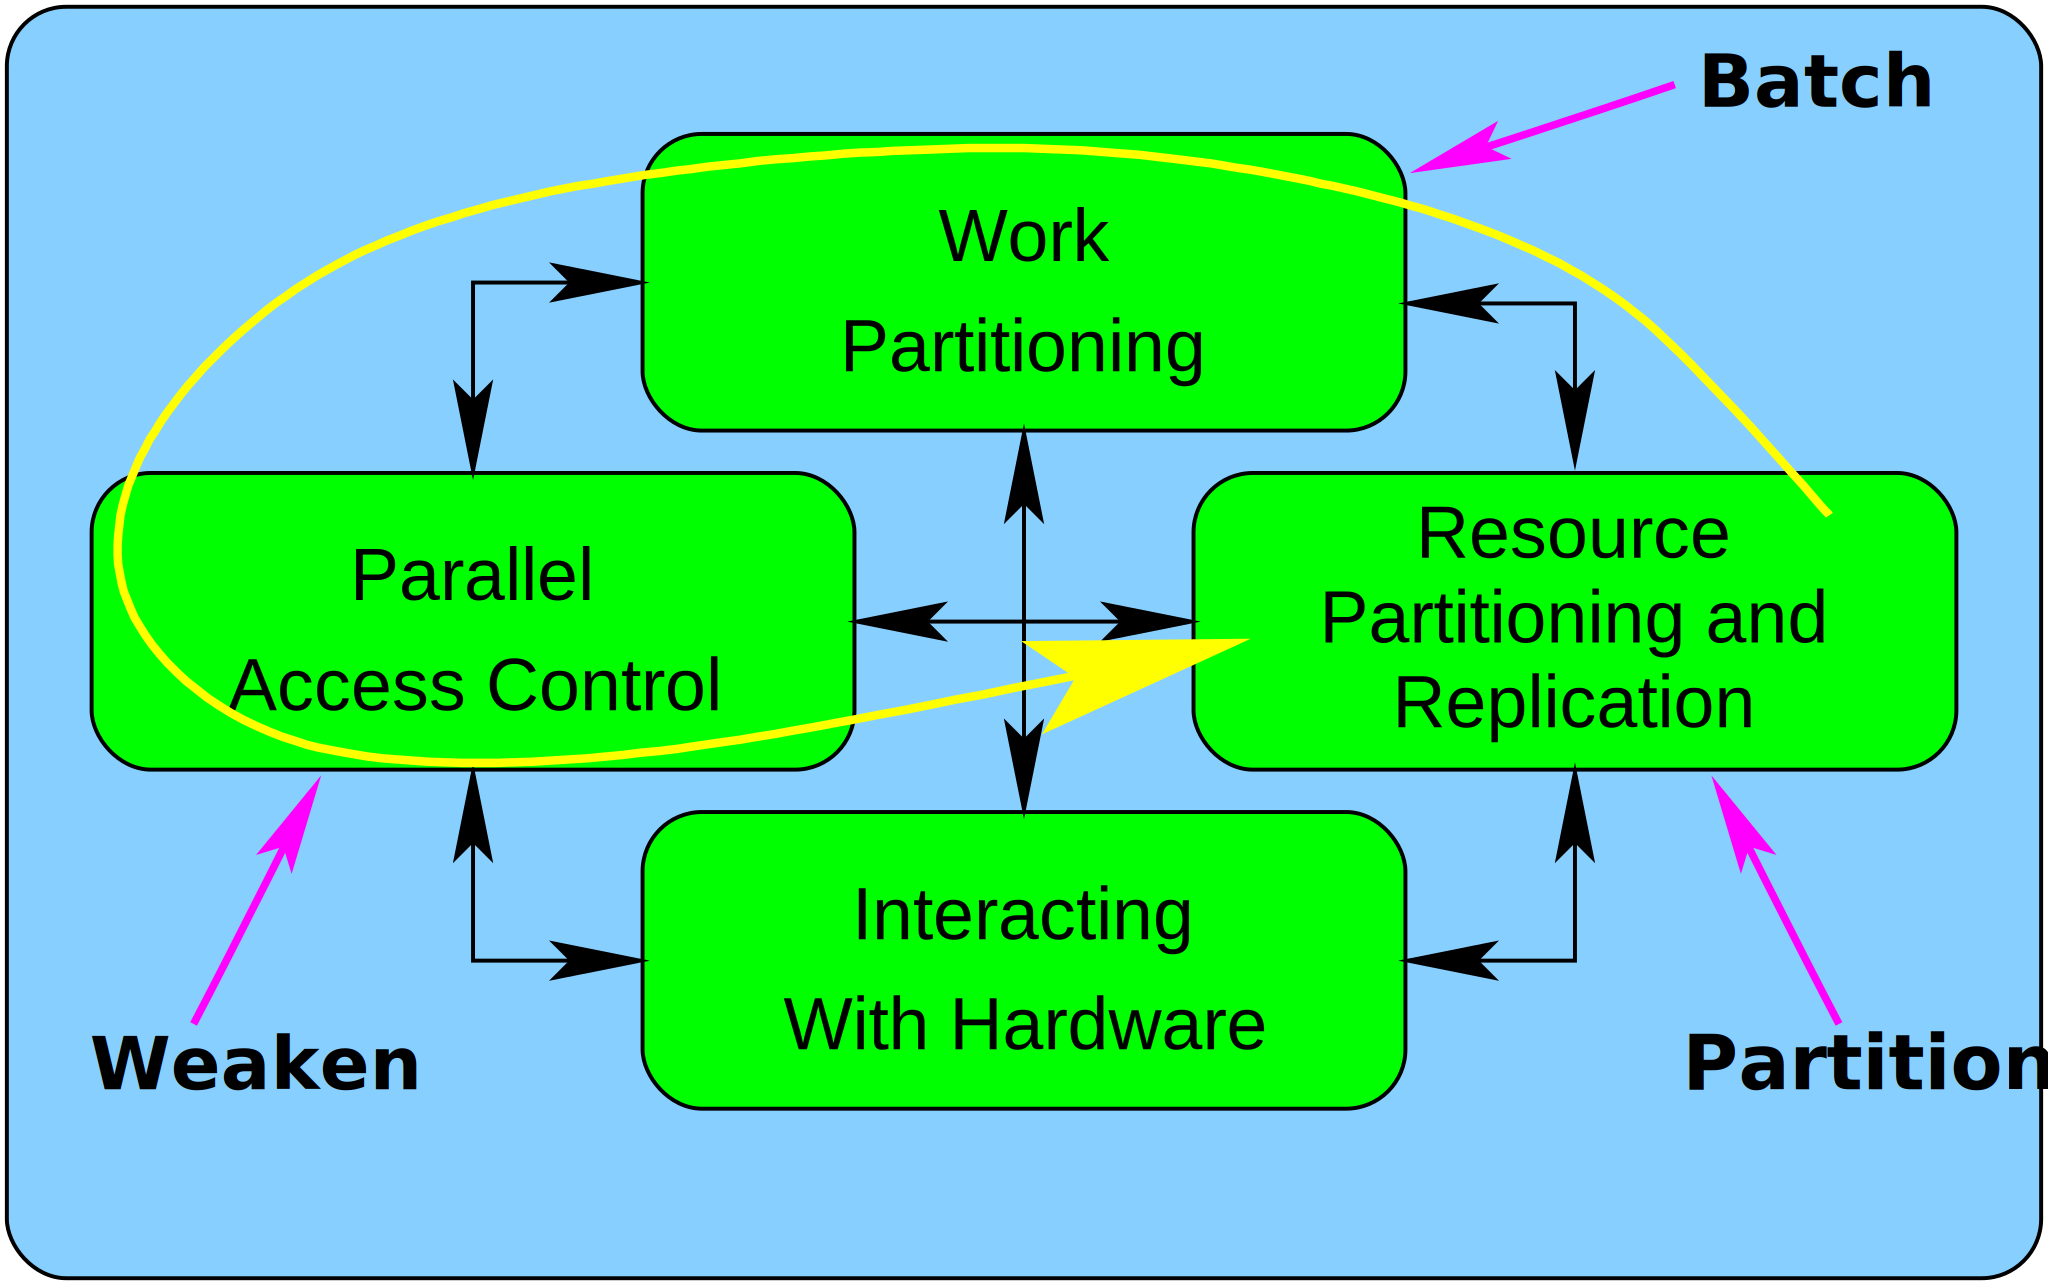
\includegraphics{count/FourTaskOrderOpt}}
\caption{Optimization and the Four Parallel-Programming Tasks}
\label{fig:count:Optimization and the Four Parallel-Programming Tasks}
\end{figure}

계속해서 요약해 보자면, 우린 성능과 확장성을 개선할 수 있는 ``세개의 커다란''
방법을 가지고 있는데, 각각
(1)~CPU 와 쓰레드들을 \emph{분할하기 (partitioning)},
(2)~한번의 비싼 동기화 오퍼레이션마다 더 많은 일이 처리되도록 \emph{몰아서
처리하기 (batching)}, 그리고
(3)~가능하다면 동기화 오퍼레이션들을 \emph{약화시키기}.
대략적 경험적 법칙상으로는,
page~\pageref{fig:intro:Ordering of Parallel-Programming Tasks} 의
Figure~\ref{fig:intro:Ordering of Parallel-Programming Tasks} 에서 이야기
한것처럼 이 방법들을 이 순서대로 적용해야 합니다.
분할하기 최적화 기법, 몰아서 처리하기 최적화 기법, 그리고 동기화 약화 최적화
기법은 각각
Figure~\ref{fig:count:Optimization and the Four Parallel-Programming Tasks}
의 ``리소스 분할하기와 복사하기'', ``일 분할하기'', ``병렬 접근 제어'' 에
적용될 수 있습니다.
물론, 당신이 digital signal processors (DSPs), field-programmable gate arrays
(FPGAs), 또는 general-purpose graphical processing units (GPGPUs) 와 같은
특별한 용도의 하드웨어를 사용한다면, 설계 과정에서 ``하드웨어와 상호작용하기''
부분에 큰 집중을 기울여야 할 겁니다.
예를 들어, GPGPU 의 하드웨어 쓰레드와 메모리 연결 구조는 조심스런 분할과
몰아처리하기 설계 결정에 큰 영향을 끼칠 겁니다.
\iffalse

Summarizing still further, we have the ``big three'' methods of
increasing performance and scalability, namely
(1)~\emph{partitioning} over CPUs or threads,
(2)~\emph{batching} so that more work can be done by each expensive
synchronization operations, and
(3)~\emph{weakening} synchronization operations where feasible.
As a rough rule of thumb, you should apply these methods in this order,
as was noted earlier in the discussion of
Figure~\ref{fig:intro:Ordering of Parallel-Programming Tasks}
on
page~\pageref{fig:intro:Ordering of Parallel-Programming Tasks}.
The partitioning optimization applies to the
``Resource Partitioning and Replication'' bubble,
the batching optimization to the ``Work Partitioning'' bubble,
and the weakening optimization to the ``Parallel Access Control'' bubble,
as shown in
Figure~\ref{fig:count:Optimization and the Four Parallel-Programming Tasks}.
Of course, if you are using special-purpose hardware such as
digital signal processors (DSPs), field-programmable gate arrays (FPGAs),
or general-purpose graphical processing units (GPGPUs), you may need
to pay close attention to the ``Interacting With Hardware'' bubble
throughout the design process.
For example, the structure of a GPGPU's hardware threads and memory
connectivity might richly reward very careful partitioning
and batching design decisions.
\fi

짧게 말해서, 이 챕터의 시작에서 이야기했듯, 카운팅의 단순성이 우리가 복잡한
동기화 도구들이나 정교한 구조체에 정신을 팔리지 않은채 기본적인 동시성 문제를
알아볼 수 있게 했습니다.
그런 동기화 도구들과 데이터 구조들은 뒤의 챕터들에서 다룹니다.
\iffalse

In short, as noted at the beginning of this chapter, the simplicity
of counting have allowed us to explore many
fundamental concurrency issues without the distraction of
complex synchronization primitives or elaborate data structures.
Such synchronization primitives and data structures are covered
in later chapters.
\fi
